\documentclass[oneside]{book} % Indica que el tipo de documento es un libro 
\usepackage[spanish]{babel} % Indica que usaremos caracteres propios del español
\usepackage[utf8]{inputenc} % Carga el juego de caracteres internacional UTF-8
\usepackage[document]{ragged2e} % Para usar el /justify y salto de linea con \\ y \n
\usepackage{amsthm} % ¿Para qué se usa?
\usepackage{amsmath} % Para alinear ecuaciones
\usepackage{amssymb} % ¿Para qué se usa?
\usepackage{amsbsy} % ¿Para qué se usa?
\usepackage{graphicx} % Para usar imagenes
\usepackage{hyperref} % Para que las referencias sean interactivas
\hypersetup{colorlinks,linkcolor={black},citecolor={white},urlcolor={red}}  
\usepackage{anysize} % Para modificar libremente el tamaño de hoja y margen
\usepackage{longtable} % Para ecuaciones alineadas
\usepackage{bm} % Para vectores unitarios
\usepackage{hyphenat} % Para corregir warnings
\usepackage{microtype} % Para evitar overfull \hbox
\usepackage{xcolor} % Para usar colores distintos de fuente
\usepackage[parfill]{parskip} % Para cambiar el estilo que se usa para distinguir entre párrafos contiguos

\setlength{\parindent}{0em} % Borramos la sangría por defecto
\setlength{\leftskip}{0pt} % Borramos la sangría por defecto

% -------NUEVOS ESTILOS PARA TEOREMAS Y DEFINICIONES-------

% Estilo para Teoremas y Definiciones
\newtheoremstyle{Teorema} % Nombre del estilo
{1cm} % Espacio por encima del Teorema
{1cm} % Espacio por debajo del Teorema
{\rm} % Fuente del cuerpo del Teorema
{0cm} % Indentado del titulo
{\bf} % Fuente de la cabecera del Teorema
{} % Puntuación que separa cabecera del cuerpo
{\newline} % Espacio entre cabecera y cuerpo
{\thmname{#1}\thmnumber{ #2}\textnormal{\thmnote{ (#3)}}} % Estilo del título

% Estilo para Observaciones
\newtheoremstyle{[Obs]} % Nombre del estilo
{0.5cm} % Espacio por encima del Teorema
{0cm} % Espacio por debajo del Teorema
{\rm} % Fuente del cuerpo del Teorema
{0cm} % Indentado del titulo
{\bf} % Fuente de la cabecera del Teorema
{\hfill\newline\newline} % Puntuación que separa cabecera del cuerpo
{0cm} % Espacio entre cabecera y cuerpo
{\thmname{#1}} % Estilo del título

% Estilo para Ejemplos
\newtheoremstyle{Ejemplos} % Nombre del estilo
{1cm} % Espacio por encima del Teorema
{1cm} % Espacio por debajo del Teorema
{\rm} % Fuente del cuerpo del Teorema
{0cm} % Indentado del titulo
{\bf} % Fuente de la cabecera del Teorema
{\hfill\newline\newline} % Puntuación que separa cabecera del cuerpo
{0cm} % Espacio entre cabecera y cuerpo
{\thmname{#1}\thmnumber{ #2}} % Estilo del título
 
% Definimos, con el estilo para Teoremas, los Ejercicios, Proposiciones, Corolario, Teorema, Definición, Nota, Notas y Lemma
\theoremstyle{Teorema}
\newtheorem{Definicion}{Definición}[chapter] 
\newtheorem{Notacion}[Definicion]{Notación}
\newtheorem{Teorema}[Definicion]{Teorema}
\newtheorem{Corolario}[Definicion]{Corolario}
\newtheorem{Ejercicio}[Definicion]{Ejercicio}
\newtheorem{Proposicion}[Definicion]{Proposición}
\newtheorem{Lema}[Definicion]{Lema}
\newtheorem{Nota}[Definicion]{Nota}
\newtheorem{Axioma}[Definicion]{Axioma}
\newtheorem{Pregunta}[Definicion]{Pregunta}

% Definimos, con el estilo para Ejemplos, los ejemplos
\theoremstyle{Ejemplos}
\newtheorem{Ejemplos}[Definicion]{Ejemplos}

% Definimos, con el estilo para Observaciones, las observaciones
\theoremstyle{[Obs]}
\newtheorem*{Obs}{[Observaciones]}

% Definimos el entorno de las demostraciones
\def\proof{\textbf{\underline{Demostración}}}
\def\endproof{}
\let\oldproof\proof
\renewcommand{\proof}{\setlength{\leftskip}{0.5cm}\color{gray}\oldproof}

% Definimos el entorno de las pruebas
\def\subproof{\textbf{\underline{Prueba}}}
\def\endproof{}
\let\oldsubproof\subproof
\renewcommand{\subproof}{\setlength{\leftskip}{1cm}\color{gray}\oldsubproof}

% Definimos el entorno de soluciones
\def\sol{\textbf{\underline{Solución}}}
\def\endsol{}

% ---------MACROS---------
\def \test {test}

% ---------COMANDOS PROPIOS---------
\newcommand{\card}[1]{\left|#1\right|} % Cardinalidad
\newcommand{\cerradura}[2][\test]{\ifx \test #1 {\overline{#2}} \else {cl_{#1}(#2)} \fi} % Cerradura
\newcommand{\frontera}[2][\test]{\ifx \test #1 {\partial(#2)} \else {\partial_{#1}(#2)} \fi} % Frontera
\newcommand{\borde}[2][\test]{\ifx \test #1 {b(#2)} \else {b_{#1}(#2)} \fi} % Borde
\newcommand{\abs}[1]{\left|#1\right|} % Valor absoluto
\newcommand{\absSymbol}{\left|\right.} % Simbolo de valor absoluto
\newcommand{\norm}[1]{\lVert#1\rVert} % Norma de un vector
\newcommand{\normSymbol}{\lVert} % Simbolo de norma
\renewcommand{\{}{\left\lbrace} % Llave izquierda
\renewcommand{\}}{\right\rbrace} % Llave derecha
\renewcommand{\o}{\ \vee \ } % Simbolo del o lógico
\newcommand{\y}{\ \wedge\ } % Simbolo del y lógico
\renewcommand{\u}{\cup} % Simbolo de unión
\newcommand{\n}{\cap} % Simbolo de intersección
\newcommand{\U}{\bigcup} % Simbolo de unión desde i hasta n
\newcommand{\N}{\bigcap} % Simbolo de intersección desde i hasta n
\newcommand{\darkmode}{\usepackage{xcolor}\pagecolor{black\color{white}}} % Activa o desactiva el modo oscuro
\renewcommand{\sc}{\subseteq} % Simbolo de subconjunto
\newcommand{\Sc}{\supseteq} % Simbolo de superconjunto
\newcommand{\scp}{\subsetneq} % Simbolo de subconjunto propio
\newcommand{\nv}{\neq \emptyset} % Simbolo de es no vacio
\newcommand{\R}{\mathbb{R}} % Simbolo de R
\newcommand{\Z}{\mathbb{Z}} % Simbolo de Z
\newcommand{\Q}{\mathbb{Q}} % Simbolo de Q
\newcommand{\I}{\mathbb{I}} % Simbolo de I
\newcommand{\C}{\mathbb{C}} % Simbolo de C
\newcommand{\Rn}{\mathbb{R}^n} % Simbolo de R^n
\renewcommand{\P}{\mathcal{P}} % Simbolo de potencia
\newcommand{\Ri}[1]{\mathbb{R}^{#1}} % Simbolo de R^n variable
\renewcommand{\qed}{$\blacksquare$} % Simbolo de Q.E.D
\newcommand{\subqed}{$\square$} % Simbolo de Q.E.D blanco
\newcommand{\NuevoInciso}{\vspace{2cm}} % Espaciado entre Incisos
\newcommand{\pd}{$\vdash\ $} % Simbolo de por demostrar
\renewcommand{\c}{$!!!\ $} % Simbolo de contradicción
\newcommand{\necesidad}{$\Rightarrow]\ $} % Simbolo para indicar que se prueba la necesidad
\newcommand{\suficiencia}{$\Leftarrow]\ $} % Simbolo para indicar que se prueba la suficiencia
\newcommand{\Imp}{$\Rightarrow\ $} % Implicación sin justificación
\newcommand{\nsc}{\nsubseteq} % Negación del símbolo de subconjunto
\newcommand{\grad}{\triangledown} % Simbolo de gradiente
\newcommand{\parcialC}[2]{\frac{\partial #1}{\partial #2}} % Parcial de una función respecto a una variable
\newcommand{\parcialL}[2]{\frac{\partial}{\partial #2} \left( #1 \right)} % Parcial de una función (larga) respecto a una variable
\newcommand{\comment}[1]{} % Para comandos multilinea
\newcommand{\indentar}[2]{{\setlength{\leftskip}{#1} #2 \setlength{\leftskip}{0cm}}} % Subcasos

% Vectores i, j y k
\newcommand{\vi}{{\bm{\hat{\textnormal{\bfseries\i}}}}}
\newcommand{\vj}{{\bm{\hat{\textnormal{\bfseries\j}}}}}
\newcommand{\vk}{{\bm{\hat{\textnormal{\bfseries k}}}}}

% Para integrales
\newcommand{\sdint}[3]{\lefteqn{\displaystyle\iint \limits_{#1}^{} #2}\lefteqn{\hspace{1.2ex}\rule[3.35ex]{2.7ex}{0.15ex}}
\phantom{\displaystyle\iint \limits_{#1}^{} #2} \ #3}
\newcommand{\idint}[3]{\lefteqn{\displaystyle\iint \limits_{#1}^{} #2}\lefteqn{\hspace{0.0ex}\rule[-2.25ex]{2.7ex}{0.15ex}}
\phantom{\displaystyle\iint \limits_{#1}^{} #2} \ #3}
\newcommand{\dint}[3]{\displaystyle\iint \limits_{#1}^{} #2 \ #3}
\newcommand{\stint}[3]{\lefteqn{\displaystyle\iiint \limits_{#1}^{} #2}\lefteqn{\hspace{1.2ex}\rule[3.35ex]{4.1ex}{0.15ex}}
\phantom{\displaystyle\iiint \limits_{#1}^{} #2} \ #3}
\newcommand{\itint}[3]{\lefteqn{\displaystyle\iiint \limits_{#1}^{} #2}\lefteqn{\hspace{0.0ex}\rule[-2.25ex]{4.1ex}{0.15ex}}
\phantom{\displaystyle\iiint \limits_{#1}^{} #2} \ #3}
\newcommand{\tint}[3]{\displaystyle\iiint \limits_{#1}^{} #2 \ #3}
\newcommand{\snint}[3]{\lefteqn{\displaystyle\idotsint \limits_{#1}^{} #2}\lefteqn{\hspace{1.2ex}\rule[3.35ex]{6.8ex}{0.15ex}}
\phantom{\displaystyle\idotsint \limits_{#1}^{} #2} \ #3}
\newcommand{\inint}[3]{\lefteqn{\displaystyle\idotsint \limits_{#1}^{} #2}\lefteqn{\hspace{0.0ex}\rule[-2.25ex]{6.8ex}{0.15ex}}
\phantom{\displaystyle\idotsint \limits_{#1}^{} #2} \ #3}
\newcommand{\nint}[3]{\displaystyle\idotsint \limits_{#1}^{} #2 \ #3}
\newcommand{\lints}[2]{\int \limits_{#1}^{#2}}
\newcommand{\lint}[4]{\int \limits_{#1}^{#2} #3 \ d#4}
\newcommand{\dlint}[3]{\int \limits_{#1}^{#2} #3}

% Para integrales cerradas
\newcommand{\olints}[2]{\oint \limits_{#1}^{#2}}
\newcommand{\olint}[4]{\oint \limits_{#1}^{#2} #3 \ d#4}
\newcommand{\odlint}[3]{\oint \limits_{#1}^{#2} #3}

% Para limites
\newcommand{\limite}[2]{\displaystyle\lim_{#1} #2}

\pagenumbering{gobble} % Evitar errores
\makeindex

\begin{document}

    % Para evitar errores de compilación
	\color{white} 
	Cita de ejemplo: \cite{DUMMY:1}
	\color{black} \newpage
	\pagenumbering{arabic}

	\begin{titlepage}
		\centering
		{\bfseries\LARGE Benmérita Universidad Autónoma de Puebla \par}
		\vspace{1cm}
		{\scshape\Large Facultad de Ciencias Físico Matemáticas \par}
		\vspace{3cm}
		{\scshape\Huge Análisis Matemático en Espacios Métricos \par}
		\vspace{3cm}
		{\itshape\Large Notas de clase \par}
		\vfill
		{\Large Luis Alfredo Monroy Villegas \par}
		{\Large Servicio Social \par}
		\vfill
		{\Large Otoño 2023 \par}
	\end{titlepage}

	\tableofcontents
	\justify
	\title{Análisis Matemático en Espacios Métricos}

	\chapter{Espacios Métricos}

		\section{Definición, equivalencias y propiedades básicas}

			\begin{Definicion}[Espacio Pseudométrico]\setlength{\parindent}{0em}
				
				Una dupla $(M, d)$ donde $M$ es un conjunto no vacio y $d$ es una función $d : M \times M \to \R$ es un espacio pseudométrico si satisface que para cualesquiera $x, y, z \in M$ se cumplen: 

				\textbf{1)} $d(x, x) = 0$ 

				\textbf{2)} $d(x, y) \geq 0$ 

				\textbf{3)} $d(x, y) = d(y, x)$ 

				\textbf{4)} $d(x, y) \leq d(x, z) + d(y, z)$ 

				\begin{Obs}
				
					\textbf{1.} A los elementos de $M$ les llamaremos puntos

					\textbf{2.} A $d$ se le llama pseudométrica (O écart) de $M$ o del espacio $(M, d)$

					\textbf{3.} A \textbf{$4)$} se le conoce como desigualdad del triángulo

					\textbf{4.} A \textbf{$3)$} se le conoce como simetría (De la pseudométrica)
				
				\end{Obs}

			\end{Definicion}

			\begin{Definicion}[Espacio Métrico]\setlength{\parindent}{0em}

				Una dupla $(M, d)$ donde $M$ es un conjunto no vacio y $d$ es una función $d : M \times M \to \R$ es un espacio métrico si satisface que para cualesquiera $x, y, z \in M$ se cumplen: 

				\textbf{1)} $d(x, x) = 0$ 

				\textbf{2)} $x \neq y$ \Imp $d(x, y) > 0$ 

				\textbf{3)} $d(x, y) = d(y, x)$ 

				\textbf{4)} $d(x, y) \leq d(x, z) + d(y, z)$ 

				\begin{Obs}

					\textbf{1.} A los elementos de $M$ les llamaremos puntos

					\textbf{2.} A $d$ se le llama métrica de $M$ o del espacio $(M, d)$ 

					\textbf{3.} A \textbf{$4)$} se le conoce como desigualdad del triángulo

					\textbf{4.} A \textbf{$3)$} se le conoce como simetría (De la métrica)
				
				\end{Obs}

			\end{Definicion}

			\begin{Proposicion}\setlength{\parindent}{0em}

				Sean $M$ un conjunto no vacio y $d$ una función $d : M \times M \to \R$. $(M, d)$ es un espacio pseudométrico si y sólo si para cualesquiera $x, y, z \in M$ se cumplen: 

				\textbf{1)} $d(x, x) = 0$ 

				\textbf{2)} $d(x, y) \geq 0$
				
				\textbf{3)} $d(x, y) = d(y, x)$ 

				\textbf{4)} $d(x, y) \leq d(x, z) + d(z, y)$

				\begin{proof}
					
					Sean $M$ un conjunto no vacio, $d$ una función $d : M \times M \to \R$ y $x, y, z \in M$ \\
					\pd $(M, d)$ es un espacio pseudométrico $\Leftrightarrow$ $d$ satisface \textbf{1) - 4)}

					\necesidad Sup. $(M, d)$ es un espacio pseudométrico \\
					\pd $d$ satisface \textbf{1) - 4)}

					Directamente de la definición $d$ satisface \textbf{1)}, \textbf{2)} y \textbf{3)} por lo que resta ver que $d(x, y) \leq d(x, z) + d(z, y)$
					
					Aplicando la desigualdad del triangulo tenemos que $d(x, y) \leq d(x, z) + d(y, z)$ pero aplicando la simetría tenemos que $d(y, z) = d(z, y)$ por tanto $d(x, y) \leq d(x, z) + d(z, y)$

					\suficiencia Sup. $d$ satisface \textbf{1) - 4)} \\
					\pd $(M, d)$ es un espacio pseudométrico

					Por Definición de espacio pseudométrico bastará con probar que $d$ satisface la desigualdad del triángulo
					
					Por la propiedad \textbf{4)}, $d(x, y) \leq d(x, z) + d(z, y)$ pero por la propiedad \textbf{3)} $d(z, y) = d(y, z)$ asi que $d(x, y) \leq d(x, z) + d(y, z)$ por lo que $d$ cumple la desigualdad triangular \qed

				\end{proof}

			\end{Proposicion}

			\begin{Proposicion}\setlength{\parindent}{0em}

				Sean $M$ un conjunto no vacio y $d$ una función $d : M \times M \to \R$. $(M, d)$ es un espacio métrico si y sólo si para cualesquiera $x, y, z \in M$ se cumplen: 

				\textbf{1)} $d(x, x) = 0$ 

				\textbf{2)} $x \neq y \Rightarrow d(x, y) > 0$
				
				\textbf{3)} $d(x, y) = d(y, x)$ 

				\textbf{4)} $d(x, y) \leq d(x, z) + d(z, y)$

				\begin{proof}
					
					Sean $M$ un conjunto no vacio, $d$ una función $d : M \times M \to \R$ y $x, y, z \in M$ \\
					\pd $(M, d)$ es un espacio métrico $\Leftrightarrow$ $d$ satisface \textbf{1) - 4)}

					\necesidad Sup. $(M, d)$ es un espacio métrico \\
					\pd $d$ satisface \textbf{1) - 4)}

					Directamente de la definición $d$ satisface \textbf{1)}, \textbf{2)} y \textbf{3)} por lo que resta ver que $d(x, y) \leq d(x, z) + d(z, y)$
					
					Aplicando la desigualdad del triangulo tenemos que $d(x, y) \leq d(x, z) + d(y, z)$ pero aplicando la simetría tenemos que $d(y, z) = d(z, y)$ por tanto $d(x, y) \leq d(x, z) + d(z, y)$

					\suficiencia Sup. $d$ satisface \textbf{1) - 4)} \\
					\pd $(M, d)$ es un espacio métrico

					Por Definición de espacio métrico bastará con probar que $d$ satisface la desigualdad del triángulo
					
					Por la propiedad \textbf{4)}, $d(x, y) \leq d(x, z) + d(z, y)$ pero por la propiedad \textbf{3)} $d(z, y) = d(y, z)$ asi que $d(x, y) \leq d(x, z) + d(y, z)$ por lo que $d$ cumple la desigualdad triangular \qed

				\end{proof}

			\end{Proposicion}

			\begin{Lema}\label{Lema: Primer lema de metricas}\setlength{\parindent}{0em}
				
				Sea $(M, d)$ un espacio pseudométrico, entonces 

				\[ \forall x, y, z, t \in M : \abs{d(x, y) - d(z, t)} \leq d(x, z) + d(y, t) \] 

				\begin{proof}
					
					Sean $(M, d)$ un espacio pseudométrico y $x, y, z \in M$ \\
					\pd $\abs{d(x, y) - d(z, t)} \leq d(x, z) + d(y, t)$

					Aplicando la desiguladad triangular dos veces, tenemos que 
					
					\[ d(x, y) \leq d(x, z) + d(y, z) \leq d(x, z) + d(y, t) + d(z, t) \] 
					
					En consecuencia
					
					\[ d(x, y) \leq d(x, z) + d(y, t) + d(z, t) \] 
					
					Por lo que
					
					\begin{equation*}\tag{$\star$}
						d(x, y) - d(z, t) \leq d(x, z) + d(y, t)
					\end{equation*}

					Por otro lado aplicando la propiedad simétrica y la desigualdad triangular dos veces llegamos a que
					
					\begin{align*}
						d(z, t) & \leq d(z, x) + d(t, x) \\
						& \leq d(z, x) + d(t, y) + d(x, y) \\
						& = d(x, y) + d(z, x) + d(t, y) \\  
						& = d(x, y) + d(x, z) + d(y, t)
					\end{align*}
					
					Por lo que 
					
					\[ d(z, t) \leq d(x, y) + d(x, z) + d(y, t) \]
					
					En consecuencia 

					\begin{equation*}\tag{$\star\star$}
						- (d(x, z) + d(y, t)) \leq d(x, y) - d(z, t)
					\end{equation*}

					Juntando las desigualdades $\star$ y $\star\star$ tenemos que 

					\begin{equation*}
						- (d(x, z) + d(y, t)) \leq d(x, y) - d(z, t) \leq d(x, z) + d(y, t)
					\end{equation*}

					Por tanto $\abs{d(x, y) - d(z, t)} \leq d(x, z) + d(y, t)$ \qed

				\end{proof}

			\end{Lema}

			\begin{Corolario}\setlength{\parindent}{0em}

				Sea $(M, d)$ un espacio pseudométrico, entonces 

				\[ \forall x, y, z \in M : \abs{d(x, z) - d(y, z)} \leq d(x, y) \] 

				\begin{proof}
					
					Sean $(M, d)$ un espacio pseudométrico y $x, y, z \in M$ \\
					\pd $\abs{d(x, z) - d(y, z)} \leq d(x, y)$

					Por el Lema anterior tenemos que $\abs{d(x, z) - d(y, z)} \leq d(x, y) + d(z, z) = d(x, y) + 0 = d(x, y)$ por tanto $\abs{d(x, z) - d(y, z)} \leq d(x, y)$ \qed

				\end{proof}

			\end{Corolario}

			\noindent La siguiente proposición nos permitirá extender estas propiedades a Espacios Métricos.

			\begin{Proposicion}\setlength{\parindent}{0em}
				
				Sea $(M, d)$ un espacio métrico, entonces $(M, d)$ es un espacio pseudométrico.

				\begin{proof}
					
					Sean $(M, d)$ un espacio métrico \\
					\pd $(M, d)$ es un espacio pseudométrico

					Por definición para cualesquiera $x, y, z \in M$ se cumple que $d(x, x) = 0$, $d(x, y) = d(y, x)$ y que $d(x, y) \leq d(x, z) + d(y, z)$ por lo que resta ver que $d(x, y) \geq 0$. Si $x = y$, entonces $d(x, y) = d(x, x) = 0$ y si $x \neq y$, entonces $d(x, y) > 0$ por ser $(M, d)$ espacio métrico por tanto $d(x, y) \geq 0$ y en consecuencia $(M, d)$ es un espacio pseudométrico \qed 

				\end{proof}

			\end{Proposicion}

			\begin{Proposicion}\setlength{\parindent}{0em}

				Sean $M$ un conjunto no vacio y $d$ una función $d : M \times M \to \R$. $(M, d)$ es un espacio métrico si y sólo si para cualesquiera $x, y, z \in M$ se cumplen: 

				\textbf{1)} $d(x, y) \geq 0$ 

				\textbf{2)} $d(x, y) = 0 \Leftrightarrow x = y$ 

				\textbf{3)} $d(x, y) \leq d(x, z) + d(y, z)$
				
				\begin{proof}
					
					Sean $M$ un conjunto no vacio, $d$ una función $d : M \times M \to \R$ y $x, y, z \in M$ \\
					\pd $(M, d)$ es un espacio métrico $\Leftrightarrow$ $d$ satisface \textbf{1) - 3)}

					\necesidad Sup. $(M, d)$ es un espacio métrico \\
					\pd $d$ satisface \textbf{1) - 3)}

					Directamente de la definición de espacio métrico, tenemos que $d$ satisface \textbf{3)}, por otro lado $(M, d)$ es en particular un espacio pseudométrico por lo que tambien satisface \textbf{1)}.
					
					Finalmente para \textbf{2)}, si $x = y$ entonces $d(x, y) = d(x, x) = 0$ asi que $x = y$ \Imp $d(x, y) = 0$ y sabemos que $x \neq y$ \Imp $d(x, y) > 0$ asi que por contrapositiva (Y del hecho que $d(x, y) \geq 0$), $d(x, y) = 0$ \Imp $x = y$ por tanto $x = y \Leftrightarrow d(x, y) = 0$ y en consecuencia $d$ satisface \textbf{1) - 3)}.

					\suficiencia Sup. $d$ satisface \textbf{1) - 3)} \\
					\pd $(M, d)$ es un espacio métrico

					\textbf{a)} \pd $d(x, x) = 0$ \\
					Por la propiedad \textbf{2)} como $x = x$ tenemos que $d(x, x) = 0$

					\textbf{b)} Sup. $x \neq y$ \\
					\pd $d(x, y) > 0$ \\
					Supongamos que es falso que $d(x, y) > 0$, por la propiedad \textbf{1)} debe ocurrir que $d(x, y) = 0$ y por la propiedad \textbf{2)} tambien $x = y$ \c por tanto $d(x, y) > 0$

					\textbf{c)} \pd $d(x, y) = d(y, x)$ \\
					Aplicando la propiedad \textbf{3)} tenemos que $d(x, y) \leq d(x, x) + d(y, x) = 0 + d(y, x) = d(y, x)$ por lo que $d(x, y) \leq d(y, x)$ pero tambien $d(y, x) \leq d(y, y) + d(x, y) = 0 + d(x, y) = d(x, y)$ asi que $d(y, x) \leq d(x, y)$ luego $d(x, y) = d(y, x)$ 

					\textbf{d)} \pd $d(x, y) \leq d(x, z) + d(y, z)$ \\
					Se tiene por hipótesis usando la propiedad \textbf{3)}

					Por \textbf{a) - d)} podemos concluir que $(M, d)$ es un espacio métrico \qed

				\end{proof}

			\end{Proposicion}

			\begin{Proposicion}\setlength{\parindent}{0em}

				Sean $M$ un conjunto no vacio y $d$ una función $d : M \times M \to \R$. $(M, d)$ es un espacio métrico si y sólo si para cualesquiera $x, y, z \in M$ se cumplen: 

				\textbf{1)} $d(x, y) = 0 \Leftrightarrow x = y$ 

				\textbf{2)} $d(x, y) \leq d(x, z) + d(y, z)$ 

				\begin{proof}
					
					Sean $M$ un conjunto no vacio, $d$ una función $d : M \times M \to \R$ y $x, y, z \in M$ \\
					\pd $(M, d)$ es un espacio métrico $\Leftrightarrow$ $d$ satisface \textbf{1)} y \textbf{2)}

					\necesidad Sup. $(M, d)$ es un espacio métrico \\
					\pd $d$ satisface \textbf{1)} y \textbf{2)}

					Por la Proposición anterior se cumplen \textbf{1)} y \textbf{2)} directamente 

					\suficiencia Sup. $d$ satisface \textbf{1)} y \textbf{2)} \\
					\pd $(M, d)$ es un espacio métrico

					Por la Proposición anterior, bastará probar que $d(x, y) \geq 0$. Por la propiedad \textbf{2)} tenemos que $0 = d(x, x) \leq d(x, y) + d(x, y) = 2d(x, y)$ por lo que $2d(x, y) \geq 0$ luego $d(x, y) \geq 0$ \qed

				\end{proof}

			\end{Proposicion}

			\begin{Ejemplos}\label{Ejemplos: Metricas basicas}\setlength{\parindent}{0em}

				\textbf{1.} $(\R, d)$ donde $d(x, y) = \abs{x - y}$ para cualesquiera $x, y \in \R$ es un espacio métrico. 
				
				\begin{proof}
					
					Sean $x, y, z \in \R$ y $d(x, y) := \abs{x - y}$

					\textbf{a)} \pd $d(x, x) = 0$ \\
					Se tiene que $d(x, x) = \abs{x - x} = \abs{0} = 0$ por tanto $d(x, x) = 0$ 

					\textbf{b)} Sup. $x \neq y$ \\
					\pd $d(x, y) > 0$ \\
					Como $d(x, y) = \abs{x - y} > 0$, entonces $d(x, y) > 0$ 

					\textbf{c)} \pd $d(x, y) = d(y, x)$ \\
					Se tiene que $d(x, y) = \abs{x - y} = \abs{y - x} = d(y, x)$ luego $d(x, y) = d(y, x)$ 

					\textbf{d)} \pd $d(x, y) \leq d(x, z) + d(z, y)$ \\
					Por la desigualdad del triangulo tenemos que $d(x, y) = \abs{x - y} = \abs{(x - z) + (z - y)} \leq \abs{x - z} + \abs{z - y} = d(x, z) + d(z, y)$ por tanto $d(x, y) \leq d(x, z) + d(z, y)$ 

					Por \textbf{a) - d)}, tenemos que $(\R, d)$ es un espacio métrico \qed 

				\end{proof}
				
				\textbf{2.} $(\C, d)$ donde $d(z_1, z_2) = \abs{z_1 - z_2}$ para cualesquiera $z_1, z_2 \in \C$ es un espacio métrico. 

				\begin{proof}
					
					Sean $z_1, z_2, z_3 \in \C$ y $d(z_1, z_2) := \abs{z_1 - z_2}$

					\textbf{a)} \pd $d(z_1, z_1) = 0$ \\
					Se tiene que $d(z_1, z_1) = \abs{z_1 - z_1} = \abs{0} = 0$ por tanto $d(z_1, z_1) = 0$ 

					\textbf{b)} Sup. $z_1 \neq z_2$ \\
					\pd $d(z_1, z_2) > 0$ \\
					Como $d(z_1, z_2) = \abs{z_1 - z_2} > 0$, entonces $d(z_1, z_2) > 0$ 

					\textbf{c)} \pd $d(z_1, z_2) = d(z_2, z_1)$ \\
					Se tiene que $d(z_1, z_2) = \abs{z_1 - z_2} = \abs{z_2 - z_1} = d(z_2, z_1)$ luego $d(z_1, z_2) = d(z_2, z_1)$ 

					\textbf{d)} \pd $d(z_1, z_2) \leq d(z_1, z_3) + d(z_3, z_2)$ \\
					Tenemos que $d(z_1, z_2) = \abs{z_1 - z_2} = \abs{(z_1 - z_3) + (z_3 - z_2)} \leq \abs{z_1 - z_3} + \abs{z_3 - z_2} = d(z_1, z_3) + d(z_3, z_2)$ por tanto $d(z_1, z_2) \leq d(z_1, z_3) + d(z_3, z_2)$ 

					Por \textbf{a) - d)}, tenemos que $(\C, d)$ es un espacio métrico \qed 

				\end{proof}
				
				\textbf{3.} $(\Rn, d)$ donde $d(x, y) = \norm{x - y}$ para cualesquiera $x, y \in \Rn$ es un espacio métrico llamado espacio Euclidiano. 

				\begin{proof}
					
					Sean $x, y, z \in \Rn$ y $d(x, y) := \norm{x - y}$

					\textbf{a)} \pd $d(x, x) = 0$ \\
					Se tiene que $d(x, x) = \norm{x - x} = \norm{0} = 0$ por tanto $d(x, x) = 0$ 

					\textbf{b)} Sup. $x \neq y$ \\
					\pd $d(x, y) > 0$ \\
					Como $d(x, y) = \norm{x - y} > 0$, entonces $d(x, y) > 0$ 

					\textbf{c)} \pd $d(x, y) = d(y, x)$ \\
					Se tiene que $d(x, y) = \norm{x - y} = \norm{y - x} = d(y, x)$ luego $d(x, y) = d(y, x)$ 

					\textbf{d)} \pd $d(x, y) \leq d(x, z) + d(z, y)$ \\
					Por la desigualdad del triangulo tenemos que $d(x, y) = \norm{x - y} = \norm{(x - z) + (z - y)} \leq \norm{x - z} + \norm{z - y} = d(x, z) + d(z, y)$ por tanto $d(x, y) \leq d(x, z) + d(z, y)$ 

					Por \textbf{a) - d)}, tenemos que $(\Rn, d)$ es un espacio métrico \qed 

				\end{proof}
				
				\textbf{4.} $(\Rn, d)$ donde para cualesquiera $(x_1, x_2, ..., x_n), (y_1, y_2, ..., y_n) \in \Rn$, $d( (x_1, x_2, ..., x_n), (y_1, y_2, ..., y_n) ) = \abs{x_1 - y_1} + \abs{x_2 - y_2} + ... + \abs{x_n - y_n}$ es un espacio métrico. 

				\begin{proof}
					
					Sean $x, y, z \in \R$ tales que $x = (x_1, x_2, ..., x_n), y = (y_1, y_2, ..., y_n), z = (z_1, z_2, ..., z_n)$ y $d(x, y) := \abs{x_1 - y_1} + \abs{x_2 - y_2} + ... + \abs{x_n - y_n}$

					\textbf{a)} \pd $d(x, x) = 0$ \\
					Se tiene que $d(x, x) = \abs{x_1 - x_1} + \abs{x_2 - x_2} + ... + \abs{x_n - x_n} = 0 + 0 + ... + 0 = 0$ por tanto $d(x, x) = 0$ 

					\textbf{b)} Sup. $x \neq y$ \\
					\pd $d(x, y) > 0$ \\
					Como $x \neq y$ existe un $i \in \{ 1, 2, ..., n \}$ tal que $x_i \neq y_i$ luego $\abs{x_i - y_i} > 0$ por lo que por tener un sumando mayor a cero, tambien $\abs{x_1 - y_1} + \abs{x_2 - y_2} + ... + \abs{x_n - y_n} > 0$, es decir $d(x, y) > 0$ 

					\textbf{c)} \pd $d(x, y) = d(y, x)$ \\
					Se tiene que $d(x, y) = \abs{x_1 - y_1} + \abs{x_2 - y_2} + ... + \abs{x_n - y_n} = \abs{y_1 - x_1} + \abs{y_2 - x_2} + ... + \abs{y_n - x_n} = d(y, x)$ luego $d(x, y) = d(y, x)$ 

					\textbf{d)} \pd $d(x, y) \leq d(x, z) + d(z, y)$ \\
					Por la desigualdad del triangulo tenemos que para cada $i \in \{ 1, 2, ..., n \}$, se cumple que $\abs{x_i - y_i} = \abs{(x_i - z_i) + (z_i - y_i)} \leq \abs{x_i - z_i} + \abs{z_i - y_i}$ por lo que $d(x, y) = \abs{x_1 - y_1} + \abs{x_2 - y_2} + ... + \abs{x_n - y_n} \leq (\abs{x_1 - z_1} + \abs{z_1 - y_1}) + (\abs{x_2 - z_2} + \abs{z_2 - y_2}) + ... + (\abs{x_n - z_n} + \abs{z_n - y_n}) = (\abs{x_1 - z_1} + \abs{x_2 - z_2} + ... + \abs{x_n - z_n}) + (\abs{z_1 - y_1} + \abs{z_2 - y_2} + ... + \abs{z_n - y_n}) = d(x, z) + d(z, y)$ por tanto $d(x, y) \leq d(x, z) + d(z, y)$

					Por \textbf{a) - d)}, tenemos que $(\Rn, d)$ es un espacio métrico \qed 

				\end{proof}
				
				\textbf{5.} $(\Rn, d)$ donde para cualesquiera $(x_1, x_2, ..., x_n), (y_1, y_2, ..., y_n) \in \Rn$, $d( (x_1, x_2, ..., x_n), (y_1, y_2, ..., y_n) ) = \max\{ \abs{x_1 - y_1}, \abs{x_2 - y_2}, ..., \abs{x_n - y_n} \}$ es un espacio métrico. 

				\begin{proof}
					
					Sean $x, y, z \in \R$ tales que $x = (x_1, x_2, ..., x_n), y = (y_1, y_2, ..., y_n), z = (z_1, z_2, ..., z_n)$ y $d(x, y) := \max\{\abs{x_1 - y_1}, \abs{x_2 - y_2}, ..., \abs{x_n - y_n}\}$

					\textbf{a)} \pd $d(x, x) = 0$ \\
					Se tiene que $d(x, x) = \max\{\abs{x_1 - x_1}, \abs{x_2 - x_2}, ..., \abs{x_n - x_n}\} = \max\{ 0, 0, ..., 0 \} = \max\{ 0 \} = 0$ por tanto $d(x, x) = 0$ 

					\textbf{b)} Sup. $x \neq y$ \\
					\pd $d(x, y) > 0$ \\
					Como $x \neq y$ existe un $i \in \{ 1, 2, ..., n \}$ tal que $x_i \neq y_i$ luego $\abs{x_i - y_i} > 0$ por lo que por ser cota superior de $\{\abs{x_1 - y_1}, \abs{x_2 - y_2}, ..., \abs{x_n - y_n}\}$ tenemos que $\max\{\abs{x_1 - y_1}, \abs{x_2 - y_2}, ..., \abs{x_n - y_n}\} \geq \abs{x_i - y_i} > 0$, es decir $d(x, y) > \abs{x_i - y_i} > 0$ luego $d(x, y) > 0$ 

					\textbf{c)} \pd $d(x, y) = d(y, x)$ \\
					Se tiene que $d(x, y) = \max\{\abs{x_1 - y_1}, \abs{x_2 - y_2}, ..., \abs{x_n - y_n}\} = \max\{\abs{y_1 - x_1}, \abs{y_2 - x_2}, ..., \abs{y_n - x_n}\} = d(y, x)$ luego $d(x, y) = d(y, x)$ 

					\textbf{d)} \pd $d(x, y) \leq d(x, z) + d(z, y)$ \\
					Por la desigualdad del triangulo tenemos que para cada $i \in \{ 1, 2, ..., n \}$, se cumple que $\abs{x_i - y_i} = \abs{(x_i - z_i) + (z_i - y_i)} \leq \abs{x_i - z_i} + \abs{z_i - y_i}$ asi que: 
					
					$d(x, y)$
					$=\max\{ \abs{x_1 - y_1}, \abs{x_2 - y_2}, ...,\abs{x_n - y_n} \}$ \\
					$\leq \max\{ \abs{x_1 - z_1} + \abs{z_1 - y_1}, \abs{x_2 - z_2} + \abs{z_2 - y_2}, ...,\abs{x_n - z_n} + \abs{z_n - y_n} \}$ \\
					$\leq \max\{ \abs{x_1 - z_1}, \abs{x_2 - z_2}, ...,\abs{x_n - z_n} \} + \max\{ \abs{z_1 - y_1}, \abs{z_2 - y_2}, ..., \abs{z_n - y_n} \}$ \\
					$= d(x, z) + d(z, y)$
					
					Por tanto $d(x, y) \leq d(x, z) + d(z, y)$

					Por \textbf{a) - d)}, tenemos que $(\Rn, d)$ es un espacio métrico \qed 

				\end{proof}

				\textbf{6.} $(\Ri{2}, d)$ donde para cualesquiera $(x_1, x_2), (y_1, y_2) \in \Ri{2}$, $d((x_1, x_2), (y_1, y_2)) = \sqrt{(x_1 - y_1)^2 + 4(x_2 - y_2)^2}$ es un espacio métrico. 

				\begin{proof}
					
					Sean $x, y, z \in \Ri{2}$ tales que $x = (x_1, x_2), y = (y_1, y_2), z = (z_1, z_2)$ y $d(x, y) := \sqrt{(x_1 - y_1)^2 + 4(x_2 - y_2)^2}$

					\textbf{a)} \pd $d(x, x) = 0$ \\
					Se tiene que $d(x, x) = \sqrt{(x_1 - x_1)^2 + 4(x_2 - x_2)^2} = \sqrt{0^2 + 4 \cdot 0^2} = \sqrt{0} = 0$ por tanto $d(x, x) = 0$ 

					\textbf{b)} Sup. $x \neq y$ \\
					\pd $d(x, y) > 0$ \\
					Como $x \neq y$ entonces $x_1 \neq y_1$ o $x_2 \neq y_2$ luego $(x_1 - y_1) \neq 0$ o $(x_2 - y_2)$ asi que $(x_1 - y_1)^2 > 0$ o $4(x_2 - y_2)^2 > 0$ y en consecuencia $\sqrt{(x_1 - y_1)^2 + 4(x_2 - y_2)^2} > 0$ es decir $d(x, y) > 0$ 

					\textbf{c)} \pd $d(x, y) = d(y, x)$ \\
					Se tiene que $d(x, y) = \sqrt{(x_1 - y_1)^2 + 4(x_2 - y_2)^2} = \sqrt{(y_1 - x_1)^2 + 4(y_2 - x_2)^2} = d(y, x)$ luego $d(x, y) = d(y, x)$ 

					\textbf{d)} \pd $d(x, y) \leq d(x, z) + d(z, y)$ \\
					Tenemos que
					
					$d(x, y)$ 
					$= \sqrt{(x_1 - y_1)^2 + 4(x_2 - y_2)^2}$ \\
					$= \sqrt{(x_1 - y_1)^2 + (2)^2(x_2 - y_2)^2}$ \\
					$= \sqrt{(x_1 - y_1)^2 + (2[x_2 - y_2])^2}$ \\
					$= \sqrt{(x_1 - y_1)^2 + (2x_2 - 2y_2)^2}$ \\
					$= \norm{(x_1 - y_1, 2x_2 - 2y_2)}$ \\
					$= \norm{((x_1 - z_1) + (z_1 - y_1), (2x_2 -2z_2) + (2z_2 - 2y_2))}$ \\
					$= \norm{(x_1 - z_1, 2x_2 - 2z_2) + (z_1 - y_1, 2z_2 - 2y_2)}$ \\
					$\leq \norm{(x_1 - z_1, 2x_2 - 2z_2)} + \norm{(z_1 - y_1, 2z_2 - 2y_2)}$ \\
					$= \sqrt{(x_1 - z_1)^2 + (2x_2 - 2z_2)^2} + \sqrt{(z_1 - y_1)^2 + (2z_2 - 2y_2)^2}$ \\
					$= \sqrt{(x_1 - z_1)^2 + (2[x_2 - z_2])^2} + \sqrt{(z_1 - y_1)^2 + (2[z_2 - y_2])^2}$ \\
					$= \sqrt{(x_1 - z_1)^2 + (2)^2(x_2 - z_2)^2} + \sqrt{(z_1 - y_1)^2 + (2)^2(z_2 - y_2)^2}$ \\
					$= \sqrt{(x_1 - z_1)^2 + 4(x_2 - z_2)^2} + \sqrt{(z_1 - y_1)^2 + 4(z_2 - y_2)^2}$ \\
					$= d(x, z) + d(z, y)$
					
					Por tanto $d(x, y) \leq d(x, z) + d(z, y)$

					Por \textbf{a) - d)}, tenemos que $(\Ri{2}, d)$ es un espacio métrico \qed 

				\end{proof}

				\textbf{7.} Sea $A$ un conjunto no vacio, denotamos por $B(A)$ al conjunto de todas las funciones $f : A \to \R$ que son acotadas y para cualesquiera $f, g \in B(A)$ definimos $d(f, g) = \sup\{ \abs{f(x) - g(x)} : x \in A \}$, entonces $(B(A), d)$ es un espacio métrico. 

				\begin{proof}
					
					Sea $A$ un conjunto no vacio, denotamos por $B(A)$ al conjunto de todas las funciones $f : A \to \R$ que son acotadas y para cualesquiera $f, g \in B(A)$ definimos $d(f, g) = \sup\{ \abs{f(x) - g(x)} : x \in A \}$ \\
					\pd $(B(A), d)$ es un espacio métrico

					Sean $f, g, h \in B(A)$

					\textbf{a)} \pd $d(f, f) = 0$ \\
					Se tiene que $d(f, f) = \sup\{ \abs{f(x) - f(x)} : x \in A \} = \sup\{ \abs{0} : x \in A \} = \sup\{ 0 : x \in A \} = \sup\{ 0 \} = 0$ por tanto $d(f, f) = 0$

					\textbf{b)} Sup. $f \neq g$ \\
					\pd $d(f, g) > 0$ \\
					Como $f \neq g$ existe un $y \in A$ tal que $f(y) \neq g(y)$ por lo que $\abs{f(y) - g(y)} > 0$ pero $\abs{f(y) - g(y)} \in \{ \abs{f(x) - g(x)} : x \in A \}$ asi que $0 < \abs{f(y) - g(y)} \leq \sup\{ \abs{f(x) - g(x)} : x \in A \} = d(f, g)$ por tanto $d(f, g) > 0$

					\textbf{c)} \pd $d(f, g) = d(g, f)$ \\
					Tenemos que $d(f, g) = \sup\{ \abs{f(x) - g(x)} : x \in A \} = \sup\{ \abs{g(x) - f(x)} : x \in A \} = d(g, f)$ por tanto $d(f, g) = d(g, f)$

					\textbf{d)} \pd $d(f, g) \leq d(f, h) + d(h, g)$ \\
					Si $x \in A$, sabemos que $\abs{f(x) - g(x)} = \abs{(f(x) - h(x)) + (h(x) - g(x))} \leq \abs{f(x) - h(x)} + \abs{h(x) - g(x)}$ asi que para todo $x \in A$ se cumple que $\abs{f(x) - g(x)} \leq \abs{f(x) - h(x)} + \abs{h(x) - g(x)}$ por tanto 
					
					$d(f, g) = \sup\{ \abs{f(x) - g(x)} : x \in A \}$ \\ 
					$\leq \sup\{ \abs{f(x) - h(x)} + \abs{h(x) - g(x)} : x \in A \}$ \\
					$\leq \sup\{ \abs{f(x) - h(x)} \} + \sup\{ \abs{h(x) - g(x)} : x \in A \}$ \\
					$= d(f, h) + d(h, g)$

					De donde $d(f, g) \leq d(f, h) + d(h, g)$

					Por \textbf{a) - d)}, tenemos que $(B(A), d)$ es un espacio métrico \qed

				\end{proof}

				\textbf{8.} Sean $(M, d)$ un espacio métrico y $S \sc M$ tal que $S \neq \emptyset$, entonces $(S, d) = (S, d\restriction_{S})$ es un espacio métrico. La métrica de este espacio se llama métrica relativa inducida por $d$ en $S$ y $(S, d)$ es llamado subespacio métrico de $M$. 

				\begin{proof}
					
					Sean $(M, d)$ un espacio métrico y $S \sc M$ tal que $S \neq \emptyset$ \\
					\pd $(S, d) := (S, d\restriction_{S})$ es un espacio métrico

					Sean $x, y, z \in S$, entonces $x, y, z \in M$ por lo que $d(x, y) = 0 \Leftrightarrow x = y$ y $d(x, y) \leq d(x, z) + d(y, z)$ por tanto $(S, d)$ es un espacio métrico \qed

				\end{proof}

				\textbf{9.} Sea $M \neq \emptyset$, definimos $d : M \times M \to \R$ como para cualesquiera $x, y \in M$, $d(x, y) = 0$ si $x = y$ y $d(x, y) = 1$ si $x \neq y$, entonces $(M, d)$ es un espacio métrico. A $d$ suele llamarsele métrica discreta y a $(M, d)$ espacio métrico discreto.

				\begin{proof}
					
					Sea $M \neq \emptyset$ y $d : M \times M \to \R$ definida por $d(x, y) = 0$ si $x = y$ y $d(x, y) = 1$ si $x \neq y$ para cualesquiera $x, y \in M$ \\
					\pd $(M, d)$ es un espacio métrico

					Por la definición de $d$ tenemos que $x = y \Rightarrow d(x, y) = 0$ ahora si $d(x, y) = 0$ pero $x \neq y$, entonces $0 = d(x, y) = 1$ \c por lo que tambien $d(x, y) = 0$ \Imp $x = y$ asi que $d(x, y) = 0 \Leftrightarrow x = y$.

					Por otro observemos que de la definición, $d$ solo puede valer $0$ o $1$ asi que $d(x, y) \geq 0$, veamos que se cumple la desigualdad triangular considerando dos casos 

					\textbf{a)} $x = y$ \\
					Entonces $d(x, y) = 0 \leq d(x, z) \leq d(x, z) + d(y, z)$ por tanto $d(x, y) \leq d(x, z) + (y, z)$

					\textbf{b)} $x \neq y$ \\
					Entonces no puede ocurrir que $x = z$ y $y = z$ pues transitivamente $x = y$ por lo que $x \neq z$ o $y \neq z$ lo que implica que $d(x, z) = 1$ o $d(y, z) = 1$ asi que $d(x, z) + d(y, z) \geq 1 = d(x, y)$ por tanto $d(x, y) \leq d(x, z) + (y, z)$

					En ambos casos $d(x, y) \leq d(x, z) + d(y, z)$ asi que $(M, d)$ es un espacio métrico \qed

				\end{proof}

				\textbf{10.} Sea $V$ un espacio vectorial sobre $\R$ equipado de una norma $\normSymbol$, para cualesquiera $x, y \in V$ definimos $d(x, y) := \norm{x - y}$, entonces $(V, d)$ es un espacio métrico. 

				\begin{proof}
					
					Sea $V$ un espacio vectorial sobre $\R$ equipado de una norma $\normSymbol$ y $d(x, y) := \norm{x - y}$ para cualesquiera $x, y \in V$ \\
					\pd $(V, d)$ es un espacio métrico

					Tenemos que 
					
					\[ d(x, y) = 0 \Leftrightarrow \norm{x - y} = 0 \Leftrightarrow x - y = 0 \Leftrightarrow x = y \]

					Por tanto $d(x, y) = 0 \Leftrightarrow x = y$, además 

					\[ d(x, y) = \norm{x - y} = \norm{(x - z) + (z - y)} \leq \norm{x - z} + \norm{z - y} = d(x, z) + d(z, y) \]

					Asi que tambien $d(x, y) \leq d(x, y) \leq d(x, z) + d(z, y)$. Finalmente $d(x, y) = \norm{x - y} \geq 0$ por tanto $(V, d)$ es un espacio métrico \qed

				\end{proof}

				\textbf{11.} Sea $V$ un espacio vectorial sobre $\R$ equipado de un producto interno $\cdot$, para cualesquiera $x, y \in V$ definimos $d(x, y) := \norm{x - y}$ donde $\normSymbol$ es la norma inducida por $\cdot$, entonces $(V, d)$ es un espacio métrico. 

				\begin{proof}
					
					Sea $V$ un espacio vectorial sobre $\R$ equipado de un producto interno $\cdot$ y $d(x, y) := \norm{x - y}$ para cualesquiera $x, y \in V$ donde $\normSymbol$ es la norma inducida por $\cdot$ \\
					\pd $(V, d)$ es un espacio métrico

					Como $\normSymbol$ es una norma para $V$, por el ejemplo anterior tenemos que $(V, d)$ es un espacio métrico \qed

				\end{proof}
			
			\end{Ejemplos}

			\noindent A menos que se exprese lo contrario, cada vez que consideremos proposiciones o ejemplos en $\Rn$ (O $\R$), consideremos al espacio métrico Euclidiano que denotamos por $(\Rn, \normSymbol)$ (O $(\R, \absSymbol)$ respectivamente). Analogamente para $\C$ con la distancia del ejemplo 2 y lo denotamos por $(\C, \absSymbol)$. 

		\section{Construcción de métricas a partir de otras}

			\begin{Proposicion}\setlength{\parindent}{0em}

				Sean $(M, d)$ un espacio métrico y $f : M \to M$ inyectiva. Si $d'$ es la función: 

				\[\begin{matrix}
						
					d' & : M \times M & \to & \R \\

					& d'(x, y) & \mapsto & d(f(x), f(y)) 

				\end{matrix} \] 

				Entonces $(M, d')$ es un espacio métrico.

				\begin{proof}
					
					Sean $(M, d)$ un espacio métrico y $f : M \to M$ inyectiva, definimos $d'(x, y) := d(f(x), f(y))$ para cualesquiera $x, y \in M$ \\
					\pd $(M, d')$ es un espacio métrico 

					Sean $x, y, z \in M$, tenemos que por ser $f$ inyectiva:

					\[ d'(x, y) = 0 \Leftrightarrow d(f(x), f(y)) = 0 \Leftrightarrow f(x) = f(y) \Leftrightarrow x = y \]

					Asi que $d'(x, y) = 0 \Leftrightarrow x = y$ por otro lado

					\[ d'(x, y) = d(f(x), f(y)) \leq d(f(x), f(z)) + d(f(y), f(z)) = d'(x, z) + d'(y, z) \]

					De modo que tambien $d'(x, y) \leq d'(x, z) + d'(y, z)$ por tanto $(M, d')$ es un espacio métrico \qed

				\end{proof}

			\end{Proposicion}

			\begin{Ejemplos}\setlength{\parindent}{0em}

				\textbf{1.} Sea $M = \{ (x, y) : x^2 + y^2 = 1 \}$ el círculo unitario en $\Ri{2}$. Si para cualesquiera $x, y \in M$, $d(x, y)$ es la longitud de arco más pequeño que une $x$ y $y$, entonces $(M, d)$ es un espacio métrico. 

				\begin{proof}
					
					Sean $x, y, z \in M$ tales que $x = (x_1, x_2), y = (y_1, y_2), z = (z_1, z_2)$. Calculamos la longitud de arco más pequeño que une a $x$ con $(1, 0)$ como sigue: 
					
					\[ L(x_1, x_2) := \{ \begin{array}{lcc}
						arcos(x_1) & \text{ si } & y \geq 0 \\
						arcos(-x_1) + \pi & \text{ si } & y < 0
					\end{array} \right. \]

					\begin{center}
						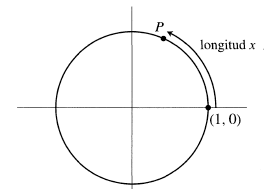
\includegraphics{./img/1.png}
					\end{center}

					Por definición $L(x_1, x_2)$ nos da la longitud de arco de $(x_1, x_2)$ a $(1, 0)$ si $x_2 \geq 0$ y si $x_2 < 0$ obtenemos la longitud de arco de $(x_1, x_2)$ a $(1, 0)$ en sentido horario asi que al sumar $\pi$ obtenemos el sentido deseado.

					Para definir $d(x, y)$ tomemos $L(x_1, x_2)$ y $L(y_1, y_2)$ y nos fijamos en su diferencia (Al rastro negro le quitamos el rastro morado)

					\begin{center}
						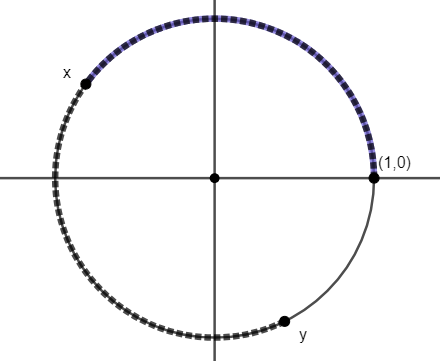
\includegraphics{./img/2.png}
					\end{center}

					Esto es, $d(x, y) := \abs{L(x_1, x_2) - L(y_1, y_2)}$. Observemos que si $d_E$ denota a la métrica Euclidiana, entonces $d(x, y) = \abs{L(x_1, x_2) - L(y_1, y_2)} = \abs{L(x) - L(y)} = d_E(L(x), L(y))$ además $L$ es inyectiva, pues $arcos$ lo es asi que de la Proposicion anterior tenemos que $(M, d)$ es un espacio métrico \qed

				\end{proof}
			
			\end{Ejemplos}

			\begin{Proposicion}\setlength{\parindent}{0em}
				
				Sean $(M, d)$ un espacio métrico y $d' : M \times M \to M$ tal que para cualesquiera $x, y \in M$, $d'(x, y) = \min\{ 1, d(x, y) \}$, entonces $(M, d')$ es un espacio métrico.

				\begin{proof}
					
					Sean $(M, d)$ un espacio métrico y $d' : M \times M \to M$ tal que para cualesquiera $x, y \in M$, $d'(x, y) = \min\{ 1, d(x, y) \}$ \\
					\pd $(M, d')$ es un espacio métrico

					Sean $x, y, z \in M$, observemos que si $d(x, y) = 0$, entonces $d'(x, y) = \min\{ 1, d(x, y) \} = \min\{ 1, 0 \} = 0$, es decir $d(x, y) = 0 \Rightarrow d'(x, y) = 0$ pero tambien si $d'(x, y) = 0$, entonces $\min\{ 1, d(x, y) \} = 0$ por lo que $0 = d(x, y)$ asi que $d'(x, y) = 0 \Rightarrow d(x, y) = 0$ por tanto $d'(x, y) = 0 \Leftrightarrow d(x, y) = 0$ de donde 

					\[ x = y \Leftrightarrow d(x, y) = 0 \Leftrightarrow d'(x, y) = 0 \]

					Asi que $x = y \Leftrightarrow d'(x, y) = 0$. Note que $1, d(x, y) \geq 0$ asi que $\min\{ 1, d(x, y) \} \geq 0$ por lo que $d'(x, y) \geq 0$. Para probar la desigualdad triangular procederemos por casos

					\textbf{a)} $\min\{ 1, d(x, y) \} = 1$ \\
					Entonces tenemos dos subcasos

					\indentar{1cm}{
					
						\textbf{a).1)} $\min\{ 1, d(x, z) \} = 1$ \\
						Tenemos que $0 \leq d'(y, z)$ asi que $1 \leq 1 + d'(y, z)$ o sea que $\min\{ 1, d(x, y) \} \leq \min\{ 1, d(x, z) \} + d'(y, z)$ es decir $d'(x, y) \leq d'(x, z) + d'(y, z)$.

						\textbf{a).2)} $\min\{ 1, d(x, z) \} = d(x, z)$ \\
						Tenemos otros dos subcasos 

						\indentar{1.5cm}{

							\textbf{a).2).I)} $\min\{ 1, d(y, z) \} = 1$ \\
							Tenemos que $0 \leq d'(x, z)$ por lo que $1 \leq d'(x, z) + 1$ es decir $\min\{ 1, d(x, y) \} \leq d'(x, z) + \min\{ 1, d(y, z) \}$ por tanto $d'(x, y) \leq d'(x, z) + d'(y, z)$.

							\textbf{a).2).II)} $\min\{ 1, d(y, z) \} = d(y, z)$ \\
							Tenemos que $d'(x, y) = 1 \leq d(x, y) \leq d(x, z) + d(y, z) = \min\{ 1, d(x, z) \} + \min\{ 1, d(y, z) \} = d'(x, z) + d'(y, z)$ por tanto $d'(x, y) \leq d'(x, z) + d'(y, z)$.
					
						}

						En ambos subcasos $d'(x, y) \leq d'(x, z) + d'(y, z)$

					}

					En los dos subcasos obtenemos que $d'(x, y) \leq d'(x, z) + d'(y, z)$.

					\textbf{b)} $\min\{ 1, d(x, y) \} = d(x, y)$ \\
					Entonces tenemos dos subcasos
					
					\indentar{1cm}{

						\textbf{b).1)} $\min\{ 1, d(x, z) \} = 1$ \\
						En este caso tenemos que $d'(x, y) = \min\{ 1, d(x, y) \} = d(x, y) \leq 1 \leq 1 + d'(y, z) = \min\{ 1, d(x, z) \} + d'(y, z) = d'(x, z) + d'(y, z)$ por tanto $d'(x, y) \leq d'(x, z) + d'(y, z)$

						\textbf{b).2)} $\min\{ 1, d(x, z) \} = d(x, z)$ \\
						Tenemos otros dos subcasos 

						\indentar{1.5cm}{

							\textbf{b).2).I)} $\min\{ 1, d(y, z) \} = 1$ \\
							Entonces $d'(x, y) = \min\{ 1, d(x, y) \} = d(x, y) \leq 1 \leq d(x, z) + 1 = \min\{ 1, d(x, z) \} + \min\{ 1, d(y, z) \} = d'(x, z) + d'(y, z)$ por tanto $d'(x, y) \leq d'(x, z) + d'(y, z)$

							\textbf{b).2).II)} $\min\{ 1, d(y, z) \} = d(y, z)$ \\
							Entonces $d'(x, y) = \min\{ 1, d(x, y) \} = d(x, y) \leq d(x, z) + d(y, z) = \min\{ 1, d(x, z) \} + \min\{ 1, d(y, z) \} = d'(x, z) + d'(y, z)$ por tanto $d'(x, y) \leq d'(x, z) + d'(y, z)$ 

						}

						En ambos subcasos $d'(x, y) \leq d'(x, z) + d'(y, z)$

					}

					En los dos subcasos obtenemos que $d'(x, y) \leq d'(x, z) + d'(y, z)$.

					De este modo tanto en \textbf{a)} como en \textbf{b)} obtenemos que $d'(x, y) \leq d'(x, z) + d'(y, z)$ por tanto $(M, d')$ es un espacio métrico \qed

				\end{proof}

			\end{Proposicion}

			\begin{Teorema}\setlength{\parindent}{0em}
				
				Sea $(F, \rho)$ un espacio pseudométrico, definimos la relación $\sim$  en $F$ como sigue, para cualesquiera $x, y \in F$, $x \sim y$ si y sólo si $\rho(x, y) = 0$, entonces 
				
				\textbf{1)} $\sim$ es una relación de equivalencia 
				
				\textbf{2)} Si $x \sim y$ y $z \sim w$, entonces $\rho(x, z) = \rho(y, w)$ 

				\textbf{3)} Si $M = F/\sim$, para cualesquiera $\alpha, \beta \in M$ tomamos $x \in \alpha$, $y \in \beta$ y definimos $d(\alpha, \beta) := \rho(x, y)$, entonces $(M, d)$ es un espacio métrico 

				\begin{proof}
					
					Sean $(F, \rho)$ un espacio pseudométrico y $x, y, z, w \in F$, definimos la relación $\sim$  en $F$ como sigue, para cualesquiera $x_1, x_2 \in F$, $x_1 \sim x_2$ si y sólo si $\rho(x_1, x_2) = 0$ \\
					\pd \textbf{1) - 3)}

					\textbf{1)} \pd $\sim$ es una relación de equivalencia \\
					Tenemos que $\rho(x, x) = 0$ por lo que $x \sim x$. Por otro lado si $x \sim y$ entonces $\rho(x, y) = 0$ pero $\rho(x, y) = \rho(y, x)$ asi que $\rho(y, x) = 0$ en consecuencia $y \sim x$. Finalmente si $x \sim y$ y $y \sim z$ entonces $\rho(x, y) = 0 = \rho(y, z)$ por lo que $\rho(x, z) \leq \rho(x, y) + \rho(y, z) = 0 + 0 = 0$ de modo que $\rho(x, z) = 0$ luego $x \sim z$ por tanto $\sim$ es relación de equivalencia.
					
					\textbf{2)} Supongamos que $x \sim y$ y $z \sim w$ \\
					\pd $\rho(x, z) = \rho(y, w)$ \\
					Tenemos que $\rho(x, y) = 0$ y $\rho(z, w) = 0$ asi que por el Lema \ref{Lema: Primer lema de metricas} tenemos que $\abs{\rho(x, z) - \rho(y, w)} \leq d(x, y) + d(z, w) = 0 + 0 = 0$ por lo que $\abs{\rho(x, z) - \rho(y, w)} \leq 0$ luego $\rho(x, z) - \rho(y, w) = 0$ por tanto $\rho(x, z) = \rho(y, w)$ \\

					\textbf{3)} Sea $M = F/\sim$ para cualesquiera $\alpha, \beta \in M$ tomamos $x \in \alpha$, $y \in \beta$ y definimos $d(\alpha, \beta) := \rho(x, y)$ \\
					\pd $(M, d)$ es un espacio métrico \\
					Observemos que $d$ esta bien definida por los incisos \textbf{1)} y \textbf{2)}, ahora tomemos $\alpha, \beta, \gamma \in M$ y $a \in \alpha, b \in \beta$ y $c \in \gamma$. Veamos que $d$ satisface los puntos de la definición de espacio métrico

					\indentar{1cm}{

						\textbf{3).a)} \pd $d(\alpha, \alpha) = 0$ \\
						Tenemos que $d(\alpha, \alpha) = \rho(a, a) = 0$ por tanto $d(\alpha, \alpha) = 0$

						\textbf{3).b)} Sup. $\alpha \neq \beta$ \\
						\pd $d(\alpha, \beta) > 0$ \\
						Si $d(\alpha, \beta) = 0$ entonces $\rho(a, b) = 0$ luego $a \sim b$ por lo que $\alpha \n \beta \neq \emptyset$ y como $\sim$ es de equivalencia, tenemos que $\alpha = \beta$ \c por tanto $d(\alpha, \beta) > 0$

						\textbf{3).c)} \pd $d(\alpha, \beta) = d(\beta, \alpha)$ \\
						Tenemos que $d(\alpha, \beta) = \rho(a, b) = \rho(b, a) = d(\beta, \alpha)$ por tanto  $d(\alpha, \beta) = d(\beta, \alpha)$
						
						\textbf{3).d)} \pd $d(\alpha, \beta) \leq d(\alpha, \gamma) + d(\gamma, \beta)$ \\
						Se tiene que $d(\alpha, \beta) = \rho(a, b) \leq \rho(a, c) + \rho(c, b) = d(\alpha, \gamma) + d(\gamma, \beta)$ por tanto $d(\alpha, \beta) \leq d(\alpha, \gamma) + d(\gamma, \beta)$

					}

					De \textbf{3).a) - 3).d)} tenemos que $(M, d)$ es un espacio métrico \qed

				\end{proof}

			\end{Teorema}

			\begin{Teorema}\setlength{\parindent}{0em}
				
				Sean $M \neq \emptyset$ y $d_1, d_2, ..., d_n$ métricas sobre $M$, definimos $d' : M \times M \to M$ como sigue, para cualesquiera $x_1, x_2 \in M$, $d'(x_1, x_2) = \sum_{i = 1}^{n} d_i(x_1, x_2)$, entonces $(M, d')$ es un espacio métrico. 

				\begin{proof}
					
					Sean $M \neq \emptyset$, $x, y, z \in M$ y $d_1, d_2, ..., d_n$ métricas sobre $M$, definimos $d' : M \times M \to M$ como sigue, para cualesquiera $x, y \in M$, $d'(x, y) = \sum_{i = 1}^{n} d_i(x, y)$ \\
					\pd $(M, d')$ es un espacio métrico

					\textbf{1)} \pd $x = y \Leftrightarrow d'(x, y) = 0$ \\
					\necesidad Sup. $x = y$ \\
					\pd $d'(x, y) = 0$ \\
					Como $x = y$ entonces $d_1(x, y) = d_2(x, y) = ... = d_n(x, y) = 0$ por lo que $d'(x, y) = \sum_{i = 1}^{n} d_i(x, y) = \sum_{i = 1}^{n} 0 = 0$ por tanto $d'(x, y) = 0$

					\suficiencia Sup. $d'(x, y) = 0$ \\
					\pd $x = y$
					Como $d'(x, y) = 0$ tenemos que $\sum_{i = 1}^{n} d_i(x, y) = 0$ pero como todos los sumandos son mayores o iguales que cero, esto implica que cada sumando es cero, en particular $d_1(x, y) = 0$ luego $x = y$

					\textbf{2)} \pd $d'(x, y) \leq d'(x, z) + d'(y, z)$ \\
					Para cada $i \in \{ 1, 2, ..., n \}$ tenemos que $d_i(x, y) \leq d_i(x, z) + d_i(y, z)$ por lo que $d'(x, y) = \sum_{i = 1}^{n} d_i(x, y) \leq \sum_{i = 1}^{n} \left( d_i(x, z) + d_i(y, z) \right) = \sum_{i = 1}^{n} d_i(x, z) + \sum_{i = 1}^{n} d_i(y, z) = d'(x, z) + d'(y, z)$ por tanto $d'(x, y) \leq d'(x, z) + d'(y, z)$

					Por \textbf{1)} y \textbf{2)} podemos concluir que $(M, d')$ es un espacio métrico \qed

				\end{proof}

			\end{Teorema}

			\begin{Teorema}\label{Teorema: Metrica a partir de otra, fraccion con denominador 1 mas la metrica}\setlength{\parindent}{0em}
				
				Sean $(M, d)$ un espacio métrico y $d' : M \times M \to M$ tal que para cualesquiera $x, y \in M$, $d'(x, y) = \frac{d(x,y)}{1 + d(x, y)}$, entonces $(M, d')$ es un espacio métrico. 

				\begin{proof}
					
					Sean $(M, d)$ un espacio métrico, $x, y, z \in M$ y $d' : M \times M \to M$ tal que para cualesquiera $x_1, x_2 \in M$, $d'(x_1, x_2) = \frac{d(x_1,x_2)}{1 + d(x_1, x_2)}$ \\
					\pd $(M, d')$ es un espacio métrico

					Tenemos que
					
					\[ d'(x, y) = 0 \Leftrightarrow \frac{d(x, y)}{1 + d(x, y)} = 0 \Leftrightarrow d(x, y) = 0 \Leftrightarrow x = y \]

					Por tanto $x = y \Leftrightarrow d'(x, y) = 0$. Por otro lado observe que por ser cada factor mayor o igual que cero, tenemos que: 

					$0 \leq 2d(x, z)d(y, z) + d(x, y)d(x, z)d(y, z)$ \\
					\Imp $0 \leq 2d(x, z)d(y, z) + d(x, y)d(x, z)d(y, z)$ \\
					\Imp $d(x, y) \leq d(x, z) + d(y, z) + 2d(x, z)d(y, z) + d(x, y)d(x, z)d(y, z)$ (Pues $d(x, y) \leq d(x, z) + d(y, z)$) \\
					\Imp $d(x, y) + d(x, y)d(x, z) + d(x, y)d(y, z) + d(x, y)d(x, z)d(y, z) \leq d(x, z) + d(y, z) + 2d(x, z)d(y, z) + d(x, y)d(x, z)d(y, z) + d(x, y)d(x, z) + d(x, y)d(y, z) + d(x, y)d(x, z)d(y, z)$ \\
					\Imp $d(x, y) + d(x, y)d(x, z) + d(x, y)d(y, z) + d(x, y)d(x, z)d(y, z) \leq d(x, z) + d(y, z) + 2d(x, z)d(y, z) + d(x, y)d(x, z) + d(x, y)d(y, z) + d(x, y)d(x, z)d(y, z) + d(x, y)d(x, z)d(y, z)$ \\
					\Imp $d(x, y) + d(x, y)d(x, z) + d(x, y)d(y, z) + d(x, y)d(x, z)d(y, z) \leq d(x, z) + d(y, z) + 2d(x, z)d(y, z) + d(x, y)d(x, z) + d(x, y)d(y, z) + 2d(x, y)d(x, z)d(y, z)$ \\
					\Imp $d(x, y)(1 + d(x, z) + d(y, z) + d(x, z)d(y, z)) \leq d(x, z) + d(y, z) + 2d(x, z)d(y, z) + d(x, y)d(x, z) + d(x, y)d(y, z) + 2d(x, y)d(x, z)d(y, z)$ \\
					\Imp $d(x, y)(1 + d(x, z))(1 + d(y, z)) \leq d(x, z) + d(y, z) + 2d(x, z)d(y, z) + d(x, y)d(x, z) + d(x, y)d(y, z) + 2d(x, y)d(x, z)d(y, z)$ \\
					\Imp $d(x, y)(1 + d(x, z))(1 + d(y, z)) \leq (1 + d(x, y))(d(x, z) + d(y, z) + 2d(x, z)d(y, z))$ \\
					\Imp $d(x, y) \leq \frac{(1 + d(x, y))(d(x, z) + d(y, z) + 2d(x, z)d(y, z))}{(1 + d(x, z))(1 + d(y, z))}$ \\
					\Imp $\frac{d(x, y)}{1 + d(x, y)} \leq \frac{d(x, z) + d(y, z) + 2d(x, z)d(y, z)}{(1 + d(x, z))(1 + d(y, z))}$ \\
					\Imp $d'(x, y) \leq \frac{d(x, z) + d(y, z) + 2d(x, z)d(y, z)}{(1 + d(x, z))(1 + d(y, z))}$ \\
					\Imp $d'(x, y) \leq \frac{d(x, z) + 2d(x, z)d(y, z) + d(y, z)}{(1 + d(x, z))(1 + d(y, z))}$ \\
					\Imp $d'(x, y) \leq \frac{d(x, z) + d(x, z)d(y, z) + d(x, z)d(y, z) + d(y, z)}{(1 + d(x, z))(1 + d(y, z))}$ \\
					\Imp $d'(x, y) \leq \frac{d(x, z)(1 + d(y, z)) + d(y, z)(1 + d(x, z))}{(1 + d(x, z))(1 + d(y, z))}$ \\
					\Imp $d'(x, y) \leq \frac{d(x, z)}{1 + d(x, z)} + \frac{d(y, z)}{1 + d(y, z)}$ \\
					\Imp $d'(x, y) \leq d'(x, z) + d'(y, z)$

					Por lo tanto $(M, d')$ es un espacio métrico \qed

				\end{proof}

			\end{Teorema}

			\begin{Teorema}\setlength{\parindent}{0em}
				
				Sean $(M, d_M), (S, d_S)$ espacios métricos, para cualesquiera $x = (x_1, x_2), y = (y_1, y_2) \in M \times S$ definimos $d_{M \times S}(x, y) := d_M(x_1, y_1) + d_S(x_2, y_2)$, entonces $d_{M \times S}$ es una métrica para $M \times S$.

				\begin{proof}
					
					Sean $(M, d_M), (S, d_S)$ espacios métricos, para cualesquiera $x = (x_1, x_2), y = (y_1, y_2) \in M \times S$ definimos $d_{M \times S}(x, y) := d_M(x_1, y_1) + d_S(x_2, y_2)$ \\ \pd $d_{M \times S}$ es una métrica para $M \times S$.

					Sean $x, y, z \in M \times S$ tales que $x = (x_1, x_2), y = (y_1, y_2), z = (z_1, z_2)$, observemos que $d_{M \times S}(x, y) = 0 \Leftrightarrow d_M(x_1, y_1) + d_S(x_2, y_2) = 0 \Leftrightarrow d_M(x_1, y_1) = 0 = d_S(x_2, y_2) \Leftrightarrow x_1 = y_1 \y x_2 = y_2 \Leftrightarrow (x_1, x_2) = (y_2, y_2) \Leftrightarrow x = y$ por tanto $x = y \Leftrightarrow d_{M \times S}(x, y) = 0$.

					Por otro lado $d_{M \times S}(x, y) = d_M(x_1, y_1) + d_S(x_2, y_2) \leq (d_M(x_1, z_1) + d_M(y_1, z_1)) + (d_S(x_2, z_2) + d_S(y_2, z_2)) = (d_M(x_1, z_1) + d_S(x_2, z_2)) + (d_M(y_1, z_1) + d_S(y_2, z_2)) = d_{M \times S}(x, z) + d_{M \times S}(y, z)$ por tanto $d_{M \times S}(x, y) \leq d_{M \times S}(x, z) + d_{M \times S}(y, z)$ luego $d_{M \times S}$ es una métrica para $M \times S$ \qed

				\end{proof}

			\end{Teorema}

			\begin{Teorema}\setlength{\parindent}{0em}
				
				Sean $(M, d_M), (S, d_S)$ espacios métricos, para cualesquiera $x = (x_1, x_2), y = (y_1, y_2) \in M \times S$ definimos $d'(x, y) := \max\{ d_M(x_1, y_1), d_S(x_2, y_2) \}$, entonces $d'$ es una métrica para $M \times S$.

				\begin{proof}
					
					Sean $(M, d_M), (S, d_S)$ espacios métricos, para cualesquiera $x = (x_1, x_2), y = (y_1, y_2) \in M \times S$ definimos $d'(x, y) := \max\{ d_M(x_1, y_1), d_S(x_2, y_2) \}$ \\
					\pd $d'$ es una métrica para $M \times S$.

					Sean $x, y, z \in M \times S$ tales que $x = (x_1, x_2), y = (y_1, y_2), z = (z_1, z_2)$, observemos que $d'(x, y) = 0 \Leftrightarrow \max\{ d_M(x_1, y_1), d_S(x_2, y_2) \} = 0 \Leftrightarrow d_M(x_1, y_1) = 0 = d_S(x_2, y_2) \Leftrightarrow x_1 = y_1 \y x_2 = y_2 \Leftrightarrow (x_1, x_2) = (y_2, y_2) \Leftrightarrow x = y$ por tanto $x = y \Leftrightarrow d'(x, y) = 0$.

					Para probar la desigualdad triangular procedamos por casos:

					\textbf{1)} $\max\{ d_M(x_1, y_1), d_S(x_2, y_2) \} = d_M(x_1, y_1)$ \\
					Entonces $d'(x, y) = \max\{ d_M(x_1, y_1), d_S(x_2, y_2) \} = d_M(x_1, y_1) \leq d_M(x_1, z_1) + d_M(y_1, z_1)$ \\ $\leq \max\{ d_M(x_1, z_1), d_S(x_2, z_2) \} + \max\{ d_M(y_1, z_1), d_S(y_2, z_2) \} = d'(x, z) + d'(y, x)$ por tanto $d'(x, y) \leq d'(x, z) + d'(y, z)$.

					\textbf{2)} $\max\{ d_M(x_1, y_1), d_S(x_2, y_2) \} = d_S(x_2, y_2)$ \\
					Entonces $d'(x, y) = \max\{ d_M(x_1, y_1), d_S(x_2, y_2) \} = d_S(x_2, y_2) \leq d_S(x_2, z_2) + d_S(y_2, z_2)$ \\ $\leq \max\{ d_M(x_1, z_1), d_S(x_2, z_2) \} + \max\{ d_M(y_1, z_1), d_S(y_2, z_2) \} = d'(x, z) + d'(y, x)$ por tanto $d'(x, y) \leq d'(x, z) + d'(y, z)$.

					En ambos casos $d'(x, y) \leq d'(x, z) + d'(y, z)$ por tanto $d'$ es una métrica para $M \times S$ \qed

				\end{proof}

			\end{Teorema}

			\begin{Teorema}\setlength{\parindent}{0em}
				
				Sean $(M, d_M), (S, d_S)$ espacios métricos, para cualesquiera $x = (x_1, x_2), y = (y_1, y_2) \in M \times S$ definimos $d'(x, y) := \sqrt{d_M(x_1, y_1)^2 + d_S(x_2, y_2)^2}$, entonces $d'$ es una métrica para $M \times S$.

				\begin{proof}
					
					Sean $(M, d_M), (S, d_S)$ espacios métricos, para cualesquiera $x = (x_1, x_2), y = (y_1, y_2) \in M \times S$ definimos $d'(x, y) := \sqrt{d_M(x_1, y_1)^2 + d_S(x_2, y_2)^2}$ \\
					\pd $d'$ es una métrica para $M \times S$.

					Sean $x, y, z \in M \times S$ tales que $x = (x_1, x_2), y = (y_1, y_2), z = (z_1, z_2)$, observemos que $d'(x, y) = 0 \Leftrightarrow \sqrt{d_M(x_1, y_1)^2 + d_S(x_2, y_2)^2} = 0 \Leftrightarrow d_M(x_1, y_1)^2 + d_S(x_2, y_2)^2 = 0 \Leftrightarrow d_M(x_1, y_1)^2 = 0 = d_S(x_2, y_2)^2 \Leftrightarrow d_M(x_1, y_1) = 0 = d_S(x_2, y_2) \Leftrightarrow x_1 = y_1 \y x_2 = y_2 \Leftrightarrow (x_1, x_2) = (y_2, y_2) \Leftrightarrow x = y$ por tanto $x = y \Leftrightarrow d'(x, y) = 0$.

					Ahora veamos que si $a, b, c, d \in \R_{+} \u \{ 0 \}$, $a \leq b$ y $c \leq d$, entonces $\norm{(a, c)} \leq \norm{(b, d)}$. Tenemos que $a^2 \leq b^2$ y $c^2 \leq d^2$ luego $a^2 + c^2 \leq b^2 + d^2$ asi que $\sqrt{a^2 + c^2} \leq \sqrt{b^2 + d^2}$ es decir $\norm{(a, c)} \leq \norm{(b, d)}$. Como caso particular tenemos que, como $d_M(x_1, y_1) \leq d_M(x_1, z_1) + d_M(y_1, z_1)$ y $d_S(x_2, y_2) \leq d_S(x_2, z_2) + d_S(y_2, z_2)$ entonces 
					
					\begin{equation}\tag{$\star$}
						\norm{(d_M(x_1, y_1), d_S(x_2, y_2))} \leq \norm{(d_M(x_1, z_1) + d_M(y_1, z_1), d_S(x_2, z_2) + d_S(y_2, z_2))}
					\end{equation}
					
					Por otro lado notemos que:
					
					$d'(x, z) + d'(y, z) = \sqrt{d_M(x_1, z_1)^2 + d_S(x_2, z_2)^2} + \sqrt{d_M(y_1, z_1)^2 + d_S(y_2, z_2)^2}$ \\
					$= \norm{(d_M(x_1, z_1), d_S(x_2, z_2))} + \norm{(d_M(y_1, z_1), d_S(y_2, z_2))}$ \\
					$\geq \norm{(d_M(x_1, z_1), d_S(x_2, z_2)) + (d_M(y_1, z_1), d_S(y_2, z_2))}$ \\
					$= \norm{(d_M(x_1, z_1) + d_M(y_1, z_1), d_S(x_2, z_2) + d_S(y_2, z_2))}$ \\
					$\geq \norm{(d_M(x_1, y_1), d_S(x_2, y_2))}$
					$= d'(x, y)$ \hspace{3cm} (Por $\star$)

					Por tanto $d'(x, y) \leq d'(x, z) + d'(y, z)$ luego $d'$ es una métrica para $M \times S$ \qed

				\end{proof}

			\end{Teorema}

			\begin{Teorema}\setlength{\parindent}{0em}
				
				Sean $M \neq \emptyset$ y $\{ d_n \}$ una sucesión de métricas para $M$ tales que 

				\[ \forall x, y \in M : \forall n \in \mathbb{N} : d_n(x, y) \leq 1 \] 

				Entonces $d' = \displaystyle\sum_{n = 0}^{\infty} \frac{d_n}{2^n}$ es una métrica sobre $M$. 

				\begin{proof}
					
					Sean $M \neq \emptyset$ y $\{ d_n \}$ una sucesión de métricas para $M$ tales que $\forall x, y \in M : \forall n \in \mathbb{N} : d_n(x, y) \leq 1$. Definimos $d' = \sum_{n = 0}^{\infty} \frac{d_n}{2^n}$ \\
					\pd $d'$ es una métrica sobre $M$

					Sean $x, y, z \in M$,veamos que $d'(x, y) = 0 \Leftrightarrow x = y$ y que $d'(x, y) \leq d'(x, z) + d'(y, z)$ 

					\textbf{a)} \pd $d'(x, y) = 0 \Leftrightarrow x = y$ \\
					\necesidad Sup. $d'(x, y) = 0$ \\
					\pd $x = y$ \\
					Si $x \neq y$, entonces para cada $d_n$ de la sucesión $\{ d_n \}$ tenemos que $d_n(x, y) > 0$ asi que $\frac{d_n(x, y)}{2^n} > 0$ luego $\sum_{i = 0}^{n} \frac{d_i(x, y)}{2^i} > 0$ por lo que $\sum_{n = 0}^{\infty} \frac{d_n(x, y)}{2^n} > 0$ es decir $d'(x, y) > 0$ \c por tanto $x = y$

					\suficiencia Sup. $x = y$ \\
					\pd $d'(x, y) = 0$ \\
					Para cada $d_n$ de la sucesión $\{ d_n \}$ tenemos que $d_n(x, y) = 0$ asi que $\frac{d_n(x, y)}{2^n} = 0$ luego $\sum_{i = 0}^{n} \frac{d_i(x, y)}{2^i} = 0$ por lo que $\sum_{n = 0}^{\infty} \frac{d_n(x, y)}{2^n} = 0$ es decir $d'(x, y) = 0$.

					\textbf{b)} \pd $d'(x, y) \leq d'(x, z) + d'(y, z)$ \\
					Para cada $d_n$ de la sucesión $\{ d_n \}$ tenemos que $d_n(x, y) \leq d_n(x, z) + d_n(y, z)$ asi que $\frac{d_n(x, y)}{2^n} \leq \frac{d_n(x, z) + d_n(y, z)}{2^n}$ luego $\sum_{i = 0}^{n} \frac{d_i(x, y)}{2^i} \leq \sum_{i = 0}^{n} \frac{d_i(x, z) + d_i(y, z)}{2^i}$ asi que $d'(x, y) = \sum_{n = 0}^{\infty} \frac{d_n(x, y)}{2^n} \leq \sum_{n = 0}^{\infty} \frac{d_n(x, z) + d_n(y, z)}{2^n} = \sum_{n = 0}^{\infty} \frac{d_n(x, z)}{2^n} + \sum_{n = 0}^{\infty} \frac{d_n(y, z)}{2^n} = d'(x, z) + d'(y, z)$ por tanto $d'(x, y) \leq d'(x, z) + d'(y, z)$ 

					De \textbf{a)} y \textbf{b)} podemos concluir que $d'$ es una métrica para $M$ \qed


				\end{proof}

			\end{Teorema}

		\section{Métricas relacionadas con $\R$}

			\begin{Teorema}\setlength{\parindent}{0em}
				
				Sea $M$ el conjunto de todas las sucesiones reales acotadas y $d : M \times M \to \R$ tal que para cualesquiera $\{ x_n \}, \{ y_n \} \in M$, $d(\{ x_n \}, \{ y_n \}) = \sup\{ \abs{ x_n - y_n} : n \in N \}$, entonces $(M, d)$ es un espacio métrico.

				\begin{proof}
					
					Sea $M$ el conjunto de todas las sucesiones reales acotadas y $d : M \times M \to M$ tal que para cualesquiera $\{ x_n \}, \{ y_n \} \in M$, $d(\{ x_n \}, \{ y_n \}) = \sup\{ \abs{x_n - y_n} : n \in N \}$ \\
					\pd $(M, d)$ es un espacio métrico

					Observemos que $M = B(\Z_{+})$ asi que por los Ejemplos \ref{Ejemplos: Metricas basicas} inciso 7 directamente tenemos que $(B(\Z_{+}), d) = (M, d)$ es un espacio métrico \qed

				\end{proof}

			\end{Teorema}

			\begin{Teorema}\setlength{\parindent}{0em}
				
				Sea $M$ el conjunto de todas las sucesiones reales y $d : M \times M \to M$ tal que para cualesquiera $\{ x_n \}, \{ y_n \} \in M$, $d(\{ x_n \}, \{ y_n \}) = \sum_{n = 0}^{\infty} \frac{1}{n!} \cdot \frac{\abs{x_n - y_n}}{1 + \abs{x_n - y_n}}$, entonces $(M, d)$ es un espacio métrico. 

				\begin{proof}
					
					Sea $M$ el conjunto de todas las sucesiones reales, definimos $d : M \times M \to M$ tal que para cualesquiera $\{ x_n \}, \{ y_n \} \in M$, $d(\{ x_n \}, \{ y_n \}) = \sum_{n = 0}^{\infty} \frac{1}{n!} \cdot \frac{\abs{x_n - y_n}}{1 + \abs{x_n - y_n}}$ \\
					\pd $(M, d)$ es un espacio métrico

					Sean $\{ x_n \}, \{ y_n \}, \{ z_n \} \in M$, veamos que $d(\{ x_n \}, \{ y_n \}) = 0 \Leftrightarrow \{ x_n \} = \{ y_n \}$ y $d(\{ x_n \}, \{ y_n \}) \leq d(\{ x_n \}, \{ z_n \}) + d(\{ y_n \}, \{ z_n \})$

					\textbf{a)} \pd $d(\{ x_n \}, \{ y_n \}) = 0 \Leftrightarrow \{ x_n \} = \{ y_n \}$ \\
					\necesidad Sup. $d(\{ x_n \}, \{ y_n \}) = 0$ \\
					\pd $\{ x_n \} = \{ y_n \}$ \\
					Si $\{ x_n \} \neq \{ y_n \}$ entonces existe un término donde las sucesiones no coinciden, estos es, existe un $m \in \Z_{+}$ tal que $x_m \neq y_m$ asi que $\abs{x_m - y_m} \neq 0$ por lo que la suma parcial $\sum_{n = 0}^{m} \frac{1}{n!} \cdot \frac{\abs{x_n - y_n}}{1 + \abs{x_n - y_n}} > 0$ y el resto de sumas parciales son mayores o iguales a cero, por lo que $\sum_{n = 0}^{\infty} \frac{1}{n!} \cdot \frac{\abs{x_n - y_n}}{1 + \abs{x_n - y_n}} > 0$ \c por tanto $\{ x_n \} = \{ y_n \}$

					\suficiencia Sup. $\{ x_n \} = \{ y_n \}$ \\
					\pd $d(\{ x_n \}, \{ y_n \}) = 0$ \\
					Tenemos que $d(\{ x_n \}, \{ y_n \}) = \sum_{n = 0}^{\infty} \frac{1}{n!} \cdot \frac{\abs{x_n - y_n}}{1 + \abs{x_n - y_n}} = \sum_{n = 0}^{\infty} \frac{1}{n!} \cdot \frac{\abs{x_n - x_n}}{1 + \abs{x_n - x_n}} = \sum_{n = 0}^{\infty} \frac{1}{n!} \cdot \frac{0}{1 + 0} = \sum_{n = 0}^{\infty} \frac{1}{n!} \cdot 0 = \sum_{n = 0}^{\infty} 0 = 0$ por tanto $d(\{ x_n \}, \{ y_n \}) = 0$

					\textbf{b)} \pd $d(\{ x_n \}, \{ y_n \}) \leq d(\{ x_n \}, \{ z_n \}) + d(\{ y_n \}, \{ z_n \})$ \\
					Sean $x_m, y_m, z_m$ terminos cualesquiera de $\{ x_n \}, \{ y_n \}$ y $\{ z_n \}$ respectivamente. Como $(\R, \absSymbol)$ es un espacio métrico, por el Teorema \ref{Teorema: Metrica a partir de otra, fraccion con denominador 1 mas la metrica} tenemos que 

					\[ \frac{\abs{x_m - y_m}}{1 + \abs{x_m - y_m}} \leq \frac{\abs{x_m - z_m}}{1 + \abs{x_m - z_m}} + \frac{\abs{y_m - z_m}}{1 + \abs{y_m - z_m}} \]

					En consecuencia

					\[ \frac{1}{m!} \cdot \frac{\abs{x_m - y_m}}{1 + \abs{x_m - y_m}} \leq \frac{1}{m!} \cdot \frac{\abs{x_m - z_m}}{1 + \abs{x_m - z_m}} + \frac{\abs{y_m - z_m}}{1 + \abs{y_m - z_m}} \]

					Pero como los terminos de las respectivas sucesiones fueron arbitrarios, entonces para cada $m \in \Z_{+}$ se cumple que 

					\[ \sum_{n = 0}^{m} \frac{1}{n!} \cdot \frac{\abs{x_n - y_n}}{1 + \abs{x_n - y_n}} \leq \sum_{n = 0}^{m} \frac{1}{n!} \cdot \frac{\abs{x_n - z_n}}{1 + \abs{x_n - z_n}} + \sum_{n = 0}^{m} \frac{\abs{y_n - z_n}}{1 + \abs{y_n - z_n}} \]

					Por lo que $\sum_{n = 0}^{\infty} \frac{1}{n!} \cdot \frac{\abs{x_n - y_n}}{1 + \abs{x_n - y_n}} \leq \sum_{n = 0}^{\infty} \frac{1}{n!} \cdot \frac{\abs{x_n - z_n}}{1 + \abs{x_n - z_n}} + \sum_{n = 0}^{\infty} \frac{\abs{y_n - z_n}}{1 + \abs{y_n - z_n}}$ es decir $d(\{ x_n \}, \{ y_n \}) \leq d(\{ x_n \}, \{ z_n \}) + d(\{ y_n \}, \{ z_n \})$

					De \textbf{a)} y \textbf{b)} podemos concluir que $(M, d)$ es un espacio métrico \qed

				\end{proof}

			\end{Teorema}

			\begin{Teorema}\setlength{\parindent}{0em}
				
				Sea $C[a, b]$ el conjunto de todas las funciones continuas de valores reales en el intervalo $[a, b]$, para cualesquiera $f, g \in C[a, b]$ definimos 

				\[ d(f, g) = \int_{a}^{b} \frac{\abs{f(x) - g(x)}}{1 + \abs{f(x) - g(x)}} dx \] 

				Entonces $(C[a, b], d)$ es un espacio métrico.
				
				\begin{proof}
					
					Sea $C[a, b]$ el conjunto de todas las funciones continuas de valores reales en el intervalo $[a, b]$, para cualesquiera $f, g \in C[a, b]$ definimos $d(f, g) = \int_{a}^{b} \frac{\abs{f(x) - g(x)}}{1 + \abs{f(x) - g(x)}} dx$ \\
					\pd $(C[a, b], d)$ es un espacio métrico

					Sean $f, g, h \in C[a, b]$, veamos que $d(f, g) = 0 \Leftrightarrow f = g$ y $d(f, g) \leq d(f, h) + d(g, h)$

					\textbf{a)} \pd $d(f, g) = 0 \Leftrightarrow f = g$ \\
					\necesidad Sup. $d(f, g) = 0$ \\
					\pd $f = g$ \\
					Si $f \neq g$, entonces existe un $x_0 \in [a, b]$ tal que $f(x_0) \neq g(x_0)$ por lo que $\abs{f(x_0) - f(x_0)} > 0$ y tambien $\frac{\abs{f(x_0) - g(x_0)}}{1 + \abs{f(x_0) - g(x_0)}} > 0$ por lo que $\int_{a}^{b} \frac{\abs{f(x) - g(x)}}{1 + \abs{f(x) - g(x)}} dx > 0$ es decir $d(f, g) > 0$ \c por tanto $f = g$ 

					\suficiencia Sup. $f = g$ \\
					\pd $d(f, g) = 0$ \\
					$d(f, g) = \int_{a}^{b} \frac{\abs{f(x) - g(x)}}{1 + \abs{f(x) - g(x)}} dx = \int_{a}^{b} \frac{\abs{f(x) - f(x)}}{1 + \abs{f(x) - f(x)}} dx = \int_{a}^{b} \frac{0}{1 + 0} dx = \int_{a}^{b} 0 = 0$ por tanto $d(f, g) = 0$

					\textbf{b)} \pd $d(f, g) \leq d(f, h) + d(g, h)$ \\
					Sean $x \in [a, b]$, entonces como $(\R, \absSymbol)$ es un espacio métrico, por el Teorema \ref{Teorema: Metrica a partir de otra, fraccion con denominador 1 mas la metrica} tenemos que 

					\[ \frac{\abs{f(x) - g(x)}}{1 + \abs{f(x) - g(x)}} \leq \frac{\abs{f(x) - h(x)}}{1 + \abs{f(x) - h(x)}} + \frac{\abs{g(x) - h(x)}}{1 + \abs{g(x) - h(x)}} \]

					En consecuencia $d(f, g) = \int_{a}^{b} \frac{\abs{f(x) - g(x)}}{1 + \abs{f(x) - g(x)}} dx \leq \int_{a}^{b} \frac{\abs{f(x) - h(x)}}{1 + \abs{f(x) - h(x)}} + \frac{\abs{g(x) - h(x)}}{1 + \abs{g(x) - h(x)}} dx = \int_{a}^{b} \frac{\abs{f(x) - h(x)}}{1 + \abs{f(x) - h(x)}} dx + \int_{a}^{b} \frac{\abs{g(x) - h(x)}}{1 + \abs{g(x) - h(x)}} dx = d(f, h) + f(g, h)$ por tanto $d(f, g) \leq d(f, h) + d(g, h)$

					De \textbf{a)} y \textbf{b)} podemos concluir que $(C[a, b], d)$ es un espacio métrico \qed

				\end{proof}

			\end{Teorema}

		\section{Métricas relacionadas con $\Rn$}

			\begin{Teorema}\setlength{\parindent}{0em}
			
				Sea $d : \Rn \times \Rn \to \R$ tal que para cualesquiera $x = (x_1, x_2, ..., x_n), y = (y_1, y_2, ..., y_n) \in \Rn$, $d(x, y) = \abs{x_1 - y_1} + \abs{x_2 - y_2} + ... + \abs{x_n - y_n}$, entonces $(\Rn, d)$ es un espacio métrico.

				\begin{proof}
					
					Sea $d : \Rn \times \Rn \to \R$ tal que para cualesquiera $x = (x_1, x_2, ..., x_n), y = (y_1, y_2, ..., y_n) \in \Rn$, $d(x, y) = \abs{x_1 - y_1} + \abs{x_2 - y_2} + ... + \abs{x_n - y_n}$ \\ 
					\pd $(\Rn, d)$ es un espacio métrico

					Sean $x = (x_1, x_2, ..., x_n), y = (y_1, y_2, ..., y_n), z = (z_1, z_2, ..., z_n) \in \Rn$.

					\textbf{a)} \pd $d(x, y) = 0 \Leftrightarrow x = y$ \\ 
					Tenemos que 

					\begin{align*}
						d(x, y) = 0 & \Leftrightarrow \abs{x_1 - y_1} + \abs{x_2 - y_2} + ... + \abs{x_n - y_n} = 0 \\ 
						& \Leftrightarrow \abs{x_1 - y_1} = \abs{x_2 - y_2} = ... = \abs{x_n - y_n} = 0 \\ 
						& \Leftrightarrow x_1 = y_1, x_2 = y_2, ..., x_n = y_n \\ 
						& \Leftrightarrow (x_1, x_2, ..., x_n) = (y_1, y_2, ..., y_n) \\ 
						& \Leftrightarrow x = y
					\end{align*}

					Por tanto $d(x, y) = 0 \Leftrightarrow x = y$.

					\textbf{b)} \pd $d(x, y) \leq d(x, z) + d(y, z)$ \\ 
					Al aplicar la desigualdad del triangulo $n$ veces tenemos que

					\begin{align*}
						d(x, y) &= \abs{x_1 - y_1} + \abs{x_2 - y_2} + ... + \abs{x_n - y_n} \\ 
						&\leq (\abs{x_1 - z_1} + \abs{y_1 - z_1}) + (\abs{x_2 - z_2} + \abs{y_2 - z_2}) + ... + (\abs{x_n - z_n} + \abs{y_n - z_n}) \\ 
						&= (\abs{x_1 - z_1} + \abs{x_2 - z_2} + ... + \abs{x_n - z_n}) + (\abs{y_1 - z_1} + \abs{y_2 - z_2} + ... + \abs{y_n - z_n}) \\ 
						&= d(x, z) + d(y, z)
					\end{align*}

					Por tanto $d(x, y) \leq d(x, z) + d(y, z)$.

					De \textbf{a)} y \textbf{b)} podemos concluir que $(\Rn, d)$ es un espacio métrico \qed

				\end{proof}
			
			\end{Teorema}

			\begin{Teorema}\setlength{\parindent}{0em}
			
				Sea $d : \Rn \times \Rn \to \R$ tal que para cualesquiera $x = (x_1, x_2, ..., x_n), y = (y_1, y_2, ..., y_n) \in \Rn$, $d(x, y) = \max\{ \abs{x_1 - y_1}, \abs{x_2 - y_2}, ..., \abs{x_n - y_n} \}$, entonces $(\Rn, d)$ es un espacio métrico.

				\begin{proof}
					
					Sea $d : \Rn \times \Rn \to \R$ tal que para cualesquiera $x = (x_1, x_2, ..., x_n), y = (y_1, y_2, ..., y_n) \in \Rn$, $d(x, y) = \max\{ \abs{x_1 - y_1}, \abs{x_2 - y_2}, ..., \abs{x_n - y_n} \}$ \\ 
					\pd $(\Rn, d)$ es un espacio métrico

					Sean $x = (x_1, x_2, ..., x_n), y = (y_1, y_2, ..., y_n), z = (z_1, z_2, ..., z_n) \in \Rn$.

					\textbf{a)} \pd $d(x, y) = 0 \Leftrightarrow x = y$ \\ 
					Tenemos que 

					\begin{align*}
						d(x, y) = 0 & \Leftrightarrow \max\{ \abs{x_1 - y_1}, \abs{x_2 - y_2}, ..., \abs{x_n - y_n} \} = 0 \\ 
						& \Leftrightarrow \abs{x_1 - y_1} = \abs{x_2 - y_2} = ... = \abs{x_n - y_n} = 0 \\ 
						& \Leftrightarrow x_1 = y_1, x_2 = y_2, ..., x_n = y_n \\ 
						& \Leftrightarrow (x_1, x_2, ..., x_n) = (y_1, y_2, ..., y_n) \\ 
						& \Leftrightarrow x = y
					\end{align*}

					Por tanto $d(x, y) = 0 \Leftrightarrow x = y$.

					\textbf{b)} \pd $d(x, y) \leq d(x, z) + d(y, z)$ \\ 
					Tenemos que 

					\begin{align*}
						d(x, y) &= \max\{ \abs{x_1 - y_1}, \abs{x_2 - y_2}, ..., \abs{x_n - y_n} \} \\ 
						&\leq \max\{ \abs{x_1 - z_1} + \abs{y_1 - z_1}, \abs{x_2 - z_2} + \abs{y_2 - z_2}, ..., \abs{x_n - z_n} + \abs{y_n - z_n} \} \\ 
						&\leq \max\{ \abs{x_1 - z_1}, \abs{x_2 - z_2}, ..., \abs{x_n - z_n} \} + \max\{ \abs{y_1 - z_1}, \abs{y_2 - z_2}, ..., \abs{y_n - z_n} \} \\ 
						&= d(x, z) + d(y, z)
					\end{align*}

					Por tanto $d(x, y) \leq d(x, z) + d(y, z)$.

					De \textbf{a)} y \textbf{b)} podemos concluir que $(\Rn, d)$ es un espacio métrico \qed

				\end{proof}
			
			\end{Teorema}

		\section{Distancia entre conjuntos}

			\begin{Definicion}[Distancia de un punto a un conjunto]\setlength{\parindent}{0em}
				
				Sean $(M, d)$ un espacio métrico, $x_0 \in M$ y $S \sc M$ no vacio. La distancia de $x_0$ a $S$, denotada $d(x_0, S)$ es el ínfimo de $\{ d(x_0, x) : x \in S \}$, esto es: 

				\[ d(x_0, S) := \inf\{ d(x_0, x) : x \in S \} \] 

				\begin{Obs}
				
					\textbf{1.} Definimos $d(S, x_0)$ como $d(x_0, S)$, es decir $d(S, x_0) := d(x_0, S) = \inf\{ d(x_0, x) : x \in S \}$. 
				
				\end{Obs}

			\end{Definicion}

			\begin{Proposicion}\setlength{\parindent}{0em}
				
				Sean $(M, d)$ un espacio métrico, $x_0, y_0 \in M$ y $S \sc M$ no vacio, entonces 
				
				\textbf{1)} $d(x_0, S) \geq 0$ 

				\textbf{2)} $x_0 \in S$ \Imp $d(x_0, S) = 0$ 

				\textbf{3)} $\abs{d(x_0, S) - d(y_0, S)} \leq d(x_0, y_0)$ 

				\begin{proof}
					
					Sean $(M, d)$ un espacio métrico, $x_0, y_0 \in M$ y $S \sc M$ no vacio \\
					\pd \textbf{1) - 3)} 

					\textbf{1)} \pd $d(x_0, S) \geq 0$ \\
					Si $d(x_0, S) < 0$, entonces $\inf\{ d(x_0, x) : x \in S \} < 0$ por lo que existe un $x_1 \in S$ tal que $\inf\{ d(x_0, x) : x \in S \} \leq d(x_0, x_1) < 0$ pero por definición $d(x_0, x_1) \geq 0$ \c por tanto $d(x_0, S) \geq 0$

					\textbf{2)} Sup. $x_0 \in S$ \\
					\pd $d(x_0, S) = 0$ \\
					Como $x_0 \in S$, entonces $0 = d(x_0, x_0) \in \{ d(x_0, x) : x \in S \}$ luego $0 \geq \inf\{ d(x_0, x) : x \in S \}$ es decir $0 \geq d(x_0, S)$ pero por \textbf{1)} tambien $d(x_0, S) \geq 0$ por tanto $d(x_0, S) = 0$

					\textbf{3)} \pd $\abs{d(x_0, S) - d(y_0, S)} \leq d(x_0, y_0)$ \\
					Para cada $x \in S$ se cumple que $d(x_0, x) \leq d(x_0, y_0) + d(y_0, x)$ luego $d(x_0, S) = \inf\{ d(x_0, x) : x \in S \} \leq \inf\{ d(x_0, y_0) + d(y_0, x) : x \in S \} \leq \inf\{ d(x_0, y_0) : x \in S \} + \inf\{ d(y_0, x) : x \in S \} = d(x_0, y_0) + d(y_0, S)$ por tanto $d(x_0, S) \leq d(x_0, y_0) + d(y_0, S)$ de donde

					\begin{equation}\tag{$\star$}
						d(x_0, S) - d(y_0, S) \leq d(x_0, y_0)
					\end{equation}

					Por otro lado para cada $y \in S$ se cumple que $d(y_0, y) \leq d(y_0, x_0) + d(x_0, y)$ luego $d(y_0, S) = \inf\{ d(y_0, y) : y \in S \} \leq \inf\{ d(y_0, x_0) + d(x_0, y) : y \in S \} \leq \inf\{ d(y_0, x_0) : y \in S \} + \inf\{ d(x_0, y) : y \in S \} = d(y_0, x_0) + d(x_0, S)$ por tanto $d(y_0, S) \leq d(y_0, x_0) + d(x_0, S)$, es decir $d(y_0, S) \leq d(x_0, y_0) + d(x_0, S)$ de donde

					\begin{equation}\tag{$\star\star$}
						-d(x_0, y_0) \leq d(x_0, S) - d(y_0, S)
					\end{equation}

					Juntando $\star$ y $\star\star$ tenemos que $-d(x_0, y_0) \leq d(x_0, S) - d(y_0, S) \leq d(x_0, y_0)$ por tanto $\abs{d(x_0, S) - d(y_0, S)} \leq d(x_0, y_0)$ \qed

				\end{proof}

			\end{Proposicion}

			\begin{Definicion}[Distancia entre conjuntos]\setlength{\parindent}{0em}
				
				Sean $(M, d)$ un espacio métrico y $A, B \sc M$ no vacios. La distancia de $A$ a $B$, denotada $d(A, B)$ es el ínfimo de $\{ d(x, y) : x \in A \y y \in B \}$, esto es: 

				\[ d(A, B) := \inf\{ d(x, y) : x \in A \y y \in B \} \] 

			\end{Definicion}

			\begin{Proposicion}\setlength{\parindent}{0em}
				
				Sean $(M, d)$ un espacio métrico y $A, B \sc M$ no vacios, entonces 
				
				\textbf{1)} $d(A, B) \geq 0$ 

				\textbf{2)} $A \n B \neq \emptyset$ \Imp $d(A, B) = 0$ 

				\textbf{3)} $d(A, B) = d(B, A)$ 

				\begin{proof}
					
					Sean $(M, d)$ un espacio métrico y $A, B \sc M$ no vacios \\
					\pd \textbf{1) - 3)}

					\textbf{1)} \pd $d(A, B) \geq 0$ \\
					Si $d(A, B) < 0$, entonces $\inf\{ d(x, y) : x \in A \y y \in B \} < 0$ por lo que existen $a \in A$ y $b \in B$ tal que $\inf\{ d(x, y) : x \in A \y y \in B \} \leq d(a, b) < 0$ pero por definición $d(a, b) \geq 0$ \c por tanto $d(A, B) \geq 0$

					\textbf{2)} Sup. $A \n B \neq \emptyset$ \\
					\pd $d(A, B) = 0$ \\
					Como $A \n B \neq \emptyset$ existe $x \in A \n B$ por lo que $0 = d(x, x) \in \{ d(x, y) : x \in A \y y \in B \}$ asi que $\inf\{ d(x, y) : x \in A \y y \in B \} \leq 0$ es decir $d(A, B) \leq 0$ pero por \textbf{1)} tambien $d(A, B) \geq 0$ por tanto $d(A, B) = 0$

					\textbf{3)} \pd $d(A, B) = d(B, A)$ \\
					Se tiene que $d(A, B) = \inf\{ d(x, y) : x \in A \y y \in B \} = \inf\{ d(y, x) : y \in B \y x \in A \} = d(B, A)$ por tanto $d(A, B) = d(B, A)$ \qed
					
				\end{proof}

			\end{Proposicion}

			\begin{Lema}\setlength{\parindent}{0em}
				
				Sean $(M, d)$ un espacio métrico y $A, B \sc M$ no vacios, entonces 

				\[ d(A, B) = \inf\{ d(x, B) : x \in A \} \] 

				\begin{proof}
					
					Sean $(M, d)$ un espacio métrico y $A, B \sc M$ no vacios \\
					\pd $d(A, B) = \inf\{ d(x, B) : x \in A \}$

					Sea $a \in A$, entonces tenemos que 
					
					\[ \forall y \in B: d(A, B) \leq d(a, y) \]

					Es decir que $d(A, B)$ es cota inferior de $\{ d(a, y) : y \in B \}$ luego $d(A, B) \leq \inf\{ d(a, y) : y \in B \}$ es decir

					\[ d(A, B) \leq d(a, B) \]

					Pero $a \in A$ fue arbitrario, asi que probamos que 

					\[ \forall a \in A : d(A, B) \leq d(a, B) \]

					Es decir que $d(A, B)$ es cota inferior de $\{ d(x, B) : x \in A \}$. Ahora sea $\varepsilon > 0$ como $d(A, B) = \inf\{ d(x, y) : x \in A \y y \in B \}$ existen $x_0 \in A$, $y_0 \in B$ tales que 

					\[ d(x_0, y_0) < d(A, B) + \varepsilon \]

					Pero $d(x_0, B) \leq d(x_0, y_0)$ asi que $d(x_0, B) < d(A, B) + \varepsilon$ pero al ser $\varepsilon$ arbitrario tenemos que 

					\[ \forall \varepsilon > 0 : \exists x_0 \in A : d(x_0, B) < d(A, B) + \varepsilon \]

					Por tanto $d(A, B) = \inf\{ d(x, B) : x \in A \}$ \qed

				\end{proof}

			\end{Lema}

			\begin{Teorema}\setlength{\parindent}{0em}
				
				Sean $(M, d)$ un espacio métrico y $A, B \sc M$ no vacios, entonces 

				\[ d(A, B) = \inf\{ d(x, B) : x \in A \} = \inf\{ d(A, y) : y \in B \} \] 

				\begin{proof}
					
					Sean $(M, d)$ un espacio métrico y $A, B \sc M$ no vacios \\
					\pd $d(A, B) = \inf\{ d(x, B) : x \in A \} = \inf\{ d(A, y) : y \in B \}$

					Por el Lema anterior, $d(A, B) = \inf\{ d(x, B) : x \in A \}$ por lo que bastará probar que $d(A, B) = \inf\{ d(A, y) : y \in B \}$. Sea $b \in B$, entonces tenemos que 
					
					\[ \forall x \in A: d(A, B) \leq d(x, b) \]

					Es decir que $d(A, B)$ es cota inferior de $\{ d(x, b) : x \in A \}$ luego $d(A, B) \leq \inf\{ d(x, b) : x \in A \}$ es decir

					\[ d(A, B) \leq d(A, b) \]

					Pero $b \in A$ fue arbitrario, asi que probamos que 

					\[ \forall b \in B : d(A, B) \leq d(A, b) \]

					Pero esto quiere decir que $d(A, B)$ es cota inferior de $\{ d(A, y) : y \in B \}$. Ahora sea $\varepsilon > 0$ como $d(A, B) = \inf\{ d(x, y) : x \in A \y y \in B \}$ existen $x_0 \in A$, $y_0 \in B$ tales que 

					\[ d(x_0, y_0) < d(A, B) + \varepsilon \]

					Pero $d(A, y_0) \leq d(x_0, y_0)$ asi que $d(A, y_0) < d(A, B) + \varepsilon$ pero al ser $\varepsilon$ arbitrario tenemos que 

					\[ \forall \varepsilon > 0 : \exists y_0 \in B : d(A, y_0) < d(A, B) + \varepsilon \]

					Por tanto $d(A, B) = \inf\{ d(A, y) : y \in B \}$ \qed

				\end{proof}

			\end{Teorema}

		\section{Isometrías}

			\begin{Definicion}[Isometría]\setlength{\parindent}{0em}
				
				Sean $(M, d_M)$ y $(S, d_S)$ espacios métricos. Una isometría de $M$ a $S$ es una función biyectiva 
				
				\[ f : M \to S \] 

				Tal que 

				\begin{equation}\tag{$\star$}
					\forall x, y \in M : d_M(x, y) = d_S(f(x), f(y))
				\end{equation}

				\begin{Obs}
				
					\textbf{1.} $M$ y $S$ son isométricos si existe una isometría de $M$ a $S$

					\textbf{2.} Si $g : M \to S$ satisface $\star$, diremos que $g$ preserva distancias 
				
				\end{Obs}

			\end{Definicion}

			\begin{Proposicion}\setlength{\parindent}{0em}
				
				Sean $(M, d_M), (S, d_S), (N, d_N)$ espacios métricos, entonces 

				\textbf{1)} $M$ es isométrico a $M$ 

				\textbf{2)} Si $M$ es isométrico a $S$, entonces $S$ es isométrico a $M$ 

				\textbf{3)} Si $S$ es isométrico a $M$ y $M$ es isométrico a $N$, entonces $S$ es isométrico a $N$ 

				\begin{proof}
					
					Sean $(M, d_M), (S, d_S), (N, d_N)$ espacios métricos \\
					\pd \textbf{1) - 3)}

					\textbf{1)} \pd $M$ es isométrico a $M$ \\
					Consideremos la función identidad $Id_{M} : M \to M$ tal que para cada $x \in M$, $Id_{M}(x) = x$, esta función es biyectiva y si $x, y$ son cualesquiera puntos en $M$, entonces $d_M(x, y) = d_M(Id_{M}(x), Id_{M}(y))$ por tanto $Id_{M}$ preserva distancias, asi que $Id_{M}$ es una isometría por lo que $M$ es isométrico a $M$.

					\textbf{2)} Sup. $M$ es isométrico a $S$ \\
					\pd $S$ es isométrico a $M$ \\
					Tenemos que existe una isométria $f : M \to S$, por ser una biyección, $f^{-1} : S \to M$ tambien es biyectiva además para $x, y \in S$ tenemos que existen $x_0, y_0 \in M$ tales que $f(x_0) = x$ y $f(y_0) = y$ luego 

					\[ d_M(x_0, y_0) = d_S(f(x_0), f(y_0)) = d_S(x, y) \]

					Pero por ser $f$ biyección, $x_0 = f^{-1}(x)$ y $y_0 = f^{-1}(y)$ por lo que

					\[ d_S(x, y) = d_M( f^{-1}(x), f^{-1}(y) ) \]

					Luego $f^{-1}$ es una isometría por tanto $S$ es isométrico a $M$

					\textbf{3)} Sup. $S$ es isométrico a $M$ y $M$ es isométrico a $N$ \\
					\pd $S$ es isométrico a $N$ \\
					Tenemos que existen $f : S \to M$ y $g : M \to N$ isométrias, en particular son biyecciones asi que $h : S \to N$ definida por $h := g \circ f$ es una biyección. Veamos ahora que $h$ preserva distancias 
					
					Sean $n_1, n_2 \in N$, entonces por ser $g$ biyección existen $m_1, m_2 \in M$ tales que $g(m_1) = n_1$ y $g(m_2) = n_2$. Nuevamente por ser $f$ biyección existen $s_1, s_2 \in S$ tales que $f(s_1) = m_1$ y $f(s_2) = m_2$. Con esto tenemos que $n_1 = (g \circ f)(s_1) = h(s_1)$ y $n_2 = (g \circ f)(s_2) = h(s_2)$ de donde

					\[ d_S(s_1, s_2) = d_M(f(s_1), f(s_2)) = d_M(m_1, m_2) = d_N(g(m_1), g(m_2)) = d_N(n_1, n_2) = d_N(h(s_1), h(s_2)) \]

					Por tanto $d_S(s_1, s_2) = d_N(h(s_1), h(s_2))$ luego $h$ es una isométria y por tanto $S$ es isométrico a $N$ \qed

				\end{proof}

			\end{Proposicion}

			\begin{Proposicion}\setlength{\parindent}{0em}
				
				Sean $(M, d_M)$ y $(S, d_S)$ espacios métricos y $f : M \to S$ una función sobreyectiva que preserva distancias, entonces $f$ es una isometría. 

				\begin{proof}
					
					Sean $(M, d_M)$ y $(S, d_S)$ espacios métricos y $f : M \to S$ una función sobreyectiva que preserva distancias \\
					\pd $f$ es una isometría

					Por definición de isometría bastará probar que $f$ es inyectiva. Sean $x, y \in M$ tales que $f(x) = f(y)$ entonces $d_S(f(x), f(y)) = 0$ pero como $f$ preserva distancias tenemos que 

					\[ d_M(x, y) = d_S(f(x), f(y)) = 0 \]

					Asi que $d_M(x, y) = 0$ por tanto $x = y$ luego $f$ es inyectiva \qed

				\end{proof}

			\end{Proposicion}

			\begin{Corolario}\setlength{\parindent}{0em}
				
				Sean $(M, d_M)$ y $(S, d_S)$ espacios métricos y $f : M \to S$ una función que preserva distancias, entonces $M$ es isométrico a algún subespacio $E$ de $S$.

				\begin{proof}
					
					Sean $(M, d_M)$ y $(S, d_S)$ espacios métricos y $f : M \to S$ una función que preserva distancias \\
					\pd $M$ es isométrico a algún subespacio $E$ de $S$

					Sea $E = f[M]$, entonces $f : M \to f[M] \sc S$ es una función sobreyectiva que preserva distancias asi que por la Proposición anterior tenemos que $M$ es isométrico a $E$ \qed

				\end{proof}

			\end{Corolario}

			\begin{Ejemplos}\setlength{\parindent}{0em}

				\textbf{1.} $\Ri{2}$ y $\C$ son isométricos

				\begin{proof}
					
					Sea $f : \Ri{2} \to \C$ tal que $\forall (a, b) \in \Ri{2} : f(a, b) = a + bi$ \\
					\pd $f$ es isométría 

					Si $x + yi \in \C$ entonces $x + yi = f(x, y)$ por lo que $f$ es sobre, ahora note que para cualesquiera $(x_1, x_2) = x, (y_1, y_2) = y \in \Ri{2}$ se cumple que  

					$\norm{x - y} = \norm{(x_1, x_2) - (y_1, y_2)}$ \\
					$= \norm{(x_1 - y_1, x_2 - y_2)}$ \\
					$= \sqrt{(x_1 - y_1)^2 + (x_2 - y_2)^2}$ \\
					$= \abs{(x_1 - y_1) + (x_2 - y_2)i}$ \\
					$= \abs{(x_1 + x_2i) - (y_1 + y_2i)}$ \\
					$= \abs{f(x_1, x_2) - f(y_1, y_2)}$ \\
					$= \abs{f(x) - f(y)}$

					Por tanto $\norm{x - y} = \abs{f(x) - f(y)}$ asi que $f$ es sobreyectiva y preserva distancias, luego $f$ es una isometría \qed
 
				\end{proof}

			\end{Ejemplos}

		\section{El espacio métrico discreto}

			\noindent Dada su evidente trivialidad, los espacios métricos discretos carecen de interés por si solos, sin embargo suelen ser una fuente frecuente de contraejemplos, es por esto que al final de cada capitulo dedicamos una pequeña sección a revisar los conceptos vistos en el capitulo aterrizados a un espacio métrico discreto.

			\begin{Definicion}[Espacio métrico discreto]\setlength{\parindent}{0em}
			
				Sea $(M, d)$ un espacio métrico. Diremos que $(M, d)$ es un espacio métrico discreto si 

				\[ \forall x, y \in M : d(x, y) = \{ \begin{array}{lcc}
					0 & \text{si} & x = y \\ 
					1 & \text{si} & x \neq y
				\end{array} \right. \]

				\begin{Obs}
				
					\textbf{1.} Tambien suele decirse que $M$ es discreto 

					\textbf{2.} Otra forma de llamarlo es decir que $d$ es una métrica discreta 

					\textbf{3.} Un subespacio de un espacio métrico no discreto puede ser discreto
				
				\end{Obs}
			
			\end{Definicion}

			\begin{Teorema}\setlength{\parindent}{0em}
			
				Sea $(M, d)$ un espacio métrico, entonces $M$ es discreto si y sólo si 
				
				\[ \forall x, y \in M : x \neq y \Rightarrow d(x, y) = 1 \]

				\begin{proof}
					
					Sea $(M, d)$ un espacio métrico \\ 
					\pd $M$ es discreto si y sólo si $\forall x, y \in M : x \neq y \Rightarrow d(x, y) = 1$ 

					\necesidad Sup. $M$ es discreto \\ 
					\pd $\forall x, y \in M : x \neq y \Rightarrow d(x, y) = 1$ \\ 
					Directamente de la definición de espacio métrico discreto tenemos que $\forall x, y \in M : x \neq y \Rightarrow d(x, y) = 1$ \\ 

					\suficiencia Sup. $\forall x, y \in M : x \neq y \Rightarrow d(x, y) = 1$ \\ 
					\pd $M$ es discreto \\ 
					Basta probar que si $x = y$, entonces $d(x, y) = 0$ pero esto es cierto por ser $M$ un espacio métrico \qed

				\end{proof}
			
			\end{Teorema}

			\begin{Proposicion}\setlength{\parindent}{0em}

				$(\{ 0, 1 \}, \absSymbol)$ es un espacio métrico discreto. 

				\begin{proof}
					
					\pd $\{ 0, 1 \}$ es discreto \\
					Sean $x, y \in M$ tales que $x \neq y$, veamos que $\abs{x - y} = 1$

					$x \neq y$ solo ocurre si $x = 1$ y $y = 0$ o su caso simétrico cuyo valor es el mismo por la simetría de la métrica. Note que $\abs{x - y} = \abs{1 - 0} = \abs{1} = 1$. Por tanto $\{ 0, 1 \}$ discreto \qed

				\end{proof}

			\end{Proposicion}

			\begin{Teorema}\setlength{\parindent}{0em}
			
				Sea $(M, d)$ un espacio métrico discreto, entonces 

				\[ \forall x, y \in M : x \neq y \Leftrightarrow d(x, y) = 1 \]

				\begin{proof}
					
					Sea $(M, d)$ un espacio métrico discreto y sean $x, y \in M$ \\ 
					\pd $x \neq y \Leftrightarrow d(x, y) = 1$ 

					Sabemos que por ser $M$ discreto se cumple que

					\[ x \neq y \Rightarrow d(x, y) = 1 \]

					Veamos que 

					\[ d(x, y) = 1 \Rightarrow x \neq y \]

					Supongamos que $d(x, y) = 1$ pero $x = y$ entonces por ser $d$ métrica, $d(x, y) = 0$ asi que $1 = 0$ \c por tanto 

					\[ d(x, y) = 1 \Rightarrow x \neq y \]

					En conclusión $x \neq y \Leftrightarrow d(x, y) = 1$ \qed

				\end{proof}
			
			\end{Teorema}

			\begin{Teorema}\setlength{\parindent}{0em}
			
				Sean $(M, d_M)$ y $(S, d_S)$ dos espacios métricos discretos tales que $\card{M} = \card{S}$, entonces $M$ y $S$ son isométricos.

				\begin{proof}
					
					Sean $(M, d_M)$ y $(S, d_S)$ dos espacios métricos discretos tales que $\card{M} = \card{S}$ \\ 
					\pd $M$ y $S$ son isométricos

					Como $\card{M} = \card{S}$ existe una biyección $f$ entre $M$ y $S$, veamos que $f$ preserva distancias. Sean $x, y \in M$, entonces tenemos dos casos 

					\textbf{1)} $x = y$ \\ 
					Entonces como $f$ es función, $f(x) = f(y)$ luego $d_{M}(x, y) = 0 = d_{S}(f(x), f(y))$ por tanto $d_{M}(x, y) = d_{S}(f(x), f(y))$.

					\textbf{2)} $x \neq y$ \\ 
					Entonces como $f$ es inyectiva, $f(x) \neq f(y)$ asi que $d_{M}(x, y) = 1 = d_{S}(f(x), f(y))$ por tanto $d_{M}(x, y) = d_{S}(f(x), f(y))$.

					De \textbf{1)} y \textbf{2)} concluimos que $f$ preserva distancias asi que $M$ y $S$ son isométricos \qed

				\end{proof}
			
			\end{Teorema}

	\chapter{Conjuntos abiertos y conjuntos cerrados}

		\section{Bolas abiertas, bolas cerradas y superficies esfericas}

			\begin{Definicion}[Bola abierta]\setlength{\parindent}{0em}
					
				Sea $(M, d)$ un espacio métrico. Si $a \in M$ y $r \in \R$ con $r > 0$, al conjunto $\{ x \in M : d(x, a) < r \}$ le llamamos bola (abierta) de radio $r$ y centro $a$ (En $M$) y se denota $B_M(a;r)$ o $B(a;r)$ si no hay lugar a confusión.

			\end{Definicion}

			\begin{Proposicion}\setlength{\parindent}{0em}
				
				Sea $(M, d)$ un espacio métrico, entonces para cualesquier real $r > 0$ y $a \in M$ se cumple que $B(a;r) \neq \emptyset$ 

				\begin{proof}
					
					Sea $(M, d)$ un espacio métrico, $r$ un real tal que $r > 0$ y $a \in M$ \\ 
					\pd $B(a;r) \neq \emptyset$ 

					Basta notar que $d(a, a) = 0 < r$ por lo que $a \in B(a;r)$ por tanto $B(a;r) \neq \emptyset$ \qed

				\end{proof}

			\end{Proposicion}

			\begin{Proposicion}\setlength{\parindent}{0em}
				
				Sea $(M, d)$ un espacio métrico, entonces para cualesquiera reales $r_1, r_2 > 0$ y $x \in M$ se cumple que 
				
				\[ r_1 \leq r_2 \Rightarrow B(x;r_1) \sc B(x;r_2) \] 

				\begin{proof}
					
					Sean $(M, d)$ un espacio métrico, $r_1, r_2$ cualesquiera reales tales que $r_1, r_2 > 0$ y $x \in M$. Supongamos que $r_1 \leq r_2$ \\
					\pd $B(x;r_1) \sc B(x;r_2)$ \\

					Si $y \in B(x;r_1)$, entonces $d(x, y) < r_1$ pero por hipótesis $r_1 \leq r_2$ luego $d(x, y) < r_2$ es decir $y \in B(x;r_2)$ por tanto $B(x;r_1) \sc B(x;r_2)$ \qed

				\end{proof}

			\end{Proposicion}

			\begin{Definicion}[Bola cerrada]\setlength{\parindent}{0em}
					
				Sea $(M, d)$ un espacio métrico. Si $a \in M$ y $r \in \R$ con $r > 0$, al conjunto $\{ x \in M : d(x, a) \leq r \}$ le llamamos bola cerrada de radio $r$ y centro $a$ (En $M$) y se denota $B_M[a;r]$ o $B[a;r]$ si no hay lugar a confusión. 

			\end{Definicion}

			\begin{Proposicion}\setlength{\parindent}{0em}
				
				Sea $(M, d)$ un espacio métrico, entonces para cualesquier real $r > 0$ y $a \in M$ se cumple que $B[a;r] \neq \emptyset$ 

				\begin{proof}
					
					Sea $(M, d)$ un espacio métrico, $r$ un real tal que $r > 0$ y $a \in M$ \\ 
					\pd $B[a;r] \neq \emptyset$ 

					Basta notar que $d(a, a) = 0 \leq r$ por lo que $a \in B[a;r]$ por tanto $B[a;r] \neq \emptyset$ \qed

				\end{proof}

			\end{Proposicion}

			\begin{Proposicion}\setlength{\parindent}{0em}
				
				Sea $(M, d)$ un espacio métrico, entonces para cualesquiera reales $r_1, r_2 > 0$ y $x \in M$ se cumple que 
				
				\[ r_1 \leq r_2 \Rightarrow B[x;r_1] \sc B[x;r_2] \] 

				\begin{proof}
					
					Sean $(M, d)$ un espacio métrico, $r_1, r_2$ cualesquiera reales tales que $r_1, r_2 > 0$ y $x \in M$. Supongamos que $r_1 \leq r_2$ \\
					\pd $B[x;r_1] \sc B[x;r_2]$ \\

					Si $y \in B[x;r_1]$, entonces $d(x, y) \leq r_1$ pero por hipótesis $r_1 \leq r_2$ luego $d(x, y) \leq r_2$ es decir $y \in B[x;r_2]$ por tanto $B[x;r_1] \sc B[x;r_2]$ \qed

				\end{proof}

			\end{Proposicion}

			\begin{Definicion}[Superficie esférica]\setlength{\parindent}{0em}
				
				Sea $(M, d)$ un espacio métrico. Si $a \in M$ y $r \in \R$ con $r > 0$, al conjunto $\{ x \in M : d(x, a) = r \}$ le llamamos superficie esférica de radio $r$ y centro $a$ (En $M$) y se denota $S_M(a;r)$ o $S(a;r)$ si no hay lugar a confusión. 

			\end{Definicion}

			\begin{Proposicion}\setlength{\parindent}{0em}
				
				Sean $(M, d)$, $a \in M$ y $r$ un real positivo, entonces

				\textbf{1)} $B(a;r) \sc B[a;r]$ 

				\textbf{2)} $S(a;r) \sc B[a;r]$ 

				\textbf{3)} $B(a;r) \n S(a;r) = \emptyset$ 

				\textbf{4)} $B[a;r] = B(a;r) \u S(a;r)$ 

				\textbf{5)} $B(a;r) = B[a;r] - S(a;r)$ 

				\textbf{6)} $S(a;r) = B[a;r] - B(a;r)$ 

				\begin{proof}
					
					Sean $(M, d)$, $a \in M$ y $r$ un real positivo \\
					\pd \textbf{1) - 5)}

					\textbf{1)} \pd $B(a;r) \sc B[a;r]$ \\
					Si $x \in B(a;r)$, entonces $d(a, x) < r$ en particular $d(a, x) \leq r$ es decir $x \in B[a;r]$ por tanto $B(a;r) \sc B[a;r]$

					\textbf{2)} \pd $S(a;r) \sc B[a;r]$ \\
					Si $x \in S(a;r)$, entonces $d(a, x) = r$ en particular $d(a, x) \leq r$ es decir $x \in B[a;r]$ por tanto $S(a;r) \sc B[a;r]$

					\textbf{3)} \pd $B(a;r) \n S(a;r) = \emptyset$ \\
					Supongamos que $B(a;r) \n S(a;r) \neq \emptyset$, entonces existe un $x \in B(a;r) \n S(a;r)$ es decir que $x \in B(a;r)$ y $x \in S(a;r)$ pero por Definición esto es que $d(a, x) < r$ y $d(a, x) = r$ \c por tanto $B(a;r) \n S(a;r) = \emptyset$

					\textbf{4)} \pd $B[a;r] = B(a;r) \u S(a;r)$ \\
					Por \textbf{1)} y \textbf{2)} tenemos que $B(a;r) \sc B[a;r]$ y $S(a;r) \sc B[a;r]$ luego $B(a;r) \u S(a;r) \sc B[a;r]$ ahora si $x \in B[a;r]$, entonces $d(a, x) \leq r$ es decir que $d(a, x) < r$ o $d(a, x) = r$ lo que equivale a que $x \in B(a;r)$ o $x \in S(a;r)$ luego $x \in B(a;r) \u S(a;r)$ asi que tambien $B[a;r] \sc B(a;r) \u S(a;r)$ por tanto $B[a;r] = B(a;r) \u S(a;r)$

					\textbf{5)} \pd $B(a;r) = B[a;r] - S(a;r)$ \\ 
					Por \textbf{4)} se tiene que 
					
					\begin{align*}
						B[a;r] - S(a;r) &= (B(a;r) \u S(a;r)) - S(a;r)  \\
						&= (B(a;r) \u S(a;r)) \n (M - S(a;r)) \\ 
						&= [B(a;r) \n (M - S(a;r))] \u [S(a;r) \n (M - S(a;r))] \\ 
						&= [B(a;r) \n (M - S(a;r))] \u \emptyset \\ 
						&= B(a;r) \n (M - S(a;r))
					\end{align*}
					
					Por tanto $B[a;r] - S(a;r) = B(a;r) \n (M - S(a;r))$. Ahora por \textbf{3)} $B(a;r) \n S(a; r) = \emptyset$ asi que $B(a;r) \sc M - S(a;r)$ por lo que $B(a;r) \n (M - S(a;r)) = B(a;r)$ por tanto $B(a;r) = B[a;r] - S(a;r)$ 
					
					\textbf{6)} \pd $S(a;r) = B[a;r] - B(a;r)$ \\
					Por \textbf{4)} se tiene que 
					
					\begin{align*}
						B[a;r] - B(a;r) &= (B(a;r) \u S(a;r)) - B(a;r)  \\
						&= (B(a;r) \u S(a;r)) \n (M - B(a;r)) \\ 
						&= [B(a;r) \n (M - B(a;r))] \u [S(a;r) \n (M - B(a;r))] \\ 
						&= \emptyset \u [S(a;r) \n (M - B(a;r))] \\ 
						&= S(a;r) \n (M - B(a;r))
					\end{align*}
					
					Por tanto $B[a;r] - B(a;r) = S(a;r) \n (M - B(a;r))$. Ahora por \textbf{3)} $B(a;r) \n S(a; r) = \emptyset$ asi que $S(a;r) \sc M - B(a;r)$ por lo que $S(a;r) \n (M - B(a;r)) = S(a;r)$ por tanto $S(a;r) = B[a;r] - B(a;r)$ \qed

				\end{proof}

			\end{Proposicion}

		\section{Puntos interiores, interior y conjuntos abiertos}

			\begin{Definicion}[Punto interior]\setlength{\parindent}{0em}

				Sean $(M, d)$ un espacio métrico, $S \sc M$ y $a \in S$. Diremos que $a$ es un punto interior de $S$ (En $M$) si existe un real $r > 0$ tal que $B(a;r) \sc S$. \\

			\end{Definicion}

			\begin{Definicion}[Interior de un conjunto]\setlength{\parindent}{0em}

				Sean $(M, d)$ un espacio métrico y $S \sc M$, definimos el interior de $S$ (En $M$), denotado $int_{M}(S)$ o $int(S)$ si no hay lugar a confusión, como sigue \\

				\[ int(S) = int_{M}(S) := \{ x \in S : x \text{ es un punto interior de } S \} \] \\

			\end{Definicion}

			\begin{Definicion}[Conjunto abierto]\setlength{\parindent}{0em}

				Sean $(M, d)$ un espacio métrico y $S \sc M$. $S$ es abierto (En $M$) si todos sus puntos son interiores, esto es, si $S \sc int(S)$. \\

			\end{Definicion}

			\begin{Proposicion}\setlength{\parindent}{0em}
				
				Sea $(M, d)$ un espacio métrico, entonces

				\textbf{1)} $\emptyset$ es un conjunto abierto 

				\textbf{2)} $M$ es un conjunto abierto 

				\textbf{3)} Para cualquier real $r > 0$ y cualquier $a \in M$, $B(a;r)$ es un conjunto abierto 

				\begin{proof}
					
					Sea $(M, d)$ un espacio métrico \\ 
					\pd \textbf{1) - 3)} 

					\textbf{1)} \pd $\emptyset$ es abierto \\ 
					Como $\emptyset \sc int(\emptyset)$ directamente de la definición $\emptyset$ es abierto 

					\textbf{2)} \pd $M$ es abierto \\ 
					Si $x \in M$, por definición $B(x;1) \sc M$ asi que $x \in int(M)$ luego $M \sc int(M)$ por tanto $M$ es abierto 

					\textbf{3)} Sea $r$ un real tal que $r > 0$ y $a \in M$ \\ 
					\pd $B(a;r)$ es abierto \\ 
					Si $x \in B(a;r)$, entonces $d(a, x) < r$. Definimos $r' = r - d(a, x) > 0$ y veamos que $B(x;r') \sc B(a;r)$. Si $y \in B(x;r')$, entonces 
					
					\[ d(x, y) < r' = r - d(a, x) \]

					En consecuencia $d(x, y) + d(a, x) < r$ pero 

					\[ d(a, y) \leq d(a, x) + d(x, y) = d(x, y) + d(a, x) < r \] 

					De donde $d(a, y) < r$ es decir $y \in B(a;r)$ luego $B(x;r') \sc B(a;r)$, es decir $x \in int(B(a;r))$. Hemos probado que $B(a;r) \sc int(B(a;r))$ por tanto $B(a;r)$ es abierto \qed

				\end{proof}

			\end{Proposicion}

			\begin{Proposicion}\setlength{\parindent}{0em}
				
				Sean $(M, d)$ un espacio métrico y $S \sc M$, entonces

				\textbf{1)} $int(S) \sc S$ 

				\textbf{2)} $S$ es abierto si y sólo si $S = int(S)$ 
				
				\begin{proof}
					
					Sean $(M, d)$ un espacio métrico y $S \sc M$ \\ 
					\pd \textbf{1)} y \textbf{2)}

					\textbf{1)} \pd $int(S) \sc S$ \\ 
					Si $x \in int(S)$, entonces existe un real $r > 0$ tal que $B(x;r) \sc S$ en particular $x \in B(x;r)$ asi que $x \in S$ luego $int(S) \sc S$. 

					\textbf{2)} \pd $S$ es abierto si y sólo si $S = int(S)$ \\ 
					\necesidad Sup. $S$ es abierto \\ 
					\pd $S = int(S)$ \\ 
					Por \textbf{1)} $int(S) \sc S$ y por ser $S$ abierto $S \sc int(S)$ luego $S = int(S)$ 

					\suficiencia Sup. $S = int(S)$ \\ 
					\pd $S$ es abierto \\ 
					Como $S = int(S)$ en particular $S \sc int(S)$ es decir $S$ es abierto \qed

				\end{proof}

			\end{Proposicion}

			\begin{Teorema}\setlength{\parindent}{0em}
			
				Sean $(M, d)$ un espacio métrico y $A, B \sc M$, entonces 

				\textbf{1)} $A \sc B \Rightarrow int(A) \sc int(B)$
				
				\textbf{2)} $int(A) \u int(B) \sc int(A \u B)$

				\textbf{3)} $int(A) \n int(B) = int(A \n B)$

				\textbf{4)} $int(int(A)) = int(A)$
			
				\begin{proof}
					
					Sean $(M, d)$ un espacio métrico y $A, B \sc M$ \\ 
					\pd \textbf{1) - 4)}

					\textbf{1)} Sup. $A \sc B$ \\ 
					\pd $int(A) \sc int(B)$ \\ 
					Si $x \in int(A)$ entonces existe un real $r > 0$ tal que $B(x;r) \sc A$ pero $A \sc B$ asi que $B(x;r) \sc B$ luego $x \in int(B)$ por tanto $int(A) \sc int(B)$
					
					\textbf{2)} \pd $int(A) \u int(B) \sc int(A \u B)$ \\ 
					Como $A \sc A \u B$ y $B \sc A \u B$ por \textbf{1)} tenemos que $int(A) \sc int(A \u B)$ y $int(B) \sc int(A \u B)$ por tanto $int(A) \u int(B) \sc int(A \u B)$ 

					\textbf{3)} \pd $int(A) \n int(B) = int(A \n B)$ \\ 
					Tenemos que $A \n B \sc A$ y $A \n B \sc B$ asi que por \textbf{1)}, $int(A \n B) \sc int(A)$ y $int(A \n B) \sc int(B)$ de donde $int(A \n B) \sc int(A) \n int(B)$. 
					
					Por otro lado si $x \in int(A) \n int(B)$, entonces $x \in int(A)$ y $x \in int(B)$ asi que existen reales $r_1, r_2 > 0$ tales que $B(x;r_1) \sc A$ y $B(x;r_2) \sc B$ de modo que si $r' = \min\{ r_1, r_2 \}$ tenemos que $B(x;r') \sc A$ y $B(x;r') \sc B$ luego $B(x;r') \sc A \n B$ es decir $x \in int(A \n B)$ con lo que $int(A) \n int(B) \sc int(A \n B)$ por tanto $int(A) \n int(B) = int(A \n B)$.

					\textbf{4)} \pd $int(int(A)) = int(A)$ \\
					Tenemos que $int(int(A)) \sc int(A)$, veamos que $int(A) \sc int(int(A))$. Si $x \in int(A)$ entonces existe un real $r > 0$ tal que $B(x;r) \sc A$ asi que por \textbf{1)} $int(B(x;r)) \sc int(A)$ pero $B(x;r)$ es abierto asi que $int(B(x;r)) = B(x;r)$ y en consecuencia $B(x;r) \sc int(A)$ es decir $x \in int(int(A))$ luego $int(A) \sc int(int(A))$ por tanto $int(int(A)) = int(A)$ \qed

				\end{proof}

			\end{Teorema}

			\begin{Teorema}\setlength{\parindent}{0em}

				Sean $(M, d)$ un espacio métrico y $F \sc \P(M)$ una colección arbitraria de abiertos en $M$, entonces $\U F$ es abierto.

				\begin{proof}
					
					Sean $(M, d)$ un espacio métrico y $F \sc \P(M)$ una colección arbitraria de abiertos en $M$ \\ 
					\pd $\U F$ es abierto

					Si $x \in \U F$, entonces existe un $A \in F$ tal que $x \in A$ pero esto quiere decir que $A$ es abierto asi que existe un real $r > 0$ tal que $B(x;r) \sc A \sc \U F$ luego $x \in int(\U F)$ de aqui $\U F \sc int(\U F)$ por tanto $\U F$ es abierto \qed

				\end{proof}

			\end{Teorema}

			\begin{Teorema}\setlength{\parindent}{0em}

				Sean $(M, d)$ un espacio métrico y $F \sc \P(M)$ una colección finita de abiertos en $M$, entonces $\N F$ es abierto.

				\begin{proof}
					
					Sean $(M, d)$ un espacio métrico y $F \sc \P(M)$ una colección finita de abiertos en $M$ \\
					\pd $\N F$ es abierto

					Sea $F = \{ A_1, A_2, ..., A_n \}$, entonces $\N F = \N_{i = 1}^{n} A_i$, veamos que $int(\N F) = \N F$. Tenemos que

					\begin{align*}
						int\left( \N F \right) &= int\left( \N_{i = 1}^{n} A_i \right) \\ 
						&= int\left( A_1 \n A_2 \n ... A_n \right) \\ 
						&= int(A_1) \n int(A_2) \n ... \n int(A_n) \\
						&= A_1 \n A_2 ... \n A_n \\ 
						&= \N_{i = 1}^{n} A_i \\
						&= \N F
					\end{align*}

					Por tanto $int(\N F) = \N F$ es decir $\N F$ es abierto \qed

				\end{proof}

			\end{Teorema}

			\begin{Teorema}\setlength{\parindent}{0em}
				
				Sean $(M, d)$ un espacio métrico y $A \sc M$, entonces
				
				\textbf{1)} $int(A) = \U\{ B \sc A : B \text{ es abierto} \}$

				\textbf{2)} $int(A) = \U\{ B \sc A : B \text{ es una bola abierta} \}$

				\textbf{3)} $int(A)$ es el $\sc$-máximo conjunto abierto contenido en $A$

				\begin{proof}
					
					Sean $(M, d)$ un espacio métrico y $A \sc M$ \\
					\pd \textbf{1) - 3)} 

					\textbf{1)} \pd $int(A) = \U\{ B \sc A : B \text{ es abierto} \}$ \\
					``$\sc$'' Note que $int(A) \sc A$ y $int(A)$ es abierto asi que $int(A) \in \{ B \sc A : B \text{ es abierto} \}$ luego $int(A) \sc \U\{ B \sc A : B \text{ es abierto} \}$
					
					``$\supseteq$'' Observemos que $\U\{ B \sc A : B \text{ es abierto} \} \sc A$ asi que $int(\U\{ B \sc A : B \text{ es abierto} \}) \sc int(A)$ pero $\U\{ B \sc A : B \text{ es abierto} \}$ es abierto por ser union de abiertos asi que $\U\{ B \sc A : B \text{ es abierto} \} = int(\U\{ B \sc A : B \text{ es abierto} \})$ luego $\U\{ B \sc A : B \text{ es abierto} \} \sc int(A)$
					
					De ``$\sc$'' y ``$\supseteq$'' tenemos que $int(A) = \U\{ B \sc A : B \text{ es abierto} \}$.

					\textbf{2)} \pd $int(A) = \U\{ B \sc A : B \text{ es una bola abierta} \}$ \\ 
					``$\sc$'' Si $x \in int(A)$ entonces existe un real $r > 0$ tal que $B(x;r) \sc A$ pero asi $B(x;r) \in \{ B \sc A : B \text{ es una} \right.$ $\left. \text{bola abierta} \}$ asi que $x \in \U\{ B \sc A : B \text{ es una bola abierta} \}$ por tanto $int(A) \sc U\{ B \sc A : B \text{ es una} \right.$ $\left. \text{bola abierta} \}$
					
					``$\supseteq$'' Como toda bola abierta es un conjunto abierto tenemos que $\U\{ B \sc A : B \text{ es una bola abierta} \} \sc \U\{ B \sc A : B \text{ es abierto} \} = int(A)$ luego $\U\{ B \sc A : B \text{ es una bola abierta} \} \sc int(A)$
					
					De ``$\sc$'' y ``$\supseteq$'' tenemos que $int(A) = \U\{ B \sc A : B \text{ es una bola abierta} \}$.

					\textbf{3)} \pd $int(A)$ es el $\sc$-máximo conjunto abierto contenido en $A$ \\ 
					Sea $S$ un conjunto abierto contenido en $A$, esto es, $S \sc A$, entonces $int(S) \sc int(A)$ pero al ser $S$ abierto $S = int(S)$ luego $S \sc int(A)$ por tanto $int(A)$ es el $\sc$-máximo conjunto abierto contenido en $A$ \qed

				\end{proof}

			\end{Teorema}

		\section{Puntos adherentes, clausura y conjuntos cerrados}

			\begin{Definicion}[Punto adherente]\setlength{\parindent}{0em}
				
				Sean $(M, d)$ un espacio métrico, $S \sc M$ y $x \in M$. $x$ es un punto adherente a $S$ (En $M$) si para cada real $r > 0$, se cumple que 
				
				\[ B(x;r) \n S \neq \emptyset \]

				\begin{Obs}
				
					\textbf{1.} $x$ no necesariamente es un punto de $S$.
				
				\end{Obs}

			\end{Definicion}

			\begin{Definicion}[Cerradura]\setlength{\parindent}{0em}
				
				Sean $(M, d)$ un espacio métrico y $S \sc M$, definimos la cerradura de $S$ (En $M$), denotado $\cerradura[M]{S}$ o $\cerradura{S}$ si no hay lugar a confusión, como sigue

				\[ \cerradura{S} = \cerradura[M]{S} := \{ x \in M : x \text{ es adherente a } S \} \] 

			\end{Definicion}

			\begin{Definicion}[Conjunto cerrado]\setlength{\parindent}{0em}

				Sean $(M, d)$ un espacio métrico y $S \sc M$. $S$ es cerrado (En $M$) si contiene a todos sus puntos adherentes, esto es, $\cerradura{S} \sc S$. \\

			\end{Definicion}

			\begin{Proposicion}\setlength{\parindent}{0em}
				
				Sea $(M, d)$ un espacio métrico, entonces

				\textbf{1)} $\emptyset$ es un conjunto cerrado

				\textbf{2)} $M$ es un conjunto cerrado

				\textbf{3)} Para cualquier real $r > 0$ y cualquier $a \in M$, $B[a;r]$ es un conjunto cerrado

				\begin{proof}
					
					Sea $(M, d)$ un espacio métrico \\ 
					\pd \textbf{1) - 3)} 

					\textbf{1)} \pd $\emptyset$ es cerrado \\ 
					Supongamos que $\cerradura{\emptyset} \neq \emptyset$, entonces existe un $x \in \cerradura{\emptyset}$, en particular $B(x;1) \n \emptyset \neq \emptyset$ pero sabemos que $B(x;1) \n \emptyset = \emptyset$ \c luego $\cerradura{\emptyset} = \emptyset$, en particular $\cerradura{\emptyset} \sc \emptyset$ por tanto $\emptyset$ es cerrado.

					\textbf{2)} \pd $M$ es cerrado \\ 
					Si $x \in \cerradura{M}$, por definición $x \in M$ asi que $\cerradura{M} \sc M$ por tanto $M$ es cerrado. 

					\textbf{3)} Sea $r$ un real tal que $r > 0$ y $a \in M$ \\ 
					\pd $B[a;r]$ es cerrado \\ 
					Supongamos que $B[a;r]$ no es cerrado, es decir que $\cerradura{B[a;r]} \nsubseteq B[a;r]$, entonces existe un $x \in \cerradura{B[a;r]}$ tal que $x \notin B[a;r]$ o sea que 
					
					\[ \forall r \in \R_{+} : B(x;r) \n B[a;r] \neq \emptyset \y d(a,x) > r \]   

					De aqui tenemos que $d(a, x) - r > 0$ asi que si $r' = d(a, x) - r$, entonces $r' > 0$ y nuevamente por lo anterior aplicado a $r'$ tenemos que  

					\[ B(x;r') \n B[a;r] \neq \emptyset \] 
					
					\Imp $\exists y \in B(x;r') \n B[a;r]$ \\ 
					\Imp $y \in B(x;r') \y y \in B[a;r]$ \\ 
					\Imp $d(x, y) < r' \y d(a, y) \leq r$ \\ 
					\Imp $d(x, y) < r' \y -r \leq -d(a, y)$ \\ 
					\Imp $d(x, y) < d(a, x) - r \y -r \leq -d(a, y)$ \\ 
					\Imp $d(x, y) < d(a, x) - r \leq d(a, x) - d(a, y)$ \\ 
					\Imp $d(x, y) < d(a, x) - d(a, y)$ \\ 
					\Imp $d(x, y) + d(a, y) < d(a, x)$ \\ 
					\Imp $d(x, y) + d(a, y) < d(x, a)$ \\ 

					Pero esto último contradice la desigualdad del triángulo \c por tanto $B[a;r]$ es cerrado \qed

				\end{proof}

			\end{Proposicion}

			\begin{Proposicion}\setlength{\parindent}{0em}
			
				Sean $(M, d)$ un espacio métrico y $S \sc M$, entonces 

				\textbf{1)} $S \sc \cerradura{S}$ 

				\textbf{2)} $S$ es cerrado si y sólo si $S = \cerradura{S}$

				\begin{proof}
					
					Sean $(M, d)$ un espacio métrico y $S \sc M$ \\ 
					\pd \textbf{1)} y \textbf{2)}

					\textbf{1)} \pd $S \sc \cerradura{S}$ \\ 
					Si $x \in S$ entonces para cualquier real $r > 0$, $x \in B(x;r)$ asi que $x \in B(x;r) \n S$ de modo que $B(x;r) \n S \neq \emptyset$ es decir $x \in \cerradura{S}$ por tanto $S \sc \cerradura{S}$.

					\textbf{2)} \pd $S$ es cerrado si y sólo si $S = \cerradura{S}$ \\ 
					\necesidad Sup. $S$ es cerrado \\ 
					\pd $S = \cerradura{S}$ \\ 
					Por \textbf{1)} $S \sc \cerradura{S}$ y por ser $S$ cerrado $\cerradura{S} \sc S$ luego $S = \cerradura{S}$.

					\suficiencia Sup. $S = \cerradura{S}$ \\ 
					\pd $S$ es cerrado \\ 
					Como $S = \cerradura{S}$ en particular $\cerradura{S} \sc S$ es decir $S$ es cerrado \qed

				\end{proof}
			
			\end{Proposicion}

			\begin{Teorema}\setlength{\parindent}{0em}
			
				Sean $(M, d)$ un espacio métrico y $S \sc M$, entonces $S$ es cerrado si y sólo si $M - S$ es abierto

				\begin{proof}
					
					Sean $(M, d)$ un espacio métrico y $S \sc M$ \\ 
					\pd $S$ es cerrado si y sólo si $M - S$ es abierto

					\necesidad Sup. $S$ es cerrado \\ 
					\pd $M - S$ es abierto \\ 
					Si $x \in M - S$, entonces $x \notin S$, pero como $S$ es cerrado, $S = \cerradura{S}$ luego $x \notin \cerradura{S}$ asi que existe un real $r > 0$ tal que $B(x;r) \n S = \emptyset$ luego $B(x;r) \sc M - S$ con lo que $x \in int(M - S)$ de modo que $M - S \sc int(M - S)$ por tanto $M - S$ es abierto.

					\suficiencia Sup. $M - S$ es abierto \\ 
					\pd $S$ es cerrado \\ 
					Supongamos que $S$ no es cerrado, es decir que $\cerradura{S} \nsubseteq S$, entonces existe un $x \in \cerradura{S}$ tal que $x \notin S$ o sea que 

					\[ \forall r \in \R_{+} : B(x;r) \n S \neq \emptyset \y x \in M - S \]

					Pero $M - S$ es abierto asi que existe un real $r_0 > 0$ tal que $B(x;r_0) \sc M - S$ luego $B(x;r_0) \n S = \emptyset$ lo que contradice la afirmación anterior \c por tanto $S$ es cerrado \qed

				\end{proof}
			
			\end{Teorema}

			\begin{Corolario}\setlength{\parindent}{0em}
			
				Sean $(M, d)$ un espacio métrico y $S \sc M$, entonces $S$ es abierto si y sólo si $M - S$ es cerrado 

				\begin{proof}
					
					Sean $(M, d)$ un espacio métrico y $S \sc M$ \\ 
					\pd $S$ es abierto si y sólo si $M - S$ es cerrado 

					Tenemos que 

					\begin{align*}
						M - S \text{ es cerrado } & \Leftrightarrow M - (M - S) \text{ es abierto} \\ 
						& \Leftrightarrow S \text{ es abierto}
					\end{align*}

					Por tanto $S$ es abierto si y sólo si $M - S$ es cerrado \qed

				\end{proof}
			
			\end{Corolario}

			\begin{Lema}\setlength{\parindent}{0em}
			
				Sean $(M, d)$ un espacio métrico y $S \sc M$, entonces 

				\textbf{1)} $M - \cerradura{S} = int(M - S)$

				\textbf{2)} $M - int(S) = \cerradura{M - S}$

				\begin{proof}
					
					Sean $(M, d)$ un espacio métrico y $S \sc M$ \\ 
					\pd \textbf{1)} y \textbf{2)}

					\textbf{1)} $M - \cerradura{S} = int(M - S)$ \\ 
					``$\sc$'' Si $x \in M - \cerradura{S}$, entonces $x \notin \cerradura{S}$ es decir que existe un real $r > 0$ tal que $B(x;r) \n S = \emptyset$ luego $B(x;r) \sc M - S$ por lo que $x \in int(M - S)$ por tanto $M - \cerradura{S} \sc int(M - S)$.

					``$\supseteq$'' Si $x \in int(M - S)$, entonces existe un real $r > 0$ tal que $B(x;r) \sc M - S$ asi que $B(x;r) \n S = \emptyset$ con lo que $x \notin \cerradura{S}$ es decir $x \in M - \cerradura{S}$ por tanto $int(M - S) \sc M - \cerradura{S}$.

					De ``$\sc$'' y ``$\supseteq$'' concluimos que $M - \cerradura{S} = int(M - S)$. 

					\textbf{2)} $M - int(S) = \cerradura{M - S}$ \\ 
					``$\sc$'' Si $x \in M - int(S)$, entonces $x \notin int(S)$ asi que para cualquier real $r > 0$, $B(x;r) \nsubseteq S$ luego $B(x;r) \n (M - S) \neq \emptyset$ asi que $x \in \cerradura{M - S}$ por tanto $M - int(S) \sc \cerradura{M - S}$. 

					``$\supseteq$'' Si $x \in \cerradura{M - S}$, entonces para cualquier real $r > 0$, $B(x;r) \n (M - S) \neq \emptyset$ por lo que $B(x;r) \nsubseteq S$ es decir $x \notin int(S)$ asi que $x \in M - int(S)$ por tanto $\cerradura{M - S} \sc M - int(S)$.

					De ``$\sc$'' y ``$\supseteq$'' conlcuimos que $M - int(S) = \cerradura{M - S}$ \qed 

				\end{proof}
			
			\end{Lema}

			\begin{Teorema}\setlength{\parindent}{0em}
			
				Sean $(M, d)$ un espacio métrico y $A, B \sc M$, entonces 

				\textbf{1)} $A \sc B \Rightarrow \cerradura{A} \sc \cerradura{B}$

				\textbf{2)} $\cerradura{A} \u \cerradura{B} = \cerradura{A \u B}$

				\textbf{3)} $\cerradura{A \n B} \sc \cerradura{A} \n \cerradura{B}$

				\textbf{4)} $\cerradura{ (\cerradura{A}) } = \cerradura{A}$
			
				\begin{proof}
					
					Sean $(M, d)$ un espacio métrico y $A, B \sc M$ \\ 
					\pd \textbf{1) - 4)} 

					\textbf{1)} Sup. $A \sc B$ \\ 
					\pd $\cerradura{A} \sc \cerradura{B}$ \\ 
					Si $x \in \cerradura{A}$ y $r \in \R_{+}$, entonces $B(x;r) \n A \neq \emptyset$ pero como $A \sc B$, $B(x;r) \n A \sc B(x;r) \n B$ asi que $B(x;r) \n B \neq \emptyset$ luego $x \in \cerradura{B}$ por tanto $\cerradura{A} \sc \cerradura{B}$. 

					\textbf{2)} \pd $\cerradura{A} \u \cerradura{B} = \cerradura{A \u B}$ \\ 
					Como $A \sc A \u B$ y $B \sc A \u B$ por \textbf{1)} tenemos que $\cerradura{A} \sc \cerradura{A \u B}$ y $\cerradura{B} \sc \cerradura{A \u B}$ luego $\cerradura{A} \u \cerradura{B} \sc \cerradura{A \u B}$.

					Ahora veamos que $(M - \cerradura{A}) \n (M - \cerradura{B}) \sc int(M - A) \n int(M - B)$. Si $x \in (M - \cerradura{A}) \n (M - \cerradura{B})$ entonces $x \notin \cerradura{A}$ y $x \notin \cerradura{B}$ asi que existen reales $r_1, r_2 > 0$ tales que $B(x;r_1) \n A = \emptyset = B(x;r_2) \n B$ luego $B(x;r_1) \sc M - A$ y $B(x;r_2) \sc M - B$ es decir $x \in int(M - A)$ y $x \in int(M - B)$ por lo que $x \in int(M - A) \n int(M - B)$ por tanto $(M - \cerradura{A}) \n (M - \cerradura{B}) \sc int(M - A) \n int(M - B)$.

					Notemos que 

					\[ int(M - A) \n int(M - B) = int((M - A) \n (M - B)) = int(M - (A \u B)) = M - \cerradura{A \u B} \] 

					Y que 

					\[ (M - \cerradura{A}) \n (M - \cerradura{B}) = M - (\cerradura{A} \u \cerradura{B}) \]
					
					Asi que como $(M - \cerradura{A}) \n (M - \cerradura{B}) \sc int(M - A) \n int(M - B)$, tenemos que $M - (\cerradura{A} \u \cerradura{B}) \sc M - \cerradura{A \u B}$ por lo que $\cerradura{A \u B} \sc \cerradura{A} \u \cerradura{B}$ por tanto $\cerradura{A} \u \cerradura{B} = \cerradura{A \u B}$.

					\textbf{3)} \pd $\cerradura{A \n B} \sc \cerradura{A} \n \cerradura{B}$ \\ 
					Como $A \n B \sc A$ y $A \n B \sc B$ por \textbf{1)} tenemos que $\cerradura{A \n B} \sc \cerradura{A}$ y $\cerradura{A \n B} \sc \cerradura{B}$ por tanto $\cerradura{A \n B} \sc \cerradura{A} \n \cerradura{B}$. 

					\textbf{4)} \pd $\cerradura{(\cerradura{A})} = \cerradura{A}$ \\ 
					Como $M - \cerradura{A} = int(M - A)$, tenemos que $M - \cerradura{A}$ es abierto por lo que $\cerradura{A}$ es cerrado y por tanto $\cerradura{(\cerradura{A})} = \cerradura{A}$ \qed

				\end{proof}

			\end{Teorema}

			\begin{Corolario}\setlength{\parindent}{0em}

				Sean $(M, d)$ un espacio métrico, $a \in M$ y $r \in \R_{+}$, entonces $\cerradura{B(a;r)} \sc B[a;r]$. 

				\begin{proof}
					
					Sean $(M, d)$ un espacio métrico, $a \in M$ y $r \in \R_{+}$ \\ 
					\pd $\cerradura{B(a;r)} \sc B[a;r]$

					Como $B(a;r) \sc B[a;r]$ tenemos que $\cerradura{B(a;r)} \sc \cerradura{B[a;r]}$ pero $B[a;r]$ es cerrado asi que $\cerradura{B[a;r]} = B[a;r]$ luego $\cerradura{B(a;r)} \sc B[a;r]$ \qed

				\end{proof}

			\end{Corolario}

			\begin{Teorema}\setlength{\parindent}{0em}
			
				Sean $(M, d)$ un espacio métrico y $F \sc \P(M)$ una colección arbitraria de cerrados en $M$, entonces $\N F$ es cerrado. 

				\begin{proof}
					
					Sean $(M, d)$ un espacio métrico y $F \sc \P(M)$ una colección arbitraria de cerrados en $M$ \\ 
					\pd $\N F$ es cerrado

					Sabemos que $\U F$ es abierto asi que $M - \U F$ es cerrado, pero 

					\[ M - \U F = \N F \]

					Por tanto $\N F$ es cerrado \qed

				\end{proof}
			
			\end{Teorema}

			\begin{Teorema}\setlength{\parindent}{0em}
			
				Sean $(M, d)$ un espacio métrico y $F \sc \P(M)$ una colección finita de cerrados en $M$, entonces $\U F$ es cerrado. 

				\begin{proof}
					
					Sean $(M, d)$ un espacio métrico y $F \sc \P(M)$ una colección finita de cerrados en $M$ \\ 
					\pd $\U F$ es cerrado

					Sabemos que $\N F$ es abierto asi que $M - \N F$ es cerrado, pero 

					\[ M - \N F = \U F \]

					Por tanto $\U F$ es cerrado \qed

				\end{proof}
			
			\end{Teorema}

			\begin{Corolario}\setlength{\parindent}{0em}
			
				Sean $(M, d)$ un espacio métrico y $A, B \sc M$ tales que $A$ es abierto y $B$ es cerrado, entonces 

				\textbf{1)} $A - B$ es abierto 

				\textbf{2)} $B - A$ es cerrado 

				\begin{proof}
					
					Sean $(M, d)$ un espacio métrico y $A, B \sc M$ tales que $A$ es abierto y $B$ es cerrado \\ 
					\pd \textbf{1)} y \textbf{2)}

					\textbf{1)} \pd $A - B$ es abierto \\
					Observemos que $A - B = A \n (M - B)$ pero $A$ es abierto y como $B$ es cerrado, $M - B$ es abierto por lo que $A \n (M - B)$ es abierto, es decir, $A - B$ es abierto.

					\textbf{2)} \pd $B - A$ es cerrado \\
					Notemos que $B - A = B \n (M - A)$ pero $B$ es cerrado y como $A$ es abierto, $M - A$ es cerrado por lo que $B \n (M - A)$ es cerrado, es decir, $B - A$ es cerrado \qed

				\end{proof}
			
			\end{Corolario}

			\begin{Corolario}\setlength{\parindent}{0em}
			
				Sean $(M, d)$ un espacio métrico, $a \in M$ y $r \in \R_{+}$, entonces $S(a;r)$ es un conjunto cerrado.

				\begin{proof}
					
					Sean $(M, d)$ un espacio métrico, $a \in M$ y $r \in \R_{+}$ \\ 
					\pd $S(a;r)$ es un conjunto cerrado 

					Tenemos que $S(a;r) = B[a;r] - B(a;r)$ pero $B[a;r]$ es cerrado y $B(a;r)$ es abierto asi que $S(a;r)$ es un conjunto cerrado \qed

				\end{proof}
			
			\end{Corolario}

			\begin{Teorema}\setlength{\parindent}{0em}
			
				Sean $(M, d)$ un espacio métrico y $A \sc M$, entonces 

				\textbf{1)} Si $A \neq \emptyset$, entonces $\cerradura{A} = \N \{ B \sc A : B \text{ es cerrado} \}$

				\textbf{2)} Si $A \neq \emptyset$ y para cada $n \in \Z$, $\mathcal{U}_n := \U\{ B(x;\frac{1}{n}) : x \in A \}$, entonces $\cerradura{A} = \N \mathcal{U}_n$

				\textbf{3)} $\cerradura{A}$ es el $\sc$-mínimo conjunto cerrado que contiene a $A$

				\begin{proof}
					
					Sean $(M, d)$ un espacio métrico y $A \sc M$ \\ 
					\pd \textbf{1) - 3)}

					\textbf{1)} Supongamos que $A \neq \emptyset$ \\  
					\pd $\cerradura{A} = \N \{ B \sc A : B \text{ es cerrado} \}$ \\ 
					Tenemos que 

					\begin{align*}
						\cerradura{A} &= M - (M - \cerradura{A}) \\ 
						&= M - int(M - A) \\ 
						&= M - \U\{ B \sc A : B \text{ es abierto} \} \\ 
						&= \N\{ B \sc A : M - B \text{ es abierto} \} \\ 
						&= \N\{ B \sc A : B \text{ es cerrado} \}
					\end{align*}

					Por tanto $\cerradura{A} = \N \{ B \sc A : B \text{ es cerrado} \}$. 

					\textbf{2)} Supongamos que $A \neq \emptyset$. Para cada $n \in \Z$, definimos $\mathcal{U}_n := \U\{ B(x;\frac{1}{n}) : x \in A \}$ \\ 
					\pd $\cerradura{A} = \N \mathcal{U}_n$ \\ 
					``$\sc$'' Si $x \in \cerradura{A}$, entonces para todo real $r > 0$, $B(x;r) \n A \neq \emptyset$ en particular para cada $n \in \Z$, $B(x;\frac{1}{n}) \n A \neq \emptyset$ con lo que para cada $n \in \Z$ existe un $x_n \in B(x;\frac{1}{n}) \n A$ es decir $x_n \in B(x;\frac{1}{n})$ y $x_n \in A$ con lo que $x \in B(x_n;\frac{1}{n})$ y $x_n \in A$ en resumen 

					\[ \forall n \in \Z : \exists x_n \in A : x \in B(x_n;\textstyle\frac{1}{n}) \]

					Como consecuencia de esto tenemos que 

					\[ \forall n \in \Z : x \in \U\{ B(x;\textstyle\frac{1}{n}) : x \in A \} \]

					Pero esto es que
					
					\[ \forall n \in \Z : x \in \mathcal{U}_{n} \]

					En consecuencia $x \in \N \mathcal{U}_{n}$ por tanto $\cerradura{A} \sc \N \mathcal{U}_{n}$.

					``$\Sc$'' Si $x \in \N \mathcal{U}_{n}$, entonces dado un $n \in \Z$ fijo, $x \in \mathcal{U}_{n}$ es decir $x \in B(x_0;\frac{1}{n})$ p.a. $x_0 \in A$ con lo que $x_0 \in B(x;\frac{1}{n}) \n A$ luego tenemos que para todo $n \in \Z$, $B(x;\frac{1}{n}) \n A \neq \emptyset$.

					Sea $r \in \R_{+}$ por la propiedad arquimediana tenemos que existe un $m \in \Z$ tal que $mr > 1$ es decir $\frac{1}{m} < r$ luego $B(x;\frac{1}{m}) \sc B(x;r)$ asi que $B(x;\frac{1}{m}) \n A \sc B(x;r) \n A$ y como $B(x;\frac{1}{m}) \n A \neq \emptyset$ tenemos que $B(x;r) \n A \neq \emptyset$ es decir $x \in \cerradura{A}$ por tanto $\N \mathcal{U}_{n} \sc \cerradura{A}$.
 
					De ``$\sc$'' y ``$\Sc$'' concluimos que $\cerradura{A} = \N \mathcal{U}_n$.

					\textbf{3)} \pd $\cerradura{A}$ es el $\sc$-mínimo conjunto cerrado que contiene a $A$ \\ 
					Sea $S$ un conjunto cerrado que contiene a $A$, esto es, $A \sc S$, entonces $\cerradura{A} \sc \cerradura{S}$ pero al ser $S$ cerrado, $S = \cerradura{S}$ luego $\cerradura{A} \sc S$ por tanto $\cerradura{A}$ es el $\sc$-mínimo conjunto cerrado que contiene a $A$ \qed

				\end{proof}
			
			\end{Teorema}

			\begin{Teorema}\setlength{\parindent}{0em}
				
				Sean $(M, d)$ un espacio métrico, $x \in M$ y $A \sc M$ tal que $A \neq \emptyset$, entonces

				\[ x \in \overline{A} \Leftrightarrow d(x, A) = 0 \]

				\begin{proof}
					
					Sean $(M, d)$ un espacio métrico, $x \in M$ y $A \sc M$ tal que $A \neq \emptyset$ \\ 
					\pd $x \in \cerradura{A} \Leftrightarrow d(x, A) = 0$

					\necesidad Sup. $x \in \cerradura{A}$ \\ 
					\pd $d(x, A) = 0$ \\ 
					Como $x \in \cerradura{A}$ tenemos que

					\begin{equation*}\tag{$\star$}
						\forall r \in \R_{+} : B(x;r) \n A \neq \emptyset
					\end{equation*}

					Supongamos existe una cota inferior $s$ de $\{ d(x, a) : a \in A \}$ tal que $s > 0$, entonces por $\star$, $B(x;s) \n A \neq \emptyset$ es decir que existe un $y \in B(x;s)$ con $y \in A$ pero esto es que $d(x, y) < s$ y $y \in A$ sin embargo al ser $s$ cota inferior de $\{ d(x, a) : a \in A \}$, $s \leq d(x, y)$ \c 
					
					Por tanto para toda cota inferior $s$ de $\{ d(x, a) : a \in A \}$, $s \leq 0$. Pero $0$ es cota inferior de $\{ d(x, a) : a \in A \}$ asi que $0 = \inf\{ d(x, a) : a \in A \} = d(x, A)$ es decir $d(x, A) = 0$.

					\suficiencia Sup. $d(x, A) = 0$ \\ 
					\pd $x \in \cerradura{A}$ \\ 
					Sea $r$ un real tal que $r > 0 = d(x, A) = \inf\{ d(x, a) : a \in A \}$, entonces existe un $a_0 \in A$ tal que $0 \leq d(x, a_0) < r$ es decir $a_0 \in B(x;r) \n A$ con lo que $B(x;r) \n A \neq \emptyset$ por tanto $x \in \cerradura{A}$ \qed 

				\end{proof}

			\end{Teorema}

			\begin{Corolario}\setlength{\parindent}{0em}
			
				Sean $(M, d)$ un espacio métrico, $x \in M$ y $A \sc M$ tal que $M - A \neq \emptyset$, entonces 

				\[ x \in int(A) \Leftrightarrow d(x, M - A) > 0 \]

				\begin{proof}
					
					Sean $(M, d)$ un espacio métrico, $x \in M$ y $A \sc M$ tal que $M - A \neq \emptyset$ \\ 
					\pd $x \in int(A) \Leftrightarrow d(x, M - A) > 0$

					Tenemos que 
					
					\[ x \in \cerradura{M - A} \Leftrightarrow d(x, M - A) = 0 \]

					Por lo que 

					\[ x \notin \cerradura{M - A} \Leftrightarrow d(x, M - A) > 0 \]

					Es decir 

					\[ x \in M - \cerradura{M - A} \Leftrightarrow d(x, M - A) > 0 \]

					Sin embargo $M - \cerradura{M - A} = M - (M - int(A)) = int(A)$ por lo que $x \in int(A) \Leftrightarrow d(x, M - A) > 0$ \qed
					
				\end{proof}
			
			\end{Corolario}

			\begin{Lema}\setlength{\parindent}{0em}
			
				Sean $(M, d)$ un espacio métrico, $x \in M$ y $B \sc M$ tal que $B \neq \emptyset$, entonces 

				\[ d(x, B) = d(x, \cerradura{B}) \]

				\begin{proof}
					
					Sean $(M, d)$ un espacio métrico, $x \in M$ y $B \sc M$ tal que $B \neq \emptyset$ \\ 
					\pd $d(x, B) = d(x, \cerradura{B})$

					Si $b \in B \sc \cerradura{B}$, entonces $b \in \cerradura{B}$ asi que $d(x, b) \in \{ d(x, b) : b \in \cerradura{B} \}$ por lo que $d(x, b) \geq \inf\{ d(x, b) : b \in \cerradura{B} \} = d(x, \cerradura{B})$ de este modo probamos que 
					
					\[ \forall b \in B : d(x, \cerradura{B}) \leq d(x, b) \]

					Es decir $d(x, \cerradura{B})$ es cota inferior de $\{ d(x, b) : b \in B \}$ por lo que $d(x, \cerradura{B}) \leq \inf\{ d(x, b) : b \in B \} = d(x, B)$ por tanto 

					\begin{equation*}\tag{$\star$}
						d(x, \cerradura{B}) \leq d(x, B)
					\end{equation*}

					Si $b \in \cerradura{B}$, entonces tenemos dos casos 

					\textbf{1)} $b = x$ \\ 
					Entonces $x \in \cerradura{B}$ por lo que $d(x, B) = 0 \leq d(x, b)$ por tanto $d(x, B) \leq d(x, b)$.

					\textbf{2)} $b \neq x$ \\ 
					Entonces $d(x, b) > 0$, definimos $r' = d(x, b) > 0$. Como $b \in \cerradura{B}$ tenemos que $B(b;r') \n B \neq \emptyset$ es decir existe un $b_0 \in B(b;r') \n B$ con lo que $d(b, b_0) < r'$ y $b_0 \in B$ pero $d(b, b_0) \in \{ d(x, b) : b \in B \}$ luego $d(x, B) = \inf\{ d(x, b) : b \in B \} \leq d(b, b_0) < r' = d(x, b)$ es decir $d(x, B) < d(x, b)$ por tanto $d(x, B) \leq d(x, b)$.

					En ambos casos $d(x, B) \leq d(x, b)$ asi que probamos que 

					\[ \forall b \in \cerradura{B} : d(x, B) \leq d(x, b) \]

					Es decir $d(x, B)$ es cota inferior de $\{ d(x, b) : b \in \cerradura{B} \}$ por lo que $d(x, B) \leq \inf\{ d(x, b) : b \in \cerradura{B} \} = d(x, \cerradura{B})$ por tanto 

					\begin{equation*}\tag{$\star\star$}
						d(x, B) \leq d(x, \cerradura{B})
					\end{equation*}

					Juntando $\star$ y $\star\star$ tenemos que $d(x, B) = d(x, \cerradura{B})$ \qed

				\end{proof}
			
			\end{Lema}

			\begin{Teorema}\setlength{\parindent}{0em}
			
				Sean $(M, d)$ un espacio métrico y $A, B \sc M$ tales que $A \neq \emptyset \neq B$, entonces 

				\[ d(A, B) = d(\cerradura{A}, \cerradura{B}) \]
			
				\begin{proof}
					
					Sean $(M, d)$ un espacio métrico y $A, B \sc M$ tales que $A \neq \emptyset \neq B$ \\ 
					\pd $d(A, B) = d(\cerradura{A}, \cerradura{B})$

					Tenemos que 

					\begin{align*}
						d(A, B) &= \inf\{ d(x, B) : x \in A \} \\
						&= \inf\{ d(x, \cerradura{B}) : x \in A \} \\
						&= d(A, \cerradura{B}) \\ 
						&= d(\cerradura{B}, A) \\ 
						&= \inf\{ d(x, A) : x \in \cerradura{B} \} \\ 
						&= \inf\{ d(x, \cerradura{A}) : x \in \cerradura{B} \} \\ 
						&= d(\cerradura{B}, \cerradura{A}) \\ 
						&= d(\cerradura{A}, \cerradura{B}) 
					\end{align*}

					Por tanto $d(A, B) = d(\cerradura{A}, \cerradura{B})$ \qed

				\end{proof}

			\end{Teorema}

			\begin{Teorema}\label{Teorema: Abiertos en intersecciones de cerraduras}\setlength{\parindent}{0em}
			
				Sean $(M, d)$ un espacio métrico y $A, B \sc M$ tales que $A$ es abierto, entonces 
				
				\textbf{1)} $A \n \cerradura{B} \sc \cerradura{A \n B}$

				\textbf{2)} $\cerradura{A \n \cerradura{B}} = \cerradura{A \n B}$

				\textbf{3)} $A \n B = \emptyset \Leftrightarrow A \n \cerradura{B} = \emptyset$

				\begin{proof}
					
					Sean $(M, d)$ un espacio métrico y $A, B \sc M$ tales que $A$ es abierto \\ 
					\pd \textbf{1) - 3)}

					\textbf{1)} \pd $A \n \cerradura{B} \sc \cerradura{A \n B}$ \\ 
					Si $x \in A \n \cerradura{B}$, entonces $x \in A$ y $x \in \cerradura{B}$ pero como $A$ es abierto, $A = int(A)$ asi que $x \in int(A)$ y $x \in \cerradura{B}$ es decir 

					\[ \exists r_0 \in \R_{+} : B(x;r_0) \sc A \] 

					y

					\begin{equation}\tag{$\star$}
						\forall r \in \R_{+} : B(x;r) \n B \neq \emptyset
					\end{equation}

					Sea $r \in \R_{+}$, entonces tenemos dos casos 

					\textbf{a)} $r_0 \leq r$ \\ 
					Entonces $B(x;r_0) \sc B(x;r)$ por lo que $B(x;r_0) \n (A \n B) \sc B(x;r) \n (A \n B)$ sin embargo $B(x;r_0) \sc A$ asi que $B(x;r_0) \n A = B(x;r_0)$ por lo que 
					
					\begin{align*}
						B(x;r_0) \n B &= (B(x;r_0) \n A) \n B \\
						&= B(x;r_0) \n (A \n B) \\ 
						&\sc B(x;r) \n (A \n B)
					\end{align*}

					Por tanto $B(x;r_0) \n B \sc B(x;r) \n (A \n B)$ pero por $\star$ aplicado a $r_0$ sabemos que $B(x;r_0) \n B \neq \emptyset$ luego $B(x;r) \n (A \n B) \neq \emptyset$.

					\textbf{b)} $r < r_0$ \\ 
					Entonces $B(x;r) \sc B(x;r_0) \sc A$ luego $B(x;r) \sc A$ asi que $B(x;r) \n A = B(x;r)$ por lo que $B(x;r) \n B = (B(x;r) \n A) \n B = B(x;r) \n (A \n B)$ y por $\star$, $B(x;r) \n B \neq \emptyset$ asi que $B(x;r) \n (A \n B) \neq \emptyset$

					En ambos casos $B(x;r) \n (A \n B) \neq \emptyset$ por tanto 

					\[ \forall r \in \R_{+} : B(x;r) \n (A \n B) \neq \emptyset \]

					Es decir $x \in \cerradura{A \n B}$ por tanto $A \n \cerradura{B} \sc \cerradura{A \n B}$.

					\textbf{2)} \pd $\cerradura{A \n \cerradura{B}} = \cerradura{A \n B}$ \\ 
					Por \textbf{1)} tenemos que $A \n \cerradura{B} \sc \cerradura{A \n B}$ luego $\cerradura{A \n \cerradura{B}} \sc \cerradura{\cerradura{A \n B}} = \cerradura{A \n B}$ por tanto $\cerradura{A \n \cerradura{B}} \sc \cerradura{A \n B}$. Por otro lado $B \sc \cerradura{B}$ asi que $A \n B \sc A \n \cerradura{B}$ luego $\cerradura{A \n B} \sc \cerradura{A \n \cerradura{B}}$ por tanto $\cerradura{A \n \cerradura{B}} = \cerradura{A \n B}$.

					\textbf{3)} \pd $A \n B = \emptyset \Leftrightarrow A \n \cerradura{B} = \emptyset$ \\ 
					\necesidad Sup. $A \n B = \emptyset$ \\ 
					\pd $A \n \cerradura{B} = \emptyset$ \\ 
					Por \textbf{1)} tenemos que $A \n \cerradura{B} \sc \cerradura{A \n B} = \cerradura{\emptyset} = \emptyset$ luego $A \n \cerradura{B} \sc \emptyset$ por tanto $A \n \cerradura{B} = \emptyset$. 

					\suficiencia Sup. $A \n \cerradura{B} = \emptyset$ \\ 
					\pd $A \n B = \emptyset$ \\
					Tenemos que $B \sc \cerradura{B}$ asi que $A \n B \sc A \n \cerradura{B} = \emptyset$ luego $A \n B \sc \emptyset$ por tanto $A \n B = \emptyset$ \qed

				\end{proof}
			
			\end{Teorema}

			\begin{Corolario}\label{Corolario: Interseccion de interior y cerradura}\setlength{\parindent}{0em}
			
				Sean $(M, d)$ un espacio métrico y $A, B \sc M$, entonces $int(A) \n \cerradura{B} \sc \cerradura{A \n B}$

				\begin{proof}
					
					Sean $(M, d)$ un espacio métrico y $A, B \sc M$ \\ 
					\pd $int(A) \n \cerradura{B} \sc \cerradura{A \n B}$

					Como $int(A) \sc A$ tenemos que $int(A) \n B \sc A \n B$ luego $\cerradura{int(A) \n B} \sc \cerradura{A \n B}$ pero $int(A)$ es abierto asi que $int(A) \n \cerradura{B} \sc \cerradura{int(A) \n B} \sc \cerradura{A \n B}$ por tanto $int(A) \n \cerradura{B} \sc \cerradura{A \n B}$ \qed

				\end{proof}
			
			\end{Corolario}

		\section{Puntos de acumulación, puntos aislados, derivado y conjuntos perfectos}

			\begin{Definicion}[Punto de acumulación]\setlength{\parindent}{0em}
					
				Sean $(M, d)$ un espacio métrico, $S \sc M$ y $x \in M$. $x$ es un punto de acumulación de $S$ (En $M$) si $x$ es adherente a $S - \{ x \}$, es decir, si para cada real $r > 0$ se cumple que
				
				\begin{equation*}\tag{$\star$}
					B(x;r) \n (S - \{ x \}) \neq \emptyset 
				\end{equation*}

				\begin{Obs}
				
					\textbf{1.} $x$ no necesariamente es un punto de $S$.

					\textbf{2.} En $\star$ es indistinto de que conjunto removemos a $x$, es decir que 
					
					\[ B(x;r) \n (S - \{ x \}) = (B(x;r) \n S) - \{ x \} = (B(x;r) - \{ x \}) \n S \]
				
				\end{Obs}

			\end{Definicion}
			
			\begin{Definicion}[Punto aislado]\setlength{\parindent}{0em}
			
				Sean $(M, d)$ un espacio métrico, $S \sc M$ y $x \in M$. $x$ es un punto aislado de $S$ (En $M$) si $x$ es un punto de $S$ que no es punto de acumulación de $S$, esto es, $x \in S - S'$.
			
			\end{Definicion}

			\begin{Definicion}[Derivado]\setlength{\parindent}{0em}
					
				Sean $(M, d)$ un espacio métrico y $S \sc M$, definimos el derivado de $S$ (En $M$), denotado $D_{M}(S)$ o $S'$ si no hay lugar a confusión, como sigue 

				\[ S' = D_{M}(S) := \{ x \in M : x \text{ es un punto de acumulacion de } S \} \] 

			\end{Definicion}
			
			\begin{Definicion}[Conjunto perfecto]\setlength{\parindent}{0em}
			
				Sean $(M, d)$ un espacio métrico y $S \sc M$. $S$ es perfecto (En $M$) si coincide con su derivado, esto es, $S = S'$.
			
			\end{Definicion}

			\begin{Proposicion}\setlength{\parindent}{0em}
			
				Sean $(M, d)$ un espacio métrico y $S \sc M$, entonces 

				\textbf{1)} $S' \sc \cerradura{S}$

				\textbf{2)} $\cerradura{S} = S \u S'$

				\textbf{3)} $S$ es cerrado si y sólo si $S' \sc S$

				\textbf{4)} $S$ es perfecto si y sólo si $S$ es cerrado y $S$ no tiene puntos aislados

				\begin{proof}
					
					Sean $(M, d)$ un espacio métrico y $S \sc M$ \\ 
					\pd \textbf{1) - 4)}
	
					\textbf{1)} \pd $S' \sc \cerradura{S}$ \\
					Si $x \in S'$ y $r \in \R_{+}$, entonces $B(x;r) \n (S - \{ x \}) \neq \emptyset$ pero $B(x;r) \n (S - \{ x \}) \sc B(x;r) \n S$ asi que $B(x;r) \n S \neq \emptyset$ es decir $x \in \cerradura{S}$ por tanto $S' \sc \cerradura{S}$.

					\textbf{2)} \pd $\cerradura{S} = S \u S'$ \\ 
					``$\sc$'' Si $x \in \cerradura{S}$ y $r \in \R_{+}$, entonces $B(x;r) \n S \neq \emptyset$. Puede ocurrir que $x \in S$ o que $x \notin S$, si $x \in S \sc S \u S'$ entonces $x \in S \u S'$ en cambio si $x \notin S$, como $B(x;r) \n S \neq \emptyset$ entonces $B(x;r) \n (S - \{ x \}) \neq \emptyset$ es decir $x \in S' \sc S \u S'$ asi que tambien $x \in S \u S'$ luego $\cerradura{S} \sc S \u S'$.
	
					``$\supseteq$'' Tenemos que $S \sc \cerradura{S}$ y por \textbf{1)}, $S' \sc \cerradura{S}$ por tanto $S \u S' \sc \cerradura{S}$.

					De ``$\sc$'' y ``$\supseteq$'' concluimos que $\cerradura{S} = S \u S'$.

					\textbf{3)} \pd $S$ es cerrado si y sólo si $S' \sc S$ \\ 
					\necesidad Sup. $S$ es cerrado \\ 
					\pd $S' \sc S$ \\ 
					Por \textbf{1)} $S' \sc \cerradura{S}$ pero al ser $S$ cerrado, $S = \cerradura{S}$ luego $S' \sc S$. 

					\suficiencia Sup. $S' \sc S$ \\ 
					\pd $S$ es cerrado \\ 
					Como $S' \sc S$, tenemos que $S \u S' \sc S$ y por \textbf{2)}, $S' \u S = \cerradura{S}$ asi que $\cerradura{S} \sc S$, es decir $S$ es cerrado.

					\textbf{4)} \pd $S$ es perfecto si y sólo si $S$ es cerrado y $S$ no tiene puntos aislados \\
					\necesidad Sup. $S$ es perfecto \\ 
					\pd $S$ es cerrado y $S$ no tiene puntos aislados \\ 
					Como $S$ es perfecto, $S = S'$ asi que $S - S' = S - S = \emptyset$ es decir que $S$ no tiene puntos aislados. Por otro lado $S' \sc S' = S$ asi que por \textbf{3)}, $S$ es cerrado.

					\suficiencia Sup. $S$ es cerrado y $S$ no tiene puntos aislados \\ 
					\pd $S$ es perfecto \\ 
					Como $S$ es cerrado, por \textbf{3)}, $S' \sc S$, veamos que $S \sc S'$. Si $S \nsubseteq S'$ entonces existe $x \in S$ tal que $x \notin S'$ es decir $x \in S - S'$ por lo que $x$ es un punto aislado de $S$ \c por tanto $S \sc S'$ en consecuencia $S = S'$ es decir $S$ es perfecto \qed

				\end{proof}
			
			\end{Proposicion}

			\begin{Corolario}\label{Corolario: Todo conjunto sin puntos de acumulacion es cerrado}\setlength{\parindent}{0em}
				
				Sean $(M, d)$ un espacio métrico y $S \sc M$. Si $S' = \emptyset$, entonces $S$ es cerrado.

				\begin{proof}
					
					Sean $(M, d)$ un espacio métrico y $S \sc M$ tal que $S' = \emptyset$ \\ 
					\pd $S$ es cerrado 

					Como $\emptyset \sc S$ tenemos que $S' \sc S$ es decir $S$ es cerrado \qed

				\end{proof}

			\end{Corolario}

			\begin{Teorema}\setlength{\parindent}{0em}
			
				Sean $(M, d)$ un espacio métrico, $S \sc M$ y $x \in M$, entonces $x$ es un punto de acumulación de $S$ si y sólo si para cada real $r > 0$, $B(x;r) \n (S - \{ x \})$ contiene una infinidad de puntos.

				\begin{proof}
					
					Sean $(M, d)$ un espacio métrico, $S \sc M$ y $x \in M$ \\ 
					\pd $x$ es un punto de acumulación de $S$ si y sólo si para cada real $r > 0$, $B(x;r) \n (S - \{ x \})$ contiene una infinidad de puntos \\ 
					\necesidad Sup. $x$ es un punto de acumulación de $S$ \\ 
					\pd Para cada real $r > 0$, $B(x;r) \n (S - \{ x \})$ contiene una infinidad de puntos \\ 
					Supongamos que existe un real $r >0$ tal que $B(x;r) \n (S - \{ x \})$ es finito, sea $B(x;r) \n (S - \{ x \}) = \{ x_1, x_2, ..., x_n \}$. Observemos que $d(x, x_1), d(x, x_2), ..., d(x, x_n) > 0$ pues ningun $x_i$ con $i \in \{ 1, 2, ..., n \}$ es $x$. 
					
					Definimos $r' = \min\{ d(x, x_1), d(x, x_2), ..., d(x, x_n) \} > 0$, como $x$ es punto de acumulación de $S$, $B(x;r') \n (S - \{ x \}) \neq \emptyset$ es decir existe un $y \in B(x;r') \n (S - \{ x \})$ en particular $y \in B(x;r')$ asi que $d(x, y) < r'$ pero por otro lado $y \in B(x;r') \n (S - \{ x \}) = \{ x_1, x_2, ..., x_n \}$ por lo que $y = x_j$ para algun $j \in \{ 1, 2, ..., n \}$ de aqui que 

					\[ d(x, x_j) < r' = \min\{ d(x, x_1), d(x, x_2), ..., d(x, x_n) \} \leq d(x, x_j) \]
	
					Por lo que $d(x, x_j) < d(x, x_j)$ \c por tanto para cada real $r > 0$, $B(x;r) \n (S - \{ x \})$ contiene una infinidad de puntos.

					\suficiencia Sup. Para cada real $r > 0$, $B(x;r) \n (S - \{ x \})$ contiene una infinidad de puntos \\ 
					\pd $x$ es punto de acumulación de $S$ \\ 
					Como caso particular de la hipótesis, $B(x;1) \n (S - \{ x \})$ contiene una infinidad de puntos, particularmente $B(x;1) \n (S - \{ x \}) \neq \emptyset$ es decir $x$ es un punto de acumulación de $S$ \qed

				\end{proof}
			
			\end{Teorema}

			\begin{Corolario}\setlength{\parindent}{0em}
			
				Sean $(M, d)$ un espacio métrico y $S \sc M$. Si $S$ es finito, entonces $S' = \emptyset$. 

				\begin{proof}
					
					Sean $(M, d)$ un espacio métrico y $S \sc M$. Supongamos que $S$ es finito \\ 
					\pd $S' = \emptyset$

					Sea $S = \{ x_1, x_2, ..., x_n \}$, si $S' \neq \emptyset$ entonces existe $x \in S'$ por lo que $B(x;1) \n (S - \{ x \})$ tiene una infinidad de puntos, pero $B(x;1) \n (S - \{ x \}) \sc S - \{ x \} \sc S = \{ x_1, x_2, ..., x_n \}$ asi que $B(x;1) \n (S - \{ x \})$ es finito \c por tanto $S' = \emptyset$ \qed

				\end{proof}
			
			\end{Corolario}

			\begin{Corolario}\setlength{\parindent}{0em}
			
				Sean $(M, d)$ un espacio métrico y $S \sc M$. Si $S$ es finito, entonces $S$ es cerrado. 

				\begin{proof}
					
					Sean $(M, d)$ un espacio métrico y $S \sc M$. Supongamos que $S$ es finito \\ 
					\pd $S$ es cerrado. 

					Como $S$ es finito, $S' = \emptyset$ pero por el Corolario \ref{Corolario: Todo conjunto sin puntos de acumulacion es cerrado} esto implica que $S$ es cerrado \qed

				\end{proof}
			
			\end{Corolario}

			\begin{Teorema}\setlength{\parindent}{0em}
			
				Sean $(M, d)$ un espacio métrico y $S \sc M$, entonces $(\cerradura{S})' = S'$.

				\begin{proof}
					
					Sean $(M, d)$ un espacio métrico y $S \sc M$ \\ 
					\pd $(\cerradura{S})' = S'$ 

					``$\sc$'' Si $x \in (\cerradura{S})'$ y $r \in \R_{+}$, entonces $B(x;r) \n (\cerradura{S} - \{ x \})$ es infinito, ahora note que 
					
					\begin{align*}
						B(x;r) \n (\cerradura{S} - \{ x \}) &= B(x;r) \n [(S \u S') - \{ x \}] \\ 
						&= B(x;r) \n [(S - \{ x \}) \u (S' - \{ x \})] \\ 
						&= [ B(x;r) \n (S - \{ x \}) ] \u [ B(x;r) \n (S' - \{ x \}) ]
					\end{align*}
				
					Con lo que $[ B(x;r) \n (S - \{ x \}) ] \u [ B(x;r) \n (S' - \{ x \}) ]$ es infinito, es decir $B(x;r) \n (S - \{ x \})$ es infinito o $B(x;r) \n (S' - \{ x \})$ es infinito. Procedamos por casos 

					\textbf{1)} $B(x;r) \n (S - \{ x \})$ es infinito \\ 
					Esto quiere decir que $x \in S'$

					\textbf{2)} $B(x;r) \n (S' - \{ x \})$ es infinito \\ 
					En particular $B(x;r) \n (S' - \{ x \}) \neq \emptyset$, entonces existe un $y \in B(x;r) \n (S' - \{ x \})$ pero entonces $y \in S'$ por lo que 

					\begin{equation*}\tag{$\star$}
						\forall \varepsilon \in \R_{+} : \card{ B(y;\varepsilon) \n (S - \{ y \})} \geq \omega
					\end{equation*}

					Como $y \in B(x;r)$ y $B(x;r)$ es abierto existe un real $r_0 > 0$ tal que $B(y;r_0) \sc B(x;r)$ luego $B(y;r_0) \n (S - \{ y \}) \sc B(x;r) \n (S - \{ y \})$ pero por $\star$, $B(y;r_0) \n (S - \{ y \})$ es infinito asi que $B(x;r) \n (S - \{ y \})$ es infinito.

					Pero $B(x;r) \n (S - \{ y \}) \sc B(x;r) \n S$ y como $B(x;r) \n (S - \{ y \})$ es infinito, entonces $B(x;r) \n S$ es infinito luego $B(x;r) \n (S - \{ x \})$ es infinito por tanto $x \in S'$.

					En ambos casos concluimos que $x \in S'$ por tanto $(\cerradura{S})' \sc S'$.
	
					``$\supseteq$'' Si $x \in S'$ y $r \in \R_{+}$, entonces $B(x;r) \n (S - \{ x \}) \neq \emptyset$, pero $S \sc \cerradura{S}$ asi que $S - \{ x \} \sc \cerradura{S} - \{ x \}$ luego $B(x;r) \n (S - \{ x \}) \sc B(x;r) \n (\cerradura{S} - \{ x \})$ por lo que $B(x;r) \n (\cerradura{S} - \{ x \}) \neq \emptyset$ es decir $x \in (\cerradura{S})'$ por tanto $S' \sc (\cerradura{S})'$.
	
					De ``$\sc$'' y ``$\supseteq$'' concluimos que $(\cerradura{S})' = S'$ \qed 

				\end{proof}
			
			\end{Teorema}

			\begin{Lema}\label{Lema: Para probar union de derivados es derivado de union}\setlength{\parindent}{0em}
			
				Sean $(M, d)$ un espacio métrico, $x \in M$ y $A, B \sc M$ tales que 

				\[ \forall r \in \R_{+} : B(x;r) \n (A - \{ x \}) \neq \emptyset \o B(x;r) \n (B - \{ x \}) \neq \emptyset \]

				Entonces $x \in A' \u B'$.

				\begin{proof}
					
					Sean $(M, d)$ un espacio métrico, $x \in M$ y $A, B \sc M$ tales que

					\begin{equation*}\tag{$\star$}
						\forall r \in \R_{+} : B(x;r) \n (A - \{ x \}) \neq \emptyset \o B(x;r) \n (B - \{ x \}) \neq \emptyset
					\end{equation*}

					\pd $x \in A' \u B'$ 
					
					Si $x \in A'$, entonces $x \in A' \u B'$ y terminamos, en cambio si $x \notin A'$ entonces existe un $r_0 > 0$ tal que $B(x;r_0) \n (A - \{ x \}) = \emptyset$ asi que por $\star$, $B(x;r_0) \n (B - \{ x \}) \neq \emptyset$.

					Sean $S = \{ r \in \R_{+} : B(x;r) \n (B - \{ x \}) \neq \emptyset \}$ y $T = \{ r \in \R_{+} : B(x;r) \n (A - \{ x \}) \neq \emptyset \}$ entonces $S \neq \emptyset$ pues $r_0 \in S$, tambien $S$ esta acotado inferiormente por $0$ asi que existe $s_0 = \inf(S)$. 
					
					Veamos que $\R_{+} = S \u T$. Por construcción $S \sc \R_{+}$ y $T \sc \R_{+}$ por lo que $S \u T \sc \R_{+}$ ademas si $x \in \R_{+}$ y $x \in S$ entonces $x \in S \u T$ en cambio si $x \notin S$, $B(x;r) \n (B - \{ x \}) = \emptyset$ pero por $\star$, $B(x;r) \n (A - \{ x \}) \neq \emptyset$ es decir $x \in T$ asi que $x \in S \u T$ luego $\R_{+} \sc S \u T$ por tanto $\R_{+} = S \u T$.
					
					Supongamos que $T \nsubseteq S$ entonces hay un $t_0 \in T$ t.q. $t_0 \notin S$ por lo que $B(x;t_0) \n (A - \{ x \}) \neq \emptyset$. Veamos que $t_0 \leq s_0$. Si $s_0 < t_0$ entonces existe un $s \in S$ tal que $s_0 \leq s < t_0$ luego $B(x;s) \sc B(x;t_0)$ y $B(x;s) \n (B - \{ x \}) \neq \emptyset$ pero asi $B(x;s) \n (B - \{ x \}) \sc B(x;t_0) \n (B - \{ x \})$ con lo que $B(x;t_0) \n (B - \{ x \}) \neq \emptyset$ es decir $t_0 \in S$ \c por tanto $t_0 \leq s_0$.

					Sea $\varepsilon > 0$, entonces tenemos dos casos 

					\textbf{1)} $\varepsilon < t_0$ \\ 
					Entonces como $t_0 \leq s_0$ tendriamos que $\varepsilon < s_0$ por lo que $B(x;\varepsilon) \n (B - \{ x \}) = \emptyset$ asi que por $\star$, $B(x;\varepsilon) \n (A - \{ x \}) \neq \emptyset$.

					\textbf{2)} $t_0 \leq \varepsilon$ \\ 
					Entonces $B(x;t_0) \sc B(x;\varepsilon)$ y en consecuencia $B(x;t_0) \n (A - \{ x \}) \sc B(x;\varepsilon) \n (A - \{ x \})$ pero $B(x;t_0) \n (A - \{ x \}) \neq \emptyset$ pues $t_0 \in T$ asi que $B(x;\varepsilon) \n (A - \{ x \}) \neq \emptyset$.
					
					En ambos casos $B(x;\varepsilon) \n (A - \{ x \}) \neq \emptyset$ asi que 

					\[ \forall \varepsilon \in \R_{+} : B(x;\varepsilon) \n (A - \{ x \}) \neq \emptyset \]

					Es decir $x \in A'$ \c por tanto $T \sc S$. Pero asi tenemos que $\R_{+} = S \u T = S$ es decir que 

					\[ \forall r \in \R_{+} : B(x;r) \n (B - \{ x \}) \neq \emptyset \]

					O sea que $x \in B'$ luego $x \in A' \u B'$ \qed

				\end{proof}

			\end{Lema}

			\begin{Teorema}\setlength{\parindent}{0em}
			
				Sean $(M, d)$ un espacio métrico y $A, B \sc M$, entonces 

				\textbf{1)} $A \sc B \Rightarrow A' \sc B'$

				\textbf{2)} $A' \u B' = (A \u B)'$

				\textbf{3)} $(A \n B)' \sc A' \n B'$

				\textbf{4)} $(A')' \sc A'$

				\begin{proof}
					
					Sean $(M, d)$ un espacio métrico y $A, B \sc M$ \\ 
					\pd \textbf{1) - 4)}

					\textbf{1)} Sup. $A \sc B$ \\ 
					\pd $A' \sc B'$ \\ 
					Si $x \in A'$ y $r \in \R_{+}$, entonces $B(x;r) \n (A - \{ x \}) \neq \emptyset$, pero $A \sc B$ asi que $A - \{ x \} \sc B - \{ x \}$ luego $B(x;r) \n (A - \{ x \}) \sc B(x;r) \n (B - \{ x \})$ por lo que $B(x;r) \n (B - \{ x \}) \neq \emptyset$ es decir $x \in B'$ por tanto $A' \sc B'$. 

					\textbf{2)} \pd $A' \u B' = (A \u B)'$ \\ 
					Como $A \sc A \u B$ y $B \sc A \u B$ por \textbf{1)} tenemos que $A' \sc (A \u B)'$ y $B' \sc (A \u B)'$ luego $A' \u B' \sc (A \u B)'$.

					Resta probar que $(A \u B)' \sc A' \u B'$. Si $x \in (A \u B)'$ y $r \in \R_{+}$, entonces $B(x;r) \n [(A \u B) - \{ x \}]$ es no vacio luego $[B(x;r) \n (A - \{ x \})] \u [B(x;r) \n (B - \{ x \})]$ es no vacio por lo que $B(x;r) \n (A - \{ x \})$ es no vacio o $B(x;r) \n (B - \{ x \})$, hasta ahora probamos que 
					
					\[ \forall r \in \R_{+} : B(x;r) \n (A - \{ x \}) \neq \emptyset \o B(x;r) \n (B - \{ x \}) \neq \emptyset \]
					
					Pero por el Lema \ref{Lema: Para probar union de derivados es derivado de union} esto implica que $x \in A' \u B'$ luego $(A \u B)' \sc A' \u B'$ asi que $A' \u B' = (A \u B)'$.
	
					\textbf{3)} \pd $(A \n B)' \sc A' \n B'$ \\ 
					Como $A \n B \sc A$ y $A \n B \sc B$ por \textbf{1)} tenemos que $(A \n B)' \sc A'$ y $(A \n B)' \sc B'$ luego $(A \n B)' \sc A' \n B'$.

					\textbf{4)} \pd $(A')' \sc A'$ \\ 
					$\cerradura{A}$ es cerrado, $(\cerradura{A})' \sc \cerradura{A}$ asi que por \textbf{1)} tenemos que $(\cerradura{A})'' \sc (\cerradura{A})'$ por lo que 

					\[ (A')' = (\cerradura{A})'' \sc (\cerradura{A})' = A' \]

					Por tanto $(A')' \sc A'$ \qed

				\end{proof}
			
			\end{Teorema}

			\begin{Nota}\setlength{\parindent}{0em}
			
				No es cierto en general que dado un espacio métrico $(M, d)$ y un subconjunto $A \sc M$, se cumpla $(A')' = A'$, pues no ocurre siempre que $A' \sc A''$ como contraejemplo consideremos en el espacio $\R$ al conjunto

				\[ A:= \{ \frac{1}{n} : n \in \Z_{+} \} \]
			
				Entonces $A' = \{ 0 \}$ pero $A'' = \emptyset$ luego $A' \nsubseteq A''$

			\end{Nota}

		\section{Entornos}

			\begin{Definicion}[Vecindad o entorno]\setlength{\parindent}{0em}
						
				Sean $(M, d)$ un espacio métrico, $S \sc M$ y $a \in M$. $S$ es un entorno de $a$ si $S$ es abierto (En $M$) y $a \in S$. 

				\begin{Obs}
				
					\textbf{1.} Otra forma de enunciarlo es la siguiente: Un entorno de un punto $a$ es cualquier conjunto abierto que lo contenga. 

					\textbf{2.} A un entorno de $a$ tambien se le llama vecindad de $a$. 
				
				\end{Obs}

			\end{Definicion}

			\begin{Teorema}\setlength{\parindent}{0em}
				
				Sean $(M, d)$ un espacio métrico, $S \sc M$ y $a \in M$, entonces 
				
				\textbf{1)} Para cualquier $r \in \R_{+}$, $B(a;r)$ es un entorno de $a$

				\textbf{2)} Para cualquier entorno $A$ de $a$, existe un $r_0 \in R_{+}$ tal que $B(a;r_0) \sc A$

				\textbf{3)} $a$ es un punto interior de $S$ si y sólo si existe un entorno $A$ de $a$ tal que $A \sc S$

				\textbf{4)} Si $F \sc \P(M)$ es una colección arbitraria de entornos de $a$, entonces $\U F$ es un entorno de $a$ 

				\textbf{5)} Si $F \sc \P(M)$ es una colección finita de entornos de $a$, entonces $\N F$ es un entorno de $a$ 

				\textbf{6)} $int(S) = \U\{ B \sc S : B \text{ es un entorno de algun punto de } M \}$

				\begin{proof}
					
					Sean $(M, d)$ un espacio métrico, $S \sc M$ y $a \in M$ \\ 
					\pd \textbf{1) - 6)}

					\textbf{1)} Sea $r \in R_{+}$ \\ 
					\pd $B(a;r)$ es un entorno de $a$ \\
					Sabemos que $a \in B(a;r)$ y que $B(a;r)$ es abierto, asi que por definición $B(a;r)$ es un entorno de $a$

					\textbf{2)} Sea $A$ un entorno de $a$ \\ 
					\pd Existe un $r_0 \in \R_{+}$ tal que $B(a;r_0) \sc A$ \\ 
					Como $A$ es un entorno de $a$ por definición $A$ es abierto y $a \in A$ asi que existe un $r_0 \in \R_{+}$ tal que $B(a;r_0) \sc A$ 

					\textbf{3)} \pd $a$ es un punto interior de $S$ si y sólo si existe un entorno $A$ de $a$ tal que $A \sc S$ \\ 
					\necesidad Sup. $a$ es un punto interior de $S$ \\ 
					\pd Existe un entorno $A$ de $a$ tal que $A \sc S$ \\ 
					Como $a \in int(S)$ existe un real $r > 0$ tal que $B(a;r) \sc S$ pero por \textbf{1)} $B(a;r)$ es un entorno de $a$, de modo que basta con definir $A = B(a;r)$

					\suficiencia Sup. Existe un entorno $A$ de $a$ tal que $A \sc S$ \\ 
					\pd $a \in int(S)$ \\ 
					Como $A$ es entorno de $a$, por \textbf{2)} existe un real $r > 0$ tal que $B(a;r) \sc A \sc S$ luego $a \in int(S)$. 

					\textbf{4)} Sea $F \sc \P(M)$ una colección arbitraria de entornos de $a$ \\ 
					\pd $\U F$ es un entorno de $a$ \\ 
					Observemos que como todo entorno es en particular un abierto, $F$ forma una colección arbitraria de abiertos, por lo que $\U F$ es abierto. Por otro lado $a \in A$ para cada $A \in F$ asi que $a \in \U F$ por tanto $\U F$ es un entorno de $a$. 

					\textbf{5)} Sea $F \sc \P(M)$ una colección finita de entornos de $a$ \\ 
					\pd $\N F$ es un entorno de $a$ \\ 
					Observemos que como todo entorno es en particular un abierto, $F$ forma una colección finita de abiertos, por lo que $\N F$ es abierto. Por otro lado $a \in A$ para cada $A \in F$ asi que $a \in \N F$ por tanto $\N F$ es un entorno de $a$. 

					\textbf{6)} \pd $int(S) = \U\{ B \sc S : B \text{ es un entorno de algun punto de } M \}$ \\ 
					``$\sc$'' Si $x \in int(S) = \U\{ B \sc A : B \text{ es abierto} \}$, entonces existe un $B \sc A$ abierto tal que $x \in B$, esto por definición es que $B$ es un entorno de $x \in M$ y $B \sc A$ asi que $x \in \U\{ B \sc S : B \text{ es un entorno de algun} \right.$ $\left. \text{punto de } M \}$ por tanto $int(S) \sc \U\{ B \sc S : B \text{ es un entorno de algun punto de } M \}$.

					``$\supseteq$'' Como todo entorno es un conjunto abierto tenemos que $\U\{ B \sc S : B \text{ es un entorno de algun punto} \right.$ $\left. \text{ de } M \} \sc \U\{ B \sc S : B \text{ es abierto} \} = int(S)$ luego $\U\{ B \sc S : B \text{ es un entorno de algun punto de } M \}$ $\sc int(S)$.

					De ``$\sc$'' y ``$\supseteq$'' tenemos que $int(S) = \U\{ B \sc S : B \text{ es un entorno de algun punto de } M \}$ \qed

				\end{proof}

			\end{Teorema}

			\begin{Teorema}\setlength{\parindent}{0em}
						
				Sean $(M, d)$ un espacio métrico, $S \sc M$ y $x \in M$, entonces 
				
				\textbf{1)} $x$ es un punto adherente a $S$ si y solo si para todo entorno $U$ de $x$, $U \n S \neq \emptyset$ 

				\textbf{2)} $x$ es un punto de acumulación de $S$ si y solo si para todo entorno $U$ de $x$, $U \n (S - \{ x \}) \neq \emptyset$

				\textbf{3)} $x$ es un punto de acumulación de $S$ si y sólo si para todo entorno $U$ de $x$, $U \n (S - \{ x \})$ contiene una infinidad de puntos

				\begin{proof}
					
					Sean $(M, d)$ un espacio métrico, $S \sc M$ y $x \in M$ \\ 
					\pd \textbf{1) - 3)}

					\textbf{1)} \pd $x$ es un punto adherente a $S$ si y solo si para todo entorno $U$ de $x$, $U \n S \neq \emptyset$ \\ 
					\necesidad Sup. $x$ es un punto adherente a $S$ y sea $U$ un entorno de $x$ \\ 
					\pd $U \n S \neq \emptyset$ \\ 
					Como $U$ es un entorno de $x$, existe un $r \in \R_{+}$ tal que $B(x;r) \sc U$ asi que $B(x;r) \n S \sc U \n S$ pero al ser $x$ un punto adherente a $S$, $B(x;r) \n S \neq \emptyset$ por tanto $U \n S \neq \emptyset$.

					\suficiencia Sup. Para todo entorno $U$ de $x$, $U \n S \neq \emptyset$ \\ 
					\pd $x$ es un punto adherente a $S$ \\ 
					Sea $r \in \R_{+}$ entonces $B(x;r)$ es un entorno de $x$ por lo que $B(x;r) \n S \neq \emptyset$ por tanto $x$ es un punto adherente a $S$.

					\textbf{2)} \pd $x$ es un punto de acumulación de $S$ si y solo si para todo entorno $U$ de $x$, $U \n (S - \{ x \}) \neq \emptyset$ \\ 
					Aplicando el inciso \textbf{1)} tenemos que

					\begin{align*}
						x \text{ es un punto de acumulación de } S & \Leftrightarrow \text{x es adherente a } S - \{ x \} \\ 
						& \Leftrightarrow \text{Para todo entorno } U \text{ de } x, U \n (S - \{ x \}) \neq \emptyset
					\end{align*}

					Luego $x$ es un punto de acumulación de $S$ si y solo si para todo entorno $U$ de $x$, $U \n (S - \{ x \}) \neq \emptyset$.

					\textbf{3)} \pd $x$ es un punto de acumulación de $S$ si y sólo si para todo entorno $U$ de $x$, $U \n (S - \{ x \})$ contiene una infinidad de puntos \\ 
					\necesidad Sup. $x$ es un punto de acumulación de $S$ y sea $U$ un entorno de $x$ \\ 
					\pd $U \n (S - \{ x \})$ contiene una infinidad de puntos \\ 
					Como $U$ es un entorno de $x$, existe un $r \in \R_{+}$ tal que $B(x;r) \sc U$ asi que $B(x;r) \n (S - \{ x \}) \sc U \n (S - \{ x \})$ pero al ser $x$ punto de acumulación de $S$, $B(x;r) \n (S - \{ x \})$ es infinito por tanto $U \n (S - \{ x \})$ contiene una infinidad de puntos.

					\suficiencia Sup. Para todo entorno $U$ de $x$, $U \n (S - \{ x \})$ contiene una infinidad de puntos \\ 
					\pd $x$ es un punto de acumulación de $S$ \\ 
					Sea $r \in \R_{+}$ entonces $B(x;r)$ es un entorno de $x$ asi que $B(x;r) \n (S - \{ x \})$ contiene una infinidad de puntos por tanto $x$ es un punto de acumulación de $S$ \qed

				\end{proof}

			\end{Teorema}

		\section{Puntos frontera, frontera y borde}	

			\begin{Definicion}[Punto frontera]\setlength{\parindent}{0em}
				
				Sean $(M, d)$ un espacio métrico, $S \sc M$ y $x \in S$. $x$ es un punto frontera de $S$ (En $M$) si para cada real $r > 0$, se cumple que
				
				\[ B(x;r) \n S \neq \emptyset \y B(x;r) \n (M - S) \neq \emptyset \] 

			\end{Definicion}

			\begin{Definicion}[Conjunto frontera]\setlength{\parindent}{0em}

				Sean $(M, d)$ un espacio métrico y $S \sc M$, definimos el conjunto frontera de $S$ (En $M$), denotado $\frontera[M]{S}$ o $\frontera{S}$ si no hay lugar a confusión, como sigue
				
				\[ \frontera{S} = \frontera[M]{S} := \{ x \in M : x \text{ es punto frontera de } S \} \] 

			\end{Definicion}

			\begin{Teorema}\setlength{\parindent}{0em}
			
				Sean $(M, d)$ un espacio métrico y $A \sc M$, entonces 
				
				\textbf{1)} $\frontera{A} = \cerradura{A} \n \cerradura{M - A}$.
				
				\textbf{2)} $\frontera{A} = \frontera{M - A}$

				\textbf{3)} $\frontera{A} = \cerradura{A} - int(A)$ 

				\textbf{4)} Si $A \neq \emptyset \neq M - A$, entonces $\frontera{A} = \{ x \in M : d(x, A) = d(x, M - A) = 0 \}$

				\begin{proof}
					
					Sean $(M, d)$ un espacio métrico y $A \sc M$ \\ 
					\pd \textbf{1) - 4)}

					\textbf{1)} \pd $\frontera{A} = \cerradura{A} \n \cerradura{M - A}$ \\
					Tenemos que 

					\begin{align*}
						x \in \frontera{A} & \Leftrightarrow x \text{ es un punto frontera de } A \\ 
						& \Leftrightarrow \forall r \in \R_{+} : B(x;r) \n A \neq \emptyset \y B(x;r) \n (M - A) \neq \emptyset \\ 
						& \Leftrightarrow \forall r \in \R_{+} : B(x;r) \n A \neq \emptyset \y \forall r \in \R_{+} : B(x;r) \n (M - A) \neq \emptyset \\ 
						& \Leftrightarrow x \in \cerradura{A} \y x \in \cerradura{M - A} \\ 
						& \Leftrightarrow x \in \cerradura{A} \n \cerradura{M - A}
					\end{align*}

					Por tanto $x \in \frontera{A}$ si y sólo si $x \in \cerradura{A} \n \cerradura{M - A}$ luego $\frontera{A} = \cerradura{A} \n \cerradura{M - A}$.

					\textbf{2)} \pd $\frontera{A} = \frontera{M - A}$ \\ 
					Aplicando \textbf{1)} tenemos que 
					
					\begin{align*}
						\frontera{M - A} &= \cerradura{M - A} \n \cerradura{M - (M - A)} \\ 
						&= \cerradura{M - A} \n \cerradura{A} \\ 
						&= \cerradura{A} \n \cerradura{M - A} \\ 
						&= \frontera{A}
					\end{align*}
					
					Por tanto $\frontera{A} = \frontera{M - A}$.

					\textbf{3)} \pd $\frontera{A} = \cerradura{A} - int(A)$ \\ 
					Aplicando \textbf{1)} tenemos que

					\begin{align*}
						\cerradura{A} - int(A) &= \cerradura{A} \n (M - int(A)) \\ 
						&= \cerradura{A} \n \cerradura{M - A} \\ 
						&= \frontera{A}
					\end{align*}
					
					Por tanto $\frontera{A} = \cerradura{A} - int(A)$ 

					\textbf{4)} Sup. $A \neq \emptyset \neq M - A$ \\ 
					\pd $\frontera{A} = \{ x \in M : d(x, A) = d(x, M - A) = 0 \}$ \\ 
					Aplicando \textbf{1)} tenemos que

					\begin{align*}
						x \in \frontera{A} & \Leftrightarrow x \in \cerradura{A} \n \cerradura{M - A} \\ 
						& \Leftrightarrow x \in \cerradura{A} \y x \in \cerradura{M - A} \\ 
						& \Leftrightarrow d(x, A) = 0 \y d(x, M - A) = 0 \\ 
						& \Leftrightarrow d(x, A) = d(x, M - A) = 0
					\end{align*}

					Por tanto $x \in \frontera{A} \Leftrightarrow d(x, A) = d(x, M - A) = 0$ luego $\frontera{A} = \{ x \in M : d(x, A) = d(x, M - A) = 0 \}$ \qed

				\end{proof}
			
			\end{Teorema}

			\begin{Teorema}\setlength{\parindent}{0em}
				
				Sean $(M, d)$ un espacio métrico y $A, B \sc M$, entonces 

				\textbf{1)} $\frontera{A}$ es cerrado 

				\textbf{2)} $\frontera{A \u B} \sc \frontera{A} \u \frontera{B}$

				\textbf{3)} Si $\cerradura{A} \n \cerradura{B} = \emptyset$, entonces $\frontera{A \u B} = \frontera{A} \u \frontera{B}$

				\begin{proof}
					
					Sean $(M, d)$ un espacio métrico y $A \sc M$ \\ 
					\pd \textbf{1) - 3)}

					\textbf{1)} \pd $\frontera{A}$ es cerrado \\ 
					Como $\frontera{A} = \cerradura{A} \n \cerradura{M - A}$ y $\cerradura{A}, \cerradura{M - A}$ son cerrados, tenemos que $\frontera{A}$ es cerrado.

					\textbf{2)} \pd $\frontera{A \u B} \sc \frontera{A} \u \frontera{B}$ \\ 
					Notemos que
					
					\begin{align*}
						\frontera{A \u B} &= \cerradura{A \u B} \n \cerradura{M - (A \u B)} \\ 
						&= \cerradura{A \u B} \n \cerradura{(M - A) \n (M - B)} \\ 
						&\sc \cerradura{A \u B} \n \cerradura{M - A} \n \cerradura{M - B} \\
						&= (\cerradura{A} \u \cerradura{B}) \n (\cerradura{M - A} \n \cerradura{M - B}) \\ 
						&= [\cerradura{A} \n (\cerradura{M - A} \n \cerradura{M - B})] \u [\cerradura{B} \n (\cerradura{M - A} \n \cerradura{M - B})] \\ 
						&= [(\cerradura{A} \n \cerradura{M - A}) \n \cerradura{M - B}] \u [\cerradura{B} \n (\cerradura{M - A} \n \cerradura{M - B})] \\ 
						&= [(\cerradura{A} \n \cerradura{M - A}) \n \cerradura{M - B}] \u [\cerradura{B} \n (\cerradura{M - B} \n \cerradura{M - A})] \\ 
						&= [(\cerradura{A} \n \cerradura{M - A}) \n \cerradura{M - B}] \u [(\cerradura{B} \n \cerradura{M - B}) \n \cerradura{M - A}] \\ 
						&= (\frontera{A} \n \cerradura{M - B}) \u (\frontera{B} \n \cerradura{M - A}) 
					\end{align*}

					Por tanto $\frontera{A \u B} \sc (\frontera{A} \n \cerradura{M - B}) \u (\frontera{B} \n \cerradura{M - A})$ pero $\frontera{A} \n \cerradura{M - B} \sc \frontera{A}$ y $\frontera{B} \n \cerradura{M - A} \sc \frontera{B}$ asi que $(\frontera{A} \n \cerradura{M - B}) \u (\frontera{B} \n \cerradura{M - A}) \sc \frontera{A} \u \frontera{B}$ luego 

					\[ \frontera{A \u B} \sc (\frontera{A} \n \cerradura{M - B}) \u (\frontera{B} \n \cerradura{M - A}) \sc \frontera{A} \u \frontera{B} \] 

					Por tanto $\frontera{A \u B} \sc \frontera{A} \u \frontera{B}$.

					\textbf{3)} Sup. $\cerradura{A} \n \cerradura{B} = \emptyset$ \\ 
					\pd $\frontera{A \u B} = \frontera{A} \u \frontera{B}$ \\ 
					Por \textbf{2)} tenemos que $\frontera{A \u B} \sc \frontera{A} \u \frontera{B}$, veamos que $\frontera{A} \u \frontera{B} \sc \frontera{A \u B}$. Como $\cerradura{A} \n \cerradura{B} = \emptyset$ tenemos que $\cerradura{A} \sc M - \cerradura{B} = int(M - B)$ asi que aplicando el Corolario \ref{Corolario: Interseccion de interior y cerradura} tenemos que

					\begin{align*}
						\frontera{A} &= \cerradura{A} \n \cerradura{M - A} \\ 
						&= int(M - B) \n \cerradura{M - A} \\ 
						&\sc \cerradura{(M - B) \n (M - A)} \\ 
						&= \cerradura{(M - A) \n (M - B)} 
					\end{align*}

					Por tanto $\frontera{A} \sc \cerradura{(M - A) \n (M - B)}$ por otro lado $\frontera{A} = \cerradura{A} \n \cerradura{M - A} \sc \cerradura{A} \sc \cerradura{A} \u \cerradura{B}$ asi que tambien $\frontera{A} \sc \cerradura{A} \u \cerradura{B}$ de este modo tenemos que 

					\begin{align*}
						\frontera{A} &\sc (\cerradura{A} \u \cerradura{B}) \n \cerradura{(M - A) \n (M - B)} \\ 
						&= \cerradura{A \u B} \n \cerradura{(M - A) \n (M - B)} \\ 
						&= \cerradura{A \u B} \n \cerradura{M - (A \u B)} \\ 
						&= \frontera{A \u B} 
					\end{align*}

					Por tanto 
					
					\begin{equation*}\tag{$\star$}
						\frontera{A} \sc \frontera{A \u B}
					\end{equation*}
					
					Por otro lado como $\cerradura{A} \n \cerradura{B} = \emptyset$ tenemos que $\cerradura{B} \sc M - \cerradura{A} = int(M - A)$ asi que aplicando el Corolario \ref{Corolario: Interseccion de interior y cerradura} tenemos que

					\begin{align*}
						\frontera{B} &= \cerradura{B} \n \cerradura{M - B} \\ 
						&= int(M - A) \n \cerradura{M - B} \\ 
						&\sc \cerradura{(M - A) \n (M - B)}
					\end{align*}

					Por tanto $\frontera{B} \sc \cerradura{(M - A) \n (M - B)}$ por otro lado $\frontera{B} = \cerradura{B} \n \cerradura{M - B} \sc \cerradura{B} \sc \cerradura{A} \u \cerradura{B}$ asi que tambien $\frontera{B} \sc \cerradura{A} \u \cerradura{B}$ de este modo tenemos que 

					\begin{align*}
						\frontera{B} &\sc (\cerradura{A} \u \cerradura{B}) \n \cerradura{(M - A) \n (M - B)} \\ 
						&= \cerradura{A \u B} \n \cerradura{(M - A) \n (M - B)} \\ 
						&= \cerradura{A \u B} \n \cerradura{M - (A \u B)} \\ 
						&= \frontera{A \u B} 
					\end{align*}

					Por tanto 
					
					\begin{equation*}\tag{$\star\star$}
						\frontera{B} \sc \frontera{A \u B}
					\end{equation*}

					Juntando $\star$ y $\star\star$ concluimos que $\frontera{A} \u \frontera{B} \sc \frontera{A \u B}$ por tanto $\frontera{A \u B} = \frontera{A} \u \frontera{B}$ \qed

				\end{proof}

			\end{Teorema}

			\begin{Teorema}\setlength{\parindent}{0em}
			
				Sean $(M, d)$ un espacio métrico y $A \sc M$, entonces 

				\textbf{1)} $\cerradura{A} = A \u \frontera{A}$

				\textbf{2)} $\cerradura{A} = int(A) \u \frontera{A}$

				\begin{proof}
					
					Sean $(M, d)$ un espacio métrico y $A \sc M$ \\ 
					\pd \textbf{1)} y \textbf{2)}

					\textbf{1)} \pd $\cerradura{A} = A \u \frontera{A}$ \\ 
					Como $\frontera{A} = \cerradura{A} \n \cerradura{M - A} \sc \cerradura{A}$ y $A \sc \cerradura{A}$ tenemos que $A \u \frontera{A} \sc \cerradura{A}$ pero $\frontera{A} = \cerradura{A} - int(A)$ luego 
					
					\begin{align*}
						\frontera{A} \u int(A) &= (\cerradura{A} - int(A)) \u int(A) \\ 
						&= [\cerradura{A} \n (M - int(A))] \u int(A) \\ 
						&= (\cerradura{A} \u int(A)) \n [(M - int(A)) \u int(A)] \\ 
						&= (\cerradura{A} \u int(A)) \n M \\ 
						&= \cerradura{A} \u int(A) \\ 
						&= \cerradura{A}
					\end{align*}

					Con lo que $\cerradura{A} = \frontera{A} \u int(A) \sc \frontera{A} \u A$ pues $int(A) \sc A$ luego $\cerradura{A} \sc A \u \frontera{A}$ por tanto $\cerradura{A} = A \u \frontera{A}$.

					\textbf{2)} \pd $\cerradura{A} = int(A) \u \frontera{A}$ \\ 
					Veamos que $int(A) \u \frontera{A} = A \u \frontera{A}$. Como $int(A) \sc A$ tenemos que $int(A) \u \frontera{A} \sc A \u \frontera{A}$. 
					
					Por otro lado si $x \in A$ puede ocurrir que $x \in int(A)$ o que $x \notin int(A)$, si $x \in int(A)$ entonces $x \in int(A) \u \frontera{A}$ en cambio si $x \notin int(A)$ entonces $x \in M - int(A) = \cerradura{M - A}$ pero como $x \in A \sc \cerradura{A}$ en realidad $x \in \cerradura{A} \n \cerradura{M - A}$ es decir $x \in \frontera{A}$ luego $x \in int(A) \u \frontera{A}$. Hemos probado asi que $A \sc int(A) \u \frontera{A}$.

					Pero tambien $\frontera{A} \sc int(A) \u \frontera{A}$ asi que $A \u \frontera{A} \sc int(A) \u \frontera{A}$ por tanto $int(A) \u \frontera{A} = A \u \frontera{A}$ pero por \textbf{1)} $\cerradura{A} = A \u \frontera{A}$ asi que transitivamente $\cerradura{A} = int(A) \u \frontera{A}$ \qed

				\end{proof}
			
			\end{Teorema}

			\begin{Teorema}\setlength{\parindent}{0em}
			
				Sean $(M, d)$ un espacio métrico y $A \sc M$, entonces 

				\textbf{1)} $A$ es cerrado $\Leftrightarrow$ $\frontera{A} \sc A$ 

				\textbf{2)} $A$ es abierto $\Leftrightarrow$ $A \n \frontera{A} = \emptyset$ 

				\textbf{3)} $A$ es abierto y cerrado $\Leftrightarrow$ $\frontera{A} = \emptyset$
 
				\begin{proof}
					
					Sean $(M, d)$ un espacio métrico y $A \sc M$ \\ 
					\pd \textbf{1) - 3)}

					\textbf{1)} \pd $A$ es cerrado $\Leftrightarrow$ $\frontera{A} \sc A$ \\ 
					Tenemos que 

					\begin{align*}
						A \text{ es cerrado } & \Leftrightarrow \cerradura{A} \sc A \\ 
						& \Leftrightarrow A \u \frontera{A} \sc A \\ 
						& \Leftrightarrow A \sc A \y \frontera{A} \sc A \\ 
						& \Leftrightarrow \frontera{A} \sc A 
					\end{align*}

					Por tanto $A$ es cerrado $\Leftrightarrow$ $\frontera{A} \sc A$.

					\textbf{2)} \pd $A$ es abierto $\Leftrightarrow$ $A \n \frontera{A} = \emptyset$ \\ 
					Aplicando \textbf{1)} tenemos que 

					\begin{align*}
						A \text{ es abierto } & \Leftrightarrow M - A \text{ es cerrado } \\
						& \Leftrightarrow \frontera{M - A} \sc M - A \\ 
						& \Leftrightarrow \frontera{A} \sc M - A \\ 
						& \Leftrightarrow \frontera{A} \n A = \emptyset \\ 
						& \Leftrightarrow A \n \frontera{A} = \emptyset
					\end{align*}

					Por tanto $A$ es abierto $\Leftrightarrow$ $A \n \frontera{A} = \emptyset$
					
					\textbf{3)} \pd $A$ es abierto y cerrado $\Leftrightarrow$ $\frontera{A} = \emptyset$ \\
					Aplicando \textbf{1)} y \textbf{2)} tenemos que 

					\begin{align*}
						A \text{ es abierto y cerrado} & \Leftrightarrow \frontera{A} \sc A \y A \n \frontera{A} = \emptyset \\ 
						& \Leftrightarrow \frontera{A} = \emptyset
					\end{align*}

					Por tanto $A$ es abierto y cerrado $\Leftrightarrow$ $\frontera{A} = \emptyset$ \qed

				\end{proof}
			
			\end{Teorema}

			\begin{Corolario}\setlength{\parindent}{0em}
			
				Sea $(M, d)$ un espacio métrico, entonces 
			
				\textbf{1)} $\frontera{\emptyset} = \emptyset$ 

				\textbf{2)} $\frontera{M} = \emptyset$ 

				\begin{proof}
					
					Sea $(M, d)$ un espacio métrico \\ 
					\pd \textbf{1)} y \textbf{2)}

					\textbf{1)} \pd $\frontera{\emptyset} = \emptyset$ \\ 
					Como $\emptyset$ es cerrado tenemos que $\frontera{\emptyset} \sc \emptyset$ luego $\frontera{\emptyset} = \emptyset$.

					\textbf{2)} \pd $\frontera{M} = \emptyset$ \\ 
					Como $M$ es abierto tenemos que $\frontera{M} = M \n \frontera{M} = \emptyset$ luego $\frontera{M} = \emptyset$ \qed

				\end{proof}

			\end{Corolario}

			\begin{Teorema}\setlength{\parindent}{0em}
			
				Sean $(M, d)$ un espacio métrico y $A, B \sc M$. Si $\frontera{A} \n \frontera{B} = \emptyset$, entonces $int(A \u B) = int(A) \u int(B)$.
			
				\begin{proof}

					Sean $(M, d)$ un espacio métrico y $A, B \sc M$. Supongamos que $\frontera{A} \n \frontera{B} = \emptyset$ \\ 
					\pd $int(A \u B) = int(A) \u int(B)$ 

					Tenemos que 

					\begin{align*}
						\emptyset &= \frontera{A} \n \frontera{B} \\ 
						&= (\cerradura{A} \n \cerradura{M - A}) \n (\cerradura{B} \n \cerradura{M - B}) \\ 
						&= (\cerradura{M - A} \n \cerradura{M - B}) \n (\cerradura{A} \n \cerradura{B})
					\end{align*}

					Por tanto $(\cerradura{M - A} \n \cerradura{M - B}) \n (\cerradura{A} \n \cerradura{B}) = \emptyset$ asi que $\cerradura{M - A} \n \cerradura{M - B} \sc M - (\cerradura{A} \n \cerradura{B}) = (M - \cerradura{A}) \u (M - \cerradura{B}) = int(M - A) \u int(M - B)$ asi que tenemos que 

					\begin{align*}\tag{$\star$}
						\cerradura{M - A} \n \cerradura{M - B} \sc int(M - A) \u int(M - B)
					\end{align*}

					Sabemos que $int(A) \u int(B) \sc int(A \u B)$, probaremos que $int(A \u B) \sc int(A) \u int(B)$. Si $x \in int(A \u B)$, entonces existe un real $r_1 > 0$ tal que 
					
					\begin{equation*}\tag{$\star\star$}
						B(x;r_1) \sc A \u B
					\end{equation*}
					
					Tenemos dos casos 

					\textbf{1)} $x \in int(A)$ \\ 
					Entonces $x \in int(A) \sc int(A) \u int(B)$ por tanto $x \in int(A) \u int(B)$.

					\textbf{2)} $x \notin int(A)$ \\ 
					Entonces $x \in M - int(A) = \cerradura{M - A}$. Supongamos que $x \notin int(B)$, entonces $x \in M - int(B) = \cerradura{M - B}$ con lo que $x \in \cerradura{M - A} \n \cerradura{M - B}$ asi que por $\star$ tenemos que $x \in int(M - A) \u int(M - B)$ nuevamente tenemos dos casos 

					\indentar{1cm}{

						\textbf{2.1)} $x \in int(M - A)$ \\ 
						Entonces existe un real $r_2 > 0$ tal que 
						
						\begin{equation*}\tag{$\star\star\star$}
							B(x;r_2) \sc M - A
						\end{equation*}
						
						Sea $r' = \min\{ r_1, r_2 \}$, veamos que $B(x;r') \sc B$. Si $y \in B(x;r') \sc B(x;r_1)$ por $\star\star$ tenemos que $y \in A \u B$ es decir $y \in A$ o $y \in B$ pero como $y \in B(x;r') \sc B(x;r_2)$ por $\star\star\star$, $y \in M - A$ es decir $y \notin A$ por lo que necesariamente $y \in B$ por tanto $B(x;r') \sc B$ pero esto es que $x \in int(B)$ \c 

						\textbf{2.2)} $x \in int(M - B)$ \\ 
						Entonces existe un real $r_3 > 0$ tal que 
						
						\begin{equation*}\tag{$\star\star\star\star$}
							B(x;r_3) \sc M - B
						\end{equation*}
						
						Sea $r' = \min\{ r_1, r_3 \}$, veamos que $B(x;r') \sc A$. Si $y \in B(x;r') \sc B(x;r_1)$ por $\star\star$ tenemos que $y \in A \u B$ es decir $y \in A$ o $y \in B$ pero como $y \in B(x;r') \sc B(x;r_3)$ por $\star\star\star\star$, $y \in M - B$ es decir $y \notin B$ por lo que necesariamente $y \in A$ por tanto $B(x;r') \sc A$ pero esto es que $x \in int(A)$ \c  

					}

					En ambos subcasos llegamos a una contradicción la cual viene de suponer que $x \notin int(B)$ luego $x \in int(B) \sc int(A) \u int(B)$ por tanto $x \in int(A) \u int(B)$.

					Por otro lado tanto en \textbf{1)} como en \textbf{2)} se concluye que $x \in  int(A) \u int(B)$ luego $int(A \u B) \sc int(A) \u int(B)$ por tanto $int(A \u B) = int(A) \u int(B)$ \qed
 
				\end{proof}

			\end{Teorema}

			\begin{Corolario}\setlength{\parindent}{0em}
			
				Sean $(M, d)$ un espacio métrico y $A, B \sc M$. Si $\frontera{A} \n \frontera{B} = \emptyset$, entonces $\cerradura{A \n B} = \cerradura{A} \n \cerradura{B}$.

				\begin{proof}
					
					Sean $(M, d)$ un espacio métrico y $A, B \sc M$. Supongamos que $\frontera{A} \n \frontera{B} = \emptyset$ \\ 
					\pd $\cerradura{A \n B} = \cerradura{A} \n \cerradura{B}$

					Tenemos que $\frontera{M - A} \n \frontera{M - B} = \frontera{A} \n \frontera{B} = \emptyset$ asi que $\frontera{M - A} \n \frontera{M - B} = \emptyset$ por lo que 

					\[ int([M - A] \u [M - B]) = int(M - A) \u int(M - B) \]

					En consecuencia

					\begin{align*}\tag{$\star$}
						M - int([M - A] \u [M - B]) = M - [int(M - A) \u int(M - B)]
					\end{align*}
					
					Ahora notemos que 

					\begin{align*}
						M - int([M - A] \u [M - B]) &= \cerradura{M - [(M - A) \u (M - B)]} \\ 
						&= \cerradura{[M - (M - A)] \n [M - (M - B)]} \\ 
						&= \cerradura{A \n B}
					\end{align*}

					Por tanto $M - int([M - A] \u [M - B]) = \cerradura{A \n B}$ asi que por $\star$ tenemos que 

					\begin{equation*}\tag{$\star\star$}
						\cerradura{A \n B} = M - [int(M - A) \u int(M - B)]
					\end{equation*}

					Por otro lado 

					\begin{align*}
						M - [int(M - A) \u int(M - B)] &= (M - int(M - A)) \n (M - int(M - B)) \\ 
						&= [M - (M - \cerradura{A})] \n [M - (M - \cerradura{B})] \\
						&= \cerradura{A} \n \cerradura{B} 
					\end{align*}

					Por tanto $M - [int(M - A) \u int(M - B)] = \cerradura{A} \n \cerradura{B}$ asi que por $\star\star$ concluimos que $\cerradura{A \n B} = \cerradura{A} \n \cerradura{B}$ \qed

				\end{proof}
			
			\end{Corolario}

			\begin{Definicion}[Borde]\setlength{\parindent}{0em}
				
				Sean $(M, d)$ un espacio métrico y $S \sc M$. El borde de $S$ (En $M$), denotado $\borde[M]{S}$ o $\borde{S}$ si no hay lugar a confusión, es el conjunto 
				
				\[ \borde{S} = \borde[M]{S} := S \n \frontera[M]{S} = S \n \frontera{S} \] 

			\end{Definicion}

			\begin{Teorema}\setlength{\parindent}{0em}
				
				Sean $(M, d)$ un espacio métrico y $A \sc M$, entonces 

				\textbf{1)} $A$ es cerrado $\Leftrightarrow$ $\borde{A} = \frontera{A}$ 

				\textbf{2)} $A$ es abierto $\Leftrightarrow$ $\borde{A} = \emptyset$ 

				\textbf{3)} $\borde{A} = A - int(A)$ 

				\textbf{4)} $\borde{M - A} = \frontera{A} - A$ 

				\begin{proof}
					
					Sean $(M, d)$ un espacio métrico y $A \sc M$ \\ 
					\pd \textbf{1) - 4)}

					\textbf{1)} \pd $A$ es cerrado $\Leftrightarrow$ $\borde{A} = \frontera{A}$ \\ 
					\necesidad Sup. $A$ es cerrado \\ 
					\pd $\borde{A} = \frontera{A}$ \\ 
					Como $A$ es cerrado, $\frontera{A} \sc A$ con lo que $A \n \frontera{A} = \frontera{A}$ es decir $\borde{A} = \frontera{A}$.

					\suficiencia Sup. $\borde{A} = \frontera{A}$ \\ 
					\pd $A$ es cerrado \\ 
					Tenemos que $\borde{A} = A \n \frontera{A} \sc A$ asi que $\borde{A} \sc A$ pero por hipotesis $\borde{A} = \frontera{A}$ asi que $\frontera{A} \sc A$ luego $A$ es cerrado.

					\textbf{2)} \pd $A$ es abierto $\Leftrightarrow$ $\borde{A} = \emptyset$ \\ 
					Tenemos que 

					\begin{align*}
						A \text{ es abierto } & \Leftrightarrow A \n \frontera{A} = \emptyset \\ 
						& \Leftrightarrow \borde{A} = \emptyset
					\end{align*}

					Por tanto $A$ es abierto $\Leftrightarrow$ $\borde{A} = \emptyset$.

					\textbf{3)} \pd $\borde{A} = A - int(A)$ \\ 
					Tenemos que 

					\begin{align*}
						\borde{A} &= A \n \frontera{A} \\
						&= A \n [\cerradura{A} - int(A)] \\ 
						&= A \n \cerradura{A} \n (M - int(A)) \\ 
						&= A \n (M - int(A)) \\ 
						&= A - int(A)
					\end{align*}

					Por tanto $\borde{A} = A - int(A)$.

					\textbf{4)} \pd $\borde{M - A} = \frontera{A} - A$ \\ 
					Tenemos que

					\begin{align*}
						\borde{M - A} &= (M - A) \n \frontera{M - A} \\ 
						&= \frontera{M - A} \n (M - A) \\ 
						&= \frontera{A} \n (M - A) \\ 
						&= \frontera{A} - A 
					\end{align*}

					Por tanto $\borde{M - A} = \frontera{A} - A$ \qed

				\end{proof}

			\end{Teorema}

		\section{Subespacios}

			\begin{Definicion}[Subespacio]\setlength{\parindent}{0em}
			
				Sean $(M, d)$ un espacio métrico y $S \sc M$ no vacio, entonces diremos que $(S, d) := (S, d\restriction_{S})$ es un subespacio de $M$.

				\begin{Obs}
				
					\textbf{1.} Hemos probado en el capitulo 1 que $(S, d)$ es un espacio métrico en si mismo.

					\textbf{2.} Cuando sea necesario, usaremos subindices para los conceptos de interior, clausura y derivado para distinguir respecto a que espacio se estan usando (Similar a como se establecio con las bolas).
				
				\end{Obs}
			
			\end{Definicion}

			\begin{Proposicion}\setlength{\parindent}{0em}
				
				Sean $(M, d)$ un espacio métrico, $(S, d)$ un subespacio de $(M, d)$, $x \in S$ y $r \in \R_{+}$, entonces

				\textbf{1)} $B_S(x;r) = S \n B_M(x;r)$
				
				\textbf{2)} $B_S[x;r] = S \n B_M[x;r]$

				\textbf{3)} $S_S(x;r) = S \n S_M(x;r)$

				\begin{proof}
					
					Sean $(M, d)$ un espacio métrico, $(S, d)$ un subespacio de $(M, d)$, $x \in S$ y $r \in \R_{+}$ \\ 
					\pd \textbf{1) - 3)}

					\textbf{1)} \pd $B_S(x;r) = S \n B_M(x;r)$ \\
					Tenemos que 

					\begin{align*}
						B_S(x;r) & = \{ s \in S : d(x, s) < r \} \\
						& = \{ s \in M: s \in S \y d(x, s) < r \} \\ 
						& = \{ s \in M : s \in S\} \n \{ s \in M : d(x, s) < r \} \\ 
						& = (S \n M) \n B_M(x;r) \\ 
						& = S \n B_M(x;r) \\ 
					\end{align*}

					Por tanto $B_S(x;r) = S \n B_M(x;r)$.

					\textbf{2)} \pd $B_S[x;r] = S \n B_M[x;r]$ \\
					Tenemos que 

					\begin{align*}
						B_S[x;r] & = \{ s \in S : d(x, s) \leq r \} \\
						& = \{ s \in M: s \in S \y d(x, s) \leq r \} \\ 
						& = \{ s \in M : s \in S\} \n \{ s \in M : d(x, s) \leq r \} \\ 
						& = (S \n M) \n B_M[x;r] \\ 
						& = S \n B_M[x;r] \\ 
					\end{align*}

					Por tanto $B_S[x;r] = S \n B_M[x;r]$.

					\textbf{3)} \pd $S_S(x;r) = S \n S_M(x;r)$ \\
					Tenemos que 

					\begin{align*}
						S_S(x;r) & = \{ s \in S : d(x, s) = r \} \\
						& = \{ s \in M: s \in S \y d(x, s) = r \} \\ 
						& = \{ s \in M : s \in S\} \n \{ s \in M : d(x, s) = r \} \\ 
						& = (S \n M) \n S_M(x;r) \\ 
						& = S \n S_M(x;r) \\ 
					\end{align*}

					Por tanto $S_S(x;r) = S \n S_M(x;r)$ \qed

				\end{proof}

			\end{Proposicion}

			\begin{Teorema}\setlength{\parindent}{0em}
				
				Sean $(M, d)$ un espacio métrico, $(S, d)$ un subespacio de $(M, d)$ y $X \sc M$, entonces

				\[ X \text{ es abierto en } S \Leftrightarrow X = A \n S \text{ p.a. conjunto abierto } A \text{ en } M \] 

				\begin{proof}
					
					Sean $(M, d)$ un espacio métrico, $(S, d)$ un subespacio de $(M, d)$ y $X \sc M$ \\ 
					\pd $X \text{ es abierto en } S \Leftrightarrow X = A \n S \text{ p.a. conjunto abierto } A \text{ en } M$ 

					\necesidad Sup. $X$ es abierto en $S$ \\ 
					\pd $X = A \n S$ p.a. conjunto abierto $A$ en $M$ \\ 
					Como $X$ es abierto en $S$, para cada $x \in S$ existe un real $r_x > 0$ tal que $B_S(x;r_x) \sc X$. Definimos 

					\[ A := \U_{x \in X} B_M(x;r_x) \]

					Entonces $A$ es abierto en $M$ por ser union de abiertos en $M$. Veamos que $X = A \n S$. 

					``$\sc$'' Si $y \in X$ entonces $y \in B_S(y;r_y) = S \n B_M(y;r_y)$ asi que $y \in S$ y $y \in B_M(y;r_y)$ por lo que $y \in S$ y $y \in \U_{x \in X} B_{M}(x;r_x)$ es decir $y \in S$ y $y \in A$ luego $y \in A \n S$ por tanto $X \sc A \n S$.

					``$\supseteq$'' Si $y \in A \n S$ entonces $y \in \U_{x \in X} B_{M}(x;r_x)$ y $y \in S$ asi que existe un $z \in X$ tal que $y \in B_{M}(z;r_z)$ y $y \in S$ luego $y \in B_{M}(z;r_z) \n S = B_{S}(z;r_z) \sc X$ luego $y \in X$ por tanto $A \n S \sc X$.

					De ``$\sc$'' y ``$\supseteq$'' concluimos que $X = A \n S$.

					\suficiencia Sup. $X = A \n S$ p.a. conjunto abierto $A$ en $M$ \\ 
					\pd $X$ es abierto en $S$ \\ 
					Si $x \in X$ entonces $x \in A \n S$ pero $A$ es abierto en $M$ asi que existe un real $r > 0$ tal que $B_M(x;r) \sc A$ luego $B_M(x;r) \n S \sc A \n S$ es decir $B_S(x;r) \sc X$ con lo que $x \in int_S(X)$ asi que $X \sc int_S(X)$ por tanto $X$ es abierto en $S$ \qed 

				\end{proof}

			\end{Teorema}

			\begin{Corolario}\label{Corolario: Abierto en abierto es abierto}\setlength{\parindent}{0em}
				
				Sean $(M, d)$ un espacio métrico, $(S, d)$ un subespacio de $(M, d)$ y $X \sc M$. Si $X$ es abierto en $S$ y $S$ es abierto en $M$, entonces $X$ es abierto en $M$.

				\begin{proof}
					
					Sean $(M, d)$ un espacio métrico, $(S, d)$ un subespacio de $(M, d)$ y $X \sc M$. Supongamos que $X$ es abierto en $S$ y $S$ es abierto en $M$ \\
					\pd $X$ es abierto en $M$

					Tenemos que $X = A \n S$ p.a. $A$ abierto en $M$, pero $S$ tambien es abierto en $M$ asi que su intersección $A \n S$ es abierto en $M$ por tanto $X$ es abierto en $M$ \qed

				\end{proof}

			\end{Corolario}

			\begin{Corolario}\label{Corolario: Si es abierto en el grande entonces es abierto en el chico}\setlength{\parindent}{0em}
			
				Sean $(M, d)$ un espacio métrico, $(S, d)$ un subespacio de $(M, d)$ y $X \sc S$. Si $X$ es abierto en $M$, entonces $X$ es abierto en $S$.

				\begin{proof}
					
					Sean $(M, d)$ un espacio métrico, $(S, d)$ un subespacio de $(M, d)$ y $X \sc S$. Supongamos que $X$ es abierto en $M$ \\
					\pd $X$ es abierto en $S$ 

					Como $X \sc S$ tenemos que $X = X \n S$ y dado que $X$ es abierto en $M$, entonces $X$ es abierto en $S$ \qed

				\end{proof}

			\end{Corolario}

			\begin{Teorema}\setlength{\parindent}{0em}
			
				Sean $(M, d)$ un espacio métrico y $(S, d)$ un subespacio de $(M, d)$, entonces 

				\[ S \text{ es abierto en } M \Leftrightarrow \text{Todo conjunto abierto en } S \text{ es abierto en } M \]
			
				\begin{proof}
					
					Sean $(M, d)$ un espacio métrico y $(S, d)$ un subespacio de $(M, d)$ \\ 
					\pd $S$ es abierto en $M$ $\Leftrightarrow$ Todo conjunto abierto en $S$ es abierto en $M$ 

					\necesidad Sup. $S$ es abierto en $M$ y sea $X$ un abierto en $S$ \\ 
					\pd $X$ es abierto en $M$ \\ 
					Del Corolario \ref{Corolario: Abierto en abierto es abierto} directamente $X$ es abierto en $M$.

					\suficiencia Sup. Todo conjunto abierto en $S$ es abierto en $M$ \\ 
					\pd $S$ es abierto en $M$ \\ 
					Como $S$ es abierto en $S$, por hipotesis $S$ es abierto en $M$ \qed

				\end{proof}

			\end{Teorema}

			\begin{Teorema}\setlength{\parindent}{0em}
			
				Sean $(M, d)$ un espacio métrico, $(S, d)$ un subespacio de $(M, d)$ y $X \sc S$ abierto en $S$, entonces 

				\[ X \text{ es abierto en } M \Leftrightarrow X \n \frontera{S} = \emptyset \]

				\begin{proof}
					
					Sean $(M, d)$ un espacio métrico, $(S, d)$ un subespacio de $(M, d)$ y $X \sc S$ abierto en $S$ \\ 
					\pd $X$ es abierto en $M$ $\Leftrightarrow$ $X \n \frontera{S} = \emptyset$ 

					\necesidad Sup. $X$ es abierto en $M$ \\ 
					\pd $X \n \frontera{S} = \emptyset$ \\ 
					Tenemos que $X \sc S$ asi que $X \n (M - S) \sc S \n (M - S) = \emptyset$ es decir $X \n (M - S) \sc \emptyset$ con lo que $X \n (M - S) = \emptyset$. Aplicando esto último y el Teorema \ref{Teorema: Abiertos en intersecciones de cerraduras} tenemos que
					
					\begin{align*}
						X \n \frontera{S} &= X \n (\cerradura{S} \n \cerradura{M - S}) \\ 
						&= (X \n \cerradura{S}) \n \cerradura{M - S} \\ 
						&= (\cerradura{S} \n X) \n \cerradura{M - S} \\ 
						&= \cerradura{S} \n (X \n \cerradura{M - S}) \\ 
						&\sc \cerradura{S} \n (\cerradura{X \n (M - S)}) \\ 
						&= \cerradura{S} \n \cerradura{\emptyset} \\ 
						&= \cerradura{S} \n \emptyset \\ 
						&= \emptyset
					\end{align*}

					Por tanto $X \n \frontera{S} \sc \emptyset$ luego $X \n \frontera{S} = \emptyset$.

					\suficiencia Sup. $X \n \frontera{S} = \emptyset$ \\ 
					\pd $X$ es abierto en $M$ \\
					Como $X$ es abierto en $S$ existe un $A$ abierto en $M$ tal que $X = S \n A$ luego 
					
					\begin{align*}
						\emptyset &= X \n \frontera{S} \\  
						&= (S \n A) \n \frontera{S} \\ 
						&= (S \n A) \n \cerradura{S} \n \cerradura{M - S} \\ 
						&= (S \n \cerradura{S}) \n (A \n \cerradura{M - S}) \\ 
						&= S \n (A \n \cerradura{M - S}) \\ 
						&= (S \n A) \n \cerradura{M - S} \\  
						&= X \n \cerradura{M - S} \\ 
						&= X \n (M - int(S))
					\end{align*}
					
					Por tanto $X \n (M - int(S)) = \emptyset$ asi que $X \sc int(S)$. Tenemos dos casos 

					\textbf{1)} $int(S) = \emptyset$ \\ 
					Entonces $X \sc \emptyset$ asi que $X = \emptyset$ por lo que $X$ es abierto en $M$.

					\textbf{2)} $int(S) \neq \emptyset$ \\ 
					Entonces $(int(S), d)$ es un subespacio de $(S, d)$ pero $X$ es abierto en $S$ asi que del Corolario \ref{Corolario: Si es abierto en el grande entonces es abierto en el chico} tenemos que $X$ es abierto en $int(S)$ pero $int(S)$ es abierto en $M$ asi que por el Corolario \ref{Corolario: Abierto en abierto es abierto} tenemos que $X$ es abierto en $M$.

					En ambos casos concluimos que $X$ es abierto en $M$ \qed

				\end{proof}
			
			\end{Teorema}

			\begin{Teorema}\setlength{\parindent}{0em}
				
				Sean $(M, d)$ un espacio métrico, $(S, d)$ un subespacio de $(M, d)$ y $Y \sc M$, entonces 

				\[ Y \text{ es cerrado en } S \Leftrightarrow Y = B \n S \text{ p.a. conjunto cerrado } B \text{ en } M \] 

				\begin{proof}
					
					Sean $(M, d)$ un espacio métrico, $(S, d)$ un subespacio de $(M, d)$ y $Y \sc M$ \\ 
					\pd $Y$ es cerrado en $S$ $\Leftrightarrow$ $Y = B \n S$ p.a. conjunto cerrado $B$ en $M$ 

					\necesidad Sup. $Y$ es cerrado en $S$ \\ 
					\pd $Y = B \n S$ p.a. conjunto cerrado $B$ en $M$ \\ 
					Como $S$ es abierto en $S$, tenemos que $S - Y$ es abierto en $S$ asi que existe un abierto $A$ en $M$ tal que $S - Y = A \n S$ luego $S - (S - Y) = S - (A \n S)$ es decir $Y = S - (A \n S)$ Sea $B = M - A$ entonces $B$ es cerrado en $M$ y  

					\begin{align*}
						Y &= S - (A \n S) \\ 
						&= (S - A) \u (S - S) \\ 
						&= (S - A) \u \emptyset \\ 
						&= S - A \\ 
						&= S \n (M - A) \\ 
						&= S \n B
					\end{align*}

					Es decir $Y = S \n B$ donde $B$ es cerrado en $M$.

					\suficiencia Sup. $Y = B \n S$ p.a. conjunto cerrado $B$ en $M$ \\ 
					\pd $Y$ es cerrado en $S$ \\ 
					Note que 
					
					\begin{align*}
						S - Y &= S - (B \n S) \\ 
						&= (S - B) \u (S - S) \\ 
						&= (S - B) \u \emptyset \\ 
						&= S - B \\ 
						&= S \n (M - B) 
					\end{align*}

					Pero $B$ es cerrado en $M$ asi que $M - B$ es abierto en $M$ luego $S \n (M - B) = S - Y$ es abierto en $S$ por lo que $Y$ es cerrado en $S$ \qed 
					
				\end{proof}

			\end{Teorema}

			\begin{Corolario}\label{Corolario: Cerrado en un cerrado es cerrado}\setlength{\parindent}{0em}
			
				Sean $(M, d)$ un espacio métrico, $(S, d)$ un subespacio de $(M, d)$ y $Y \sc M$. Si $Y$ es cerrado en $S$ y $S$ es cerrado en $M$, entonces $Y$ es cerrado en $M$.

				\begin{proof}
					
					Sean $(M, d)$ un espacio métrico, $(S, d)$ un subespacio de $(M, d)$ y $Y \sc M$. Supongamos que $Y$ es cerrado en $S$ y $S$ es cerrado en $M$ \\
					\pd $Y$ es cerrado en $M$

					Tenemos que $Y = B \n S$ p.a. $B$ cerrado en $M$, pero $S$ tambien es cerrado en $M$ asi que su intersección $B \n S$ es cerrado en $M$ por tanto $Y$ es cerrado en $M$ \qed

				\end{proof}
			
			\end{Corolario}

			\begin{Corolario}\label{Corolario: Si es cerrado en el grande entonces es cerrado en el chico}\setlength{\parindent}{0em}
			
				Sean $(M, d)$ un espacio métrico, $(S, d)$ un subespacio de $(M, d)$ y $Y \sc S$. Si $Y$ es cerrado en $M$, entonces $Y$ es cerrado en $S$. 

				\begin{proof}
					
					Sean $(M, d)$ un espacio métrico, $(S, d)$ un subespacio de $(M, d)$ y $Y \sc S$. Supongamos que $Y$ es cerrado en $M$ \\ 
					\pd $Y$ es cerrado en $S$ 

					Como $Y \sc S$ tenemos que $Y = Y \n S$ y dado que $Y$ es cerrado en $M$, entonces $Y$ es cerrado en $S$ \qed

				\end{proof}
			
			\end{Corolario}

			\begin{Teorema}\setlength{\parindent}{0em}
			
				Sean $(M, d)$ un espacio métrico y $(S, d)$ un subespacio de $(M, d)$, entonces 

				\[ S \text{ es cerrado en } M \Leftrightarrow \text{Todo conjunto cerrado en } S \text{ es cerrado en } M \]

				\begin{proof}
					
					Sean $(M, d)$ un espacio métrico y $(S, d)$ un subespacio de $(M, d)$ \\ 
					\pd $S$ es cerrado en $M$ $\Leftrightarrow$ Todo conjunto cerrado en $S$ es cerrado en $M$ 
					
					\necesidad Sup. $S$ es cerrado en $M$ y sea $Y$ un cerrado en $S$ \\ 
					\pd $Y$ es cerrado en $M$ \\ 
					Del Corolario \ref{Corolario: Cerrado en un cerrado es cerrado} directamente $Y$ es cerrado en $M$. 

					\suficiencia Sup. Todo conjunto cerrado en $S$ es cerrado en $M$ \\ 
					\pd $S$ es cerrado en $M$ \\ 
					Como $S$ es cerrado en $S$, por hipotesis $S$ es cerrado en $M$ \qed

				\end{proof}
			
			\end{Teorema}

			\begin{Teorema}\setlength{\parindent}{0em}
			
				Sean $(M, d)$ un espacio métrico, $(S, d)$ un subespacio de $(M, d)$ y $Y \sc S$ cerrado en $S$, entonces 

				\[ Y \text{ es cerrado en } M \Leftrightarrow \cerradura{Y} \sc S \]

				\begin{proof}
					
					Sean $(M, d)$ un espacio métrico, $(S, d)$ un subespacio de $(M, d)$ y $Y \sc S$ cerrado en $S$ \\ 
					\pd $Y$ es cerrado en $M$ $\Leftrightarrow$ $\cerradura{Y} \sc S$
					
					\necesidad Sup. $Y$ es cerrado en $M$ \\ 
					\pd $\cerradura{Y} \sc S$ \\ 
					Tenemos que $\cerradura{Y} = Y \sc S$ asi que $\cerradura{Y} \sc S$.

					\suficiencia Sup. $\cerradura{Y} \sc S$ \\ 
					\pd $Y$ es cerrado en $M$ \\ 
					Si $x \in \cerradura{Y}$ y $r \in \R_{+}$, entonces $B(x;r) \n Y \neq \emptyset$ pero como $Y \sc S$ en realidad tenemos que $B_{S}(x;r) \n Y = B(x;r) \n S \n Y = B(x;r) \n Y \neq \emptyset$ es decir $B_{S}(x;r) \n Y \neq \emptyset$ con lo que $x \in \cerradura[S]{Y} = Y$ luego $x \in Y$ asi que $\cerradura{Y} \sc Y$ por tanto $Y$ es cerrado en $M$ \qed 

				\end{proof}
			
			\end{Teorema}

			\begin{Teorema}\setlength{\parindent}{0em}
			
				Sean $(M, d)$ un espacio métrico, $(S, d)$ un subespacio de $(M, d)$ y $A \sc S$, entonces 

				\textbf{1)} $int_{S}(A) = S \n int(A \u (M - S))$ 

				\textbf{2)} $\cerradura[S]{A} = S \n \cerradura{A}$

				\textbf{3)} $D_{S}(A) = S \n A'$

				\textbf{4)} $\frontera[S]{A} = S \n \frontera{A}$

				\textbf{5)} $\borde[S]{A} = S \n \borde{A}$
 			
				\begin{proof}
					
					Sean $(M, d)$ un espacio métrico, $(S, d)$ un subespacio de $(M, d)$ y $A \sc S$ \\ 
					\pd \textbf{1) - 5)}
					
					\textbf{1)} \pd $int_{S}(A) = S \n int(A \u (M - S))$ \\
					``$\sc$'' Si $x \in int_{S}(A)$, entonces existe un real $r > 0$ tal que $B_{S}(x;r) \sc A$ es decir $S \n B(x;r) \sc A$. Veamos que $B(x;r) \sc A \u (M - S)$.

					Si $y \in B(x;r)$, entonces puede ocurrir que $y \in M - S$ o $y \in S$. Si $y \in M - S \sc A \u (M - S)$, entonces $y \in A \u (M - S)$ por otro lado si $y \in S$ entonces $y \in B(x;r) \n S \sc A \sc A \u (M - S)$ luego $y \in A \u (M - S)$ por tanto $B(x;r) \sc A \u (M - S)$ es decir $x \in int(A \u (M - S))$.
					
					Por otro lado por definición $int_{S}(A) \sc S$ asi que $x \in S$ luego $x \in S \n int(A \u (M - S))$ por tanto $int_{S}(A) \sc S \n int(A \u (M - S))$.
 
					``$\Sc$'' Si $x \in S \n int(A \u (M - S))$, entonces $x \in S$ y existe un real $r > 0$ tal que $B(x;r) \sc A \u (M - S)$ luego $B(x;r) \n S \sc [A \u (M - S)] \n S$ es decir $B_{S}(x;r) \sc [A \u (M - S)] \n S$ pero 

					\begin{align*}
						[A \u (M - S)] \n S &= (A \n S) \u ((M - S) \n S) \\ 
						&= (A \n S) \u \emptyset \\ 
						&= A \n S \\ 
						&= A 
					\end{align*}

					Por tanto $[A \u (M - S)] \n S = A$ asi que $B_{S}(x;r) \sc A$ es decir $x \in int_{S}(A)$ luego $S \n int(A \u (M - S)) \sc int_{S}(A)$.

					De ``$\sc$'' y ``$\Sc$'' concluimos que $int_{S}(A) = S \n int(A \u (M - S))$.

					\textbf{2)} \pd $\cerradura[S]{A} = S \n \cerradura{A}$ \\ 
					Observemos que $S \n \cerradura{A}$ es cerrado en $S$ ahora sea $C \sc S$ un conjunto cerrado en $S$ tal que $A \sc C$, veamos que $S \n \cerradura{A} \sc C$.

					Como $C$ es cerrado en $S$ existe un $D$ cerrado en $M$ tal que $C = S \n D$ pero entonces $A \sc S \n D$ por lo que $\cerradura{A} \sc \cerradura{S \n D} \sc \cerradura{S} \n \cerradura{D} = \cerradura{S} \n D$ es decir $\cerradura{A} \sc \cerradura{S} \n D$ luego $S \n \cerradura{A} \sc S \n \cerradura{S} \n D = S \n D = C$ por tanto $S \n \cerradura{A} \sc C$.

					Hemos probado asi que $S \n \cerradura{A}$ es el $\sc$-mínimo conjunto cerrado en $S$ que contiene a $A$ por tanto $\cerradura[S]{A} = S \n \cerradura{A}$.

					\textbf{3)} \pd $D_{S}(A) = S \n A'$ \\ 
					``$\sc$'' Si $x \in D_{S}(A)$, entonces dado $r \in \R_{+}$, $B_{S}(x;r) \n (A - \{ x \}) \neq \emptyset$ es decir $S \n B(x;r) \n (A - \{ x \}) \neq \emptyset$ pero $S \n B(x;r) \n (A - \{ x \}) \sc B(x;r) \n (A - \{ x \})$ asi que $B(x;r) \n (A - \{ x \}) \neq \emptyset$ es decir $x \in A'$ pero tambien por definición $x \in D_{S}(A) \sc S$ asi que $x \in S$ luego $x \in S \n A'$ por tanto $D_{S}(A) \sc S \n A'$.

					``$\Sc$'' Si $x \in S \n A'$, entonces $x \in S$ y dado $r \in \R_{+}$, $B(x;r) \n (A - \{ x \}) \neq \emptyset$ por lo que existe un $y \in B(x;r) \n (A - \{ x \})$, en particular $y \in A$. 
					
					Supongamos que $B(x;r) \n (A - \{ x \}) \n S = \emptyset$, entonces $B(x;r) \n (A - \{ x \}) \sc M - S$ por lo que $y \in M - S$ pero $A \sc S$ asi que $M - S \sc M - A$ luego $y \in M - A$ asi que $y \notin A$ \c por tanto $B(x;r) \n (A - \{ x \}) \n S \neq \emptyset$ 
					
					Sin embargo $B(x;r) \n (A - \{ x \}) \n S = S \n B(x;r) \n (A - \{ x \}) = B_{S}(x;r) \n (A - \{ x \})$ asi que $B_{S}(x;r) \n (A - \{ x \}) \neq \emptyset$ es decir $x \in D_{S}(A)$ por tanto $S \n A' \sc D_{S}(A)$.
 
					De ``$\sc$'' y ``$\Sc$'' concluimos que $D_{S}(A) = S \n A'$.

					\textbf{4)} \pd $\frontera[S]{A} = S \n \frontera{A}$ \\ 
					Aplicando \textbf{2)} llegamos a que 

					\begin{align*}
						\frontera[S]{A} &= \cerradura[S]{A} \n \cerradura[S]{M - A} \\ 
						&= (S \n \cerradura{A}) \n (S \n \cerradura{M - A}) \\ 
						&= (S \n S) \n (\cerradura{A} \n \cerradura{M - A}) \\ 
						&= S \n (\cerradura{A} \n \cerradura{M - A}) \\ 
						&= S \n \frontera{A} 
					\end{align*}

					Por tanto $\frontera[S]{A} = S \n \frontera{A}$.

					\textbf{5)} \pd $\borde[S]{A} = S \n \borde{A}$ \\ 
					Aplicando \textbf{4)} llegamos a que 

					\begin{align*}
						\borde[S]{A} & = A \n \frontera[S]{A} \\ 
						&= A \n (S \n \frontera{A}) \\ 
						&= S \n (A \n \frontera{A}) \\ 
						&= S \n \borde{A}
					\end{align*}

					Por tanto $\borde[S]{A} = S \n \borde{A}$ \qed

				\end{proof}

			\end{Teorema}

		\section{Conjuntos densos}

			\begin{Definicion}[Conjunto denso]\setlength{\parindent}{0em}
				
				Sean $(M, d)$ un espacio métrico y $S \sc M$. Diremos que $S$ es denso en $M$ (O simplemente que $S$ es denso si no hay lugar a confusión) si $\overline{S} = M$. 

			\end{Definicion}

			\begin{Proposicion}\setlength{\parindent}{0em}

				Sean $(M, d)$ un espacio métrico y $A \sc M$, entonces 
				
				\textbf{1)} $M$ es el único subconjunto de $M$ que es cerrado y denso

				\textbf{2)} Si $A$ es denso, entonces $A \neq \emptyset$

				\begin{proof}
					
					Sean $(M, d)$ un espacio métrico y $A \sc M$ \\ 
					\pd \textbf{1)} y \textbf{2)}

					\textbf{1)} \pd $M$ es el único subconjunto de $M$ que es cerrado y denso \\  
					\pd $S = M$ \\ 
					Como $M$ es cerrado, $M = \cerradura{M}$ asi que $M$ es denso. Ahora sea $S \sc M$ cerrado y denso, como $S$ es denso, $\cerradura{S} = M$ pero como $S$ es cerrado, $S = \cerradura{S}$ luego $S = M$.

					\textbf{2)} Supongamos que $A$ es denso \\ 
					\pd $A \neq \emptyset$ \\ 
					Si $A = \emptyset$, entonces $\cerradura{A} = \cerradura{\emptyset}$ pero $\emptyset$ es cerrado asi que $\cerradura{\emptyset} = \emptyset$ luego $\cerradura{A} = \emptyset$ pero $A$ es denso asi que $\cerradura{A} = M$ por lo que $M = \emptyset$ \c por tanto $A \neq \emptyset$ \qed

				\end{proof}

			\end{Proposicion}

			\begin{Teorema}\label{Teorema: Equivalencias de densos}\setlength{\parindent}{0em}
				
				Sean $(M, d)$ un espacio métrico y $A \sc M$ entonces las siguientes afirmaciones son equivalentes 

				\textbf{1)} $A$ es denso 

				\textbf{2)} $\forall x \in M : d(x, A) = 0$ 

				\textbf{3)} Para todo conjunto abierto y no vacio $S$, $S \n A \neq \emptyset$

				\textbf{4)} $M \sc \cerradura{A}$

				\textbf{5)} $M = \cerradura{A}$

				\textbf{6)} $int(M - A) = \emptyset$

				\begin{proof}
					
					Sean $(M, d)$ un espacio métrico y $A \sc M$ \\ 
					\pd \textbf{1) - 5)} son equivalentes 

					\textbf{1)} \Imp \textbf{2)} \\ 
					Sup. $A$ es denso y sea $x \in M$ \\ 
					\pd $d(x, A) = 0$ \\ 
					Como $A$ es denso, $\cerradura{A} = M$ y como $x \in M$ entonces $x \in \cerradura{A}$ por lo que $d(x, A) = 0$.

					\textbf{2)} \Imp \textbf{3)} \\ 
					Sup. $\forall x \in M : d(x, A) = 0$ y sea $S$ un conjunto abierto y no vacio \\ 
					\pd $S \n A \neq \emptyset$ \\ 
					Como $S \neq \emptyset$ existe un $x \in S$ pero $S$ es abierto asi que hay un real $r > 0$ tal que $B(x;r) \sc S$ pero tambien $d(x, A) = 0$ asi que $x \in \cerradura{A}$ luego $B(x;r) \n A \neq \emptyset$ pero $B(x;r) \n A \sc S \n A$ luego $S \n A \neq \emptyset$.

					\textbf{3)} \Imp \textbf{4)} \\ 
					Sup. Para todo conjunto abierto y no vacio $S$, $S \n A \neq \emptyset$ \\ 
					\pd $M \sc \cerradura{A}$ \\ 
					Si $x \in M$ y $r \in \R_{+}$, entonces $B(x;r)$ es un abierto no vacio asi que $B(x;r) \n A \neq \emptyset$ por lo que $x \in \cerradura{A}$ luego $M \sc \cerradura{A}$.

					\textbf{4)} \Imp \textbf{5)} \\ 
					Sup. $M \sc \cerradura{A}$ \\ 
					\pd $M = \cerradura{A}$ \\ 
					Por definición $\cerradura{A} \sc M$ y por hipotesis $M \sc \cerradura{A}$ por tanto $M = \cerradura{A}$.

					\textbf{5)} \Imp \textbf{6)} \\ 
					Sup. $M = \cerradura{A}$ \\
					\pd $int(M - A) = \emptyset$ \\ 
					Tenemos que $M - M = M - \cerradura{A}$ por lo que $\emptyset = M - \cerradura{A}$ es decir $\emptyset = int(M - A)$.

					\textbf{6)} \Imp \textbf{1)} \\ 
					Sup. $int(M - A) = \emptyset$ \\ 
					\pd $A$ es denso \\ 
					Como $int(M - A) = \emptyset$ tenemos que $M - \cerradura{A} = \emptyset$ luego $M - (M - \cerradura{A}) = M - \emptyset$ es decir $\cerradura{A} = M - \emptyset$ por lo que $\cerradura{A} = M$ por tanto $A$ es denso \qed
 
				\end{proof}

			\end{Teorema}

			\begin{Lema}\setlength{\parindent}{0em}
				
				Sean $(M, d)$ un espacio métrico y $A \sc M$, entonces 

				\textbf{1)} $int(M - A) \u A$ es denso 

				\textbf{2)} $(M - A) \u int(A)$ es denso 

				\begin{proof}
					
					Sean $(M, d)$ un espacio métrico y $A \sc M$ \\ 
					\pd \textbf{1)} y \textbf{2)} 

					\textbf{1)} \pd $int(M - A) \u A$ es denso \\ 
					Tenemos que $M = (M - \cerradura{A}) \u \cerradura{A} = int(M - A) \u \cerradura{A} \sc \cerradura{int(M - A)} \u \cerradura{A} = \cerradura{int(M - A) \u A}$ luego $M \sc \cerradura{int(M - A) \u A}$ es decir $int(M - A) \u A$ es denso.

					\textbf{2)} \pd $(M - A) \u int(A)$ es denso \\ 
					Tenemos que $M = (M - int(A)) \u int(A) = \cerradura{M - A} \u int(A) \sc \cerradura{M - A} \u \cerradura{int(A)} = \cerradura{(M - A) \u int(A)}$ por lo que $M \sc \cerradura{(M - A) \u int(A)}$ por tanto $(M - A) \u int(A)$ es denso \qed

				\end{proof}

			\end{Lema}

			\begin{Teorema}\setlength{\parindent}{0em}
			
				Sean $(M, d)$ un espacio métrico y $A, B \sc M$. Si $A$ es abierto y $B$ es denso, entonces $\cerradura{A \n B} = \cerradura{A}$.
				
				\begin{proof}
					
					Sean $(M, d)$ un espacio métrico y $A, B \sc M$. Supongamos que $A$ es abierto y $B$ es denso \\ 
					\pd $\cerradura{A \n B} = \cerradura{A}$

					Como $A \n B \sc A$ tenemos que $\cerradura{A \n B} \sc \cerradura{A}$ resta probar que $\cerradura{A} \sc \cerradura{A \n B}$ pero aplicando el Teorema \ref{Teorema: Abiertos en intersecciones de cerraduras} tenemos que

					\begin{align*}
						A &= A \n M \\ 
						&= A \n \cerradura{B} \\ 
						&\sc \cerradura{A \n \cerradura{B}}  \\ 
						&= \cerradura{A \n B}
					\end{align*}

					Por tanto $A \sc \cerradura{A \n B}$ luego $\cerradura{A} \sc \cerradura{\cerradura{A \n B}} = \cerradura{A \n B}$ con lo que $\cerradura{A} \sc \cerradura{A \n B}$ y en consecuencia $\cerradura{A \n B} = \cerradura{A}$ \qed

				\end{proof}
			
			\end{Teorema}

			\begin{Corolario}\setlength{\parindent}{0em}
			
				Sean $(M, d)$ un espacio métrico y $A, B \sc M$. Si $A, B$ son densos y $A$ es abierto, entonces $A \n B$ es denso.

				\begin{proof}
					
					Sean $(M, d)$ un espacio métrico y $A, B \sc M$. Supongamos que $A$ y $B$ son abiertos y densos \\ 
					\pd $A \n B$ es denso 

					Como $A$ es abierto y $B$ es denso tenemos que $\cerradura{A \n B} = \cerradura{A}$ pero como $A$ es denso $\cerradura{A} = M$ asi que transitivamente $\cerradura{A \n B} = M$ por tanto $A \n B$ es denso \qed

				\end{proof}
			
			\end{Corolario}

		\section{Conjuntos fronterizos}

			\begin{Definicion}[Conjunto fronterizo]\setlength{\parindent}{0em}
				
				Sean $(M, d)$ un espacio métrico y $A \sc M$. Diremos que $A$ es fronterizo en $M$ (O simplemente que $A$ es fronterizo si no hay lugar a confusión) si $M - A$ es denso. 

			\end{Definicion}

			\begin{Proposicion}\label{Proposicion: Ejemplos de fronterizos}\setlength{\parindent}{0em}
			
				Sean $(M, d)$ un espacio métrico y $A \sc M$, entonces 

				\textbf{1)} $\emptyset$ es fronterizo 

				\textbf{2)} $M$ no es fronterizo 

				\textbf{3)} $\cerradura{A} \n (M - A)$ es fronterizo 

				\textbf{4)} $A \n \cerradura{M - A}$ es fronterizo 

				\begin{proof}
					
					Sean $(M, d)$ un espacio métrico y $A \sc M$ \\ 
					\pd \textbf{1) - 4)}

					\textbf{1)} \pd $\emptyset$ es fronterizo \\ 
					Tenemos que $M \sc \cerradura{M} = \cerradura{M - \emptyset}$ es decir $M \sc \cerradura{M - \emptyset}$ por tanto $\emptyset$ es fronterizo.

					\textbf{2)} \pd $M$ no es fronterizo \\ 
					Supongamos que $M$ es fronterizo, entonces $M - M = \emptyset$ es denso pero $\emptyset$ es cerrado asi que $\emptyset$ es cerrado y denso por lo que $M = \emptyset$ \c por tanto $M$ no es fronterizo.

					\textbf{3)} \pd $\cerradura{A} \n (M - A)$ es fronterizo \\ 
					Tenemos que $int(M - A) \u A$ es denso asi que $M - [int(M - A) \u A]$ es fronterizo pero $M - [int(M - A) \u A] = (M - int(M - A)) \n (M - A) = \cerradura{M - (M - A)} \n (M - A) = \cerradura{A} \n (M - A)$ por tanto $\cerradura{A} \n (M - A)$ es fronterizo.

					\textbf{4)} \pd $A \n \cerradura{M - A}$ es fronterizo \\ 
					Tenemos que $(M - A) \u int(A)$ es denso asi que $M - [(M - A) \u int(A)]$ es fronterizo pero $M - [(M - A) \u int(A)] = [M - (M - A)] \n (M - int(A)) = A \n (M - int(A)) = A \n \cerradura{M - A}$ por tanto $A \n \cerradura{M - A}$ es fronterizo \qed

				\end{proof}
			
			\end{Proposicion}

			\begin{Teorema}\label{Teorema: Equivalencias de fronterizos}\setlength{\parindent}{0em}
			
				Sean $(M, d)$ un espacio métrico y $A \sc M$, entonces las siguientes afirmaciones son equivalentes 

				\textbf{1)} $A$ es fronterizo 

				\textbf{2)} $M - A$ es denso

				\textbf{3)} $\forall x \in M : d(x, M - A) = 0$

				\textbf{4)} Para todo conjunto abierto y no vacio $S$, $S \n (M - A) \neq \emptyset$

				\textbf{5)} $M \sc \cerradura{M - A}$
				
				\textbf{6)} $M = \cerradura{M - A}$

				\textbf{7)} $int(A) = \emptyset$ 

				\begin{proof}
					
					Sean $(M, d)$ un espacio métrico y $A \sc M$ \\ 
					\pd \textbf{1) - 6)} son equivalentes 

					Directamente de la definición \textbf{1)} y \textbf{2)} son equivalentes y por el Teorema \ref{Teorema: Equivalencias de densos} tenemos que \textbf{2) - 6)} son equivalentes por tanto \textbf{1) - 6)} son equivalentes \qed 

				\end{proof}
			
			\end{Teorema}

			\begin{Teorema}\setlength{\parindent}{0em}
			
				Sean $(M, d)$ un espacio métrico y $A, B \sc M$, entonces 

				\textbf{1)} $A$ es abierto y fronterizo si y sólo si $A = \emptyset$

				\textbf{2)} $A$ es cerrado y fronterizo si y sólo si $A = \frontera{A}$

				\textbf{3)} Si $A \sc B$ y $B$ es fronterizo, entonces $A$ es fronterizo 

				\textbf{4)} $\borde{A}$ es fronterizo 

				\begin{proof}
					
					Sean $(M, d)$ un espacio métrico y $A, B \sc M$ \\ 
					\pd \textbf{1) - 4)} 

					\textbf{1)} \pd $A$ es abierto y fronterizo si y sólo si $A = \emptyset$ \\ 
					\necesidad Sup. $A$ es abierto y fronterizo \\ 
					\pd $A = \emptyset$ \\ 
					Como $A$ es fronterizo tenemos que $int(A) = \emptyset$ pero como $A$ es abierto, $int(A) = A$ luego $A = \emptyset$. 

					\suficiencia Sup. $A = \emptyset$ \\ 
					\pd $A$ es abierto y fronterizo \\ 
					Directamente $A$ es abierto y por la Proposición \ref{Proposicion: Ejemplos de fronterizos} es fronterizo.

					\textbf{2)} \pd $A$ es cerrado y fronterizo si y sólo si $A = \frontera{A}$ \\
					\necesidad Sup. $A$ es cerrado y fronterizo \\ 
					\pd $\frontera{A} = A$ \\ 
					Tenemos que 

					\begin{align*}
						\frontera{A} &= \cerradura{A} \n \cerradura{M - A} \\ 
						&= A \n \cerradura{M - A} \\ 
						&= A \n M \\ 
						&= A
					\end{align*}

					Por tanto $\frontera{A} = A$.

					\suficiencia Sup. $\frontera{A} = A$ \\ 
					\pd $A$ es cerrado y fronterizo \\ 
					Como $\frontera{A} = A$ en particular $\frontera{A} \sc A$ asi que $A$ es cerrado. Por otro lado

					\begin{align*}
						int(A) &= int(A) \n A \\ 
						&= int(A) \n \frontera{A} \\ 
						&= int(A) \n (\cerradura{A} \n \cerradura{M - A}) \\ 
						&= (int(A) \n \cerradura{A}) \n \cerradura{M - A} \\ 
						&= int(A) \n \cerradura{M - A} \\ 
						&= int(A) \n (M - int(A)) \\ 
						&= \emptyset
					\end{align*}

					Por tanto $int(A) = \emptyset$ luego $A$ es fronterizo.

					\textbf{3)} Supongamos que $A \sc B$ y $B$ es fronterizo \\ 
					\pd $A$ es fronterizo \\
					Como $A \sc B$ tenemos que $int(A) \sc int(B)$ pero $B$ es fronterizo asi que $int(B) = \emptyset$ con lo que $int(A) \sc \emptyset$ luego $int(A) = \emptyset$ por tanto $A$ es fronterizo.

					\textbf{4)} \pd $\borde{A}$ es fronterizo \\
					Tenemos que $\borde{A} = A - int(A) = A \n (M - int(A)) = A \n (\cerradura{M - A})$ el cual es fronterizo por la Proposición \ref{Proposicion: Ejemplos de fronterizos} luego $\borde{A}$ es fronterizo \qed 

				\end{proof}
			
			\end{Teorema}

		\section{Conjuntos nada-densos}

			\begin{Definicion}[Conjunto nada-denso]\setlength{\parindent}{0em}
				
				Sean $(M, d)$ un espacio métrico y $A \sc M$. Diremos que $A$ es nada-denso en $M$ (O simplemente que $A$ es nada-denso si no hay lugar a confusión) si $M - \overline{A}$ es denso. 

			\end{Definicion}

			\begin{Proposicion}\setlength{\parindent}{0em}
			
				Sea $(M, d)$ un espacio métrico, entonces 

				\textbf{1)} $\emptyset$ es nada-denso 

				\textbf{2)} $M$ no es nada denso 

				\begin{proof}
					
					Sea $(M, d)$ un espacio métrico \\ 
					\pd \textbf{1)} y \textbf{2)}

					\textbf{1)} \pd $\emptyset$ es nada-denso \\
					Tenemos que $\cerradura{M - \cerradura{\emptyset}} = \cerradura{M - \emptyset} = \cerradura{M} = M$ por lo que $M = \cerradura{M - \cerradura{\emptyset}}$ es decir $M - \cerradura{\emptyset}$ es denso por lo que $\emptyset$ es nada-denso. 

					\textbf{2)} $M$ no es nada-denso \\ 
					Supongamos que $M$ es nada-denso, entonces $M - \cerradura{M}$ es denso pero $M - \cerradura{M} = M - M = \emptyset$ luego $\emptyset$ es denso \c por tanto $M$ no es nada-denso \qed

				\end{proof}
			
			\end{Proposicion}

			\begin{Teorema}\setlength{\parindent}{0em}
			
				Sean $(M, d)$ un espacio métrico y $A \sc M$, entonces las siguientes afirmaciones son equivalentes 

				\textbf{1)} $A$ es nada-denso

				\textbf{2)} $M - \cerradura{A}$ es denso

				\textbf{3)} $\cerradura{A}$ es fronterizo

				\textbf{4)} $M - \cerradura{A}$ es denso

				\textbf{5)} $\forall x \in M : d(x, M - \cerradura{A}) = 0$

				\textbf{6)} Para todo conjunto abierto y no vacio $S$, $S \n (M - \cerradura{A}) \neq \emptyset$

				\textbf{7)} $M \sc \cerradura{M - \cerradura{A}}$

				\textbf{8)} $M = \cerradura{M - \cerradura{A}}$

				\textbf{9)} $int(\cerradura{A}) = \emptyset$

				\textbf{10)} Para todo conjunto abierto y no vacio $S$ existe un abierto no vacio $S_1$ tal que $S_1 \sc S$ y $S_1 \n A = \emptyset$

				\begin{proof}
					
					Sean $(M, d)$ un espacio métrico y $A \sc M$ \\ 
					\pd \textbf{1) - 10)} son equivalentes 

					Por definición \textbf{1)} y \textbf{2)} son equivalentes y por el Teorema \ref{Teorema: Equivalencias de fronterizos} tenemos que \textbf{3) - 9)} son equivalentes asi que probaremos que \textbf{2)} y \textbf{3)} son equivalentes y que \textbf{9)} y \textbf{10)} son equivalentes.

					\textbf{2)} $\Leftrightarrow$ \textbf{3)} \\
					\pd $M - \cerradura{A}$ es denso $\Leftrightarrow$ $\cerradura{A}$ es fronterizo \\ 
					Directamente por definición $M - \cerradura{A}$ es denso si y sólo si $\cerradura{A}$ es fronterizo.

					\textbf{9)} \Imp \textbf{10)} \\ 
					Sup. $int(\cerradura{A}) = \emptyset$ y sea $S$ un conjunto abierto y no vacio \\ 
					\pd Existe un abierto no vacio $S_1$ tal que $S_1 \sc S$ y $S_1 \n A = \emptyset$ \\ 
					Como \textbf{9)} es equivalente a \textbf{6)} y supusimos \textbf{9)} sabemos que $S \n (M - \cerradura{A}) \neq \emptyset$. Sea $S_1 = S \n (M - \cerradura{A}) \sc S$, entonces $S_1 \sc S$, $S_1 \neq \emptyset$, $S_1$ es abierto por ser intersección de abiertos y tambien 
					
					\begin{align*}
						S_1 \n A &= [S \n (M - \cerradura{A})] \n A \\ 
						&= (S \n int(M - A)) \n A \\ 
						&= S \n (int(M - A) \n A) \\ 
						&\sc S \n ((M - A) \n A) \\ 
						&= S \n \emptyset \\ 
						&= \emptyset
					\end{align*}

					Por tanto $S_1 \n A \sc \emptyset$ luego $S_1 \n A = \emptyset$.
	
					\textbf{10)} \Imp \textbf{9)} \\ 
					Sup. Para todo conjunto abierto y no vacio $S$ existe un abierto no vacio $S_1$ tal que $S_1 \sc S$ y $S_1 \n A = \emptyset$ \\ 
					\pd $int(\cerradura{A}) = \emptyset$ \\ 
					Supongamos que $int(\cerradura{A}) \neq \emptyset$, como $int(\cerradura{A})$ es abierto existe un $S_1$ abierto no vacio tal que $S_1 \sc int(\cerradura{A})$ y $S_1 \n A = \emptyset$ pero entonces $A \sc (M - S_1)$ por lo que $\cerradura{A} \sc \cerradura{M - S_1}$ entonces $int(\cerradura{A}) \sc int(\cerradura{M - S_1})$ luego $S_1 \sc int(\cerradura{M - S_1})$ sin embargo $int(S_1) \sc \cerradura{int(S_1)}$ asi que $M - \cerradura{int(S_1)} \sc M - int(S_1)$ con lo que

					\[ S_1 \sc int(\cerradura{M - S_1}) = int(M - int(S_1)) = M - \cerradura{int(S_1)} \sc M - int(S_1) = M - S_1 \]

					Por tanto $S_1 \sc M - S_1$ es decir $S_1 \n S_1 = \emptyset$ con lo que $S_1 = \emptyset$ \c asi que necesariamente $int(\cerradura{A}) = \emptyset$ \qed

				\end{proof}
			
			\end{Teorema}

			\begin{Teorema}\setlength{\parindent}{0em}
				
				Sean $(M, d)$ un espacio métrico y $A, B \sc M$, entonces 

				\textbf{1)} Si $A$ es nada-denso, entonces $A$ es fronterizo 

				\textbf{2)} Si $A \sc B$ y $B$ es nada-denso, entonces $A$ es nada-denso 

				\textbf{3)} Si $A$ es cerrado y fronterizo, entonces $A$ es nada-denso 

				\textbf{4)} Si $A$ es abierto o cerrado, entonces $\frontera{A}$ es nada-denso

				\begin{proof}
					
					Sean $(M, d)$ un espacio métrico y $A, B \sc M$ \\ 
					\pd \textbf{1) - 4)} 

					\textbf{1)} Supongamos que $A$ es nada-denso \\ 
					\pd $A$ es fronterizo \\ 
					Como $A$ es nada-denso, tenemos que $\cerradura{A}$ es fronterizo pero $A \sc \cerradura{A}$ asi que $A$ es fronterizo. 

					\textbf{2)} Supongamos que $A \sc B$ y $B$ es nada-denso \\ 
					\pd $A$ es nada-denso \\ 
					Como $A \sc B$ tenemos que $\cerradura{A} \sc \cerradura{B}$ pero al ser $B$ nada-denso, $\cerradura{B}$ es fronterizo asi que $\cerradura{A}$ es fronterizo es decir $A$ es nada-denso.

					\textbf{3)} Supongamos que $A$ es cerrado y fronterizo \\ 
					\pd $A$ es nada-denso \\ 
					Como $A$ es cerrado, $\cerradura{A} = A$ asi que al ser $A$ fronterizo, $\cerradura{A}$ es fronterizo es decir $A$ es nada-denso.

					\textbf{4)} Supongamos que $A$ es abierto o cerrado \\ 
					\pd $\frontera{A}$ es nada-denso \\ 
					Si $A$ es abierto, entonces $A = int(A)$ por lo que $\frontera{A} = \cerradura{A} - int(A) = \cerradura{A} - A = \cerradura{A} \n (M - A)$ el cual es fronterizo por la Proposición \ref{Proposicion: Ejemplos de fronterizos} además $\frontera{A}$ es cerrado asi que por \textbf{3)} tenemos que $\frontera{A}$ es nada-denso. 

					Por otro lado si $A$ es cerrado entonces $A = \cerradura{A}$ asi que $\frontera{A} = \cerradura{A} \n \cerradura{M - A} = A \n \cerradura{M - A}$ que nuevamente es fronterizo por la Proposicion \ref{Proposicion: Ejemplos de fronterizos} y como $\frontera{A}$ es cerrado, por \textbf{3)} concluimos que $\frontera{A}$ es nada-denso \qed

				\end{proof}

			\end{Teorema}

			\begin{Teorema}\setlength{\parindent}{0em}
				
				Sean $(M, d)$ un espacio métrico y $A, B \sc M$. Si $A$ y $B$ son nada-densos, entonces $A \u B$ es nada-denso. 

				\begin{proof}
					
					Sean $(M, d)$ un espacio métrico y $A, B \sc M$. Supongamos que $A$ y $B$ son nada-densos \\ 
					\pd $A \u B$ es nada-denso 

					Sea $C = int(\cerradura{A \u B})$, entonces $C$ es un conjunto abierto. Por otro lado notemos que 

					\[ C = int(\cerradura{A \u B}) \sc \cerradura{A \u B} = \cerradura{A} \u \cerradura{B} \]

					Por lo que en realidad 

					\[ C \sc \cerradura{A} \u \cerradura{B} \]
					
					Lo que implica que 

					\[ C \n (M - \cerradura{A}) \sc (\cerradura{A} \u \cerradura{B}) \n (M - \cerradura{A}) \]

					Por lo que 

					\[ int(C \n (M - \cerradura{A})) \sc int([\cerradura{A} \u \cerradura{B}] \n [M - \cerradura{A}]) \]

					Por otro lado $M - \cerradura{A}$ es abierto asi que $C \n M - \cerradura{A}$ tambien. Juntando este hecho con la contención anterior tenemos que 

					\begin{align*}
						C \n (M - \cerradura{A}) &= int(C \n (M - \cerradura{A})) \\ 
						&\sc int([\cerradura{A} \u \cerradura{B}] \n [M - \cerradura{A}]) \\ 
						&= int([\cerradura{A} \n (M - \cerradura{A})] \u [\cerradura{B} \n (M - \cerradura{A})]) \\ 
						&= int(\emptyset \u [\cerradura{B} \n (M - \cerradura{A})]) \\ 
						&= int(\cerradura{B} \n (M - \cerradura{A})) \\ 
						&= int(\cerradura{B}) \n int(M - \cerradura{A}) \\
						&= \emptyset \n int(M - \cerradura{A}) \\ 
						&= \emptyset 
					\end{align*}

					Por tanto $C \n (M - \cerradura{A}) \sc \emptyset$ con lo que $C \n (M - \cerradura{A}) = \emptyset$ es decir 
					
					\[ C \sc \cerradura{A} \]
					
					En consecuencia 

					\[ int(C) \sc int(\cerradura{A}) \]

					Pero juntando esto con el hecho de que $C$ es abierto, tenemos que 

					\[ C = int(C) \sc int(\cerradura{A}) = \emptyset \]

					Luego $C \sc \emptyset$ por tanto $C = \emptyset$ es decir $int(\cerradura{A \u B}) = \emptyset$ con lo que $A \u B$ es nada-denso \qed

				\end{proof}

			\end{Teorema}

			\begin{Nota}\setlength{\parindent}{0em}
			
				De forma intiuitiva, los conjuntos fronterizos y nada-densos son los ``alambres'' o conjuntos mas ``delgados'' del espacio, de ahi la necesidad de probar cuando la frontera o el borde lo son.

				Además como vimos anteriormente, podemos concluir que la union finita de nada-densos es nada-densos usando inducción y el Teorema anterior.

				La pregunta natural es si este resultado puede extenderse a uniones numerables y arbitrarias. La respuesta es no, sin embargo la conclusión se mantiene si agregamos una hipotesis: Completitud 

				Esto es, en un Espacio métrico completo (Lo que sea que eso signifique) la union numerable de nada-densos es nada-denso, este resultado es conocido como el Teorema de Baire y lo veremos más adelante.
			
				Lo unico que podemos probar de ese Teorema por ahora es el siguiente Lema que usaremos en su demostración en el capitulo V.
			
			\end{Nota}

			\begin{Lema}\label{Lema: Resta fronteriza y negativo nada-denso implican que positivo es fronterizo}\setlength{\parindent}{0em}
				
				Sean $(M, d)$ un espacio métrico y $A, B \sc M$. Si $B$ es nada-denso y $A - B$ es fronterizo, entonces $A$ es fronterizo.
				
				\begin{proof}
					
					Sean $(M, d)$ un espacio métrico y $A, B \sc M$. Supongamos que $B$ es nada-denso y $A - B$ es fronterizo \\ 
					\pd $A$ es fronterizo 

					Como $A - B$ es fronterizo tenemos que 

					\[ M = \cerradura{M - (A - B)} \]

					En consecuencia tenemos que 

					\begin{align*}
						\emptyset &= M - M \\
						&= M - \cerradura{M - (A - B)} \\ 
						&= M - \cerradura{M - (A \n (M - B))} \\ 
						&= M - \cerradura{(M - A) \u (M - (M - B))} \\ 
						&= M - \cerradura{(M - A) \u B} \\ 
						&= M - (\cerradura{M - A} \u \cerradura{B}) \\ 
						&= (M - \cerradura{M - A}) \n (M - \cerradura{B}) \\
						&= (M - (M - int(A))) \n (M - \cerradura{B}) \\ 
						&= int(A) \n (M - \cerradura{B}) 
					\end{align*}

					Por tanto $int(A) \n (M - \cerradura{B}) = \emptyset$ es decir $int(A) \sc \cerradura{B}$ pero al ser $B$ nada-denso y $int(A)$ abierto esto implica que

					\[ int(A) = int(int(A)) \sc int(\cerradura{B}) = \emptyset \]

					Por tanto $int(A) \sc \emptyset$ luego $int(A) = \emptyset$ es decir $A$ es fronterizo \qed

				\end{proof}

			\end{Lema}

			\begin{Teorema}\setlength{\parindent}{0em}
			
				Sean $(M, d)$ un espacio métrico y $A, B \sc M$. Si $A \u B$ es denso y $B$ es nada-denso, entonces $A$ es denso

				\begin{proof}
					
					Sean $(M, d)$ un espacio métrico y $A, B \sc M$. Supongamos que $A \u B$ es denso y $B$ es nada-denso \\ 
					\pd $A$ es denso 

					Como $A \u B$ es denso tenemos que $M - (A \u B)$ es fronterizo pero 

					\[ M - (A \u B) = (M - A) \n (M - B) = (M - A) - B \]
					
					Asi que $(M - A) - B$ es fronterizo sin embargo $B$ es nada-denso asi que por el Lema \ref{Lema: Resta fronteriza y negativo nada-denso implican que positivo es fronterizo} tenemos que $M - A$ es fronterizo es decir $A$ es denso \qed

				\end{proof}
			
			\end{Teorema}

		\section{Conjuntos abiertos y conjuntos cerrados en un espacio métrico discreto}

			\begin{Proposicion}\setlength{\parindent}{0em}
				
				Sean $(M, d)$ un espacio métrico discreto, $a \in M$ y $r \in \R_{+}$, entonces \\ 

				\textbf{1)} $r < 1 \Rightarrow B(a;r) = \{ a \}$

				\textbf{2)} $r = 1 \Rightarrow B(a;r) = \{ a \}$

				\textbf{3)} $r > 1 \Rightarrow B(a;r) = M$ 

				\begin{proof}
					
					Sean $(M, d)$ un espacio métrico discreto, $a \in M$ y $r \in \R_{+}$ \\
					\pd \textbf{1) - 3)}

					\textbf{1)} Sup. $r < 1$ \\ 
					\pd $B(a;r) = \{ a \}$ \\ 
					Tenemos que $a \in B(a;r)$ asi que $\{ a \} \sc B(a;r)$ ahora si $x \in B(a;r)$ entonces $d(a, x) < r < 1$ asi que por ser $M$ discreto, $d(a, x) = 0$ luego $a = x$ por lo que $B(a;r) \sc \{ a \}$ por tanto $B(a;r) = \{ a \}$

					\textbf{2)} Sup. $r = 1$ \\ 
					\pd $B(a;r) = \{ a \}$ \\ 
					Tenemos que $a \in B(a;r)$ asi que $\{ a \} \sc B(a;r)$ ahora si $x \in B(a;r)$ entonces $d(a, x) < r = 1$ asi que por ser $M$ discreto, $d(a, x) = 0$ luego $a = x$ por lo que $B(a;r) \sc \{ a \}$ por tanto $B(a;r) = \{ a \}$

					\textbf{3)} Sup. $r > 1$ \\ 
					\pd $B(a;r) = M$ \\ 
					Tenemos que $B(a;r) \sc M$ ahora si $x \in M$ entonces $x = a$ o $x \neq a$ pero como $M$ es discreto, esto es que $d(a, x) = 0$ o $d(a, x) = 1$ por lo que $d(a, x) \leq 1 < r$ asi que $x \in B(a;r)$ de modo que $M \sc B(a;r)$ por tanto $B(a;r) = M$ \qed

				\end{proof}
			
			\end{Proposicion}

			\begin{Proposicion}\setlength{\parindent}{0em}
			
				Sean $(M, d)$ un espacio métrico discreto, $a \in M$ y $r \in \R_{+}$, entonces \\ 

				\textbf{1)} $r < 1 \Rightarrow B[a;r] = \{ a \}$

				\textbf{2)} $r = 1 \Rightarrow B[a;r] = M$

				\textbf{3)} $r > 1 \Rightarrow B[a;r] = M$ 

				\begin{proof}
					
					Sean $(M, d)$ un espacio métrico discreto, $a \in M$ y $r \in \R_{+}$ \\
					\pd \textbf{1) - 3)}

					\textbf{1)} Sup. $r < 1$ \\ 
					\pd $B[a;r] = \{ a \}$ \\ 
					Tenemos que $a \in B[a;r]$ asi que $\{ a \} \sc B[a;r]$ ahora si $x \in B[a;r]$ entonces $d(a, x) \leq r < 1$ asi que por ser $M$ discreto, $d(a, x) = 0$ luego $a = x$ por lo que $B[a;r] \sc \{ a \}$ por tanto $B[a;r] = \{ a \}$

					\textbf{2)} Sup. $r = 1$ \\ 
					\pd $B[a;r] = M$ \\ 
					Tenemos que $B[a;r] \sc M$ ahora si $x \in M$ entonces $x = a$ o $x \neq a$ pero como $M$ es discreto, esto es que $d(a, x) = 0$ o $d(a, x) = 1$ por lo que $d(a, x) \leq 1 = r$ asi que $x \in B[a;r]$ de modo que $M \sc B[a;r]$ por tanto $B[a;r] = M$ \qed

					\textbf{3)} Sup. $r > 1$ \\ 
					\pd $B[a;r] = M$ \\ 
					Tenemos que $B[a;r] \sc M$ pero tambien $M = B(a;r) \sc B[a;r]$ luego $B[a;r] = M$ \qed

				\end{proof}
			
			\end{Proposicion}

			\begin{Proposicion}\setlength{\parindent}{0em}
			
				Sean $(M, d)$ un espacio métrico discreto, $a \in M$ y $r \in \R_{+}$, entonces \\ 

				\textbf{1)} $r < 1 \Rightarrow S(a;r) = \emptyset$

				\textbf{2)} $r = 1 \Rightarrow S(a;r) = M - \{ a \}$

				\textbf{3)} $r > 1 \Rightarrow S(a;r) = \emptyset$

				\begin{proof}
					
					Sean $(M, d)$ un espacio métrico discreto, $a \in M$ y $r \in \R_{+}$ \\ 
					\pd \textbf{1) - 3)} 

					\textbf{1)} Sup. $r < 1$ \\ 
					\pd $S(a;r) = \emptyset$ \\ 
					Tenemos que $S(a;r) = B[a;r] - B(a;r) = \{ a  \} - \{ a \} = \emptyset$ por tanto $S(a;r) = \emptyset$ 

					\textbf{2)} Sup. $r = 1$ \\ 
					\pd $S(a;r) = M - \{ a \}$ \\ 
					Tenemos que $S(a;r) = B[a;r] - B(a;r) = M - \{ a \}$ por tanto $S(a;r) = M - \{ a \}$ 

					\textbf{3)} Sup. $r > 1$ \\ 
					\pd $S(a;r) = \emptyset$ \\ 
					Tenemos que $S(a;r) = B[a;r] - B(a;r) = M - M = \emptyset$ por tanto $S(a;r) = \emptyset$ \qed

				\end{proof}
			
			\end{Proposicion}

			\begin{Proposicion}\setlength{\parindent}{0em}
			
				Sean $(M, d)$ un espacio métrico discreto y $A \sc M$, entonces 
				
				\textbf{1)} $A$ es abierto 

				\textbf{2)} $A$ es cerrado 

				\textbf{3)} $A' = \emptyset$

				\textbf{4)} $(A')' = A'$

				\textbf{5)} $\frontera{A} = \emptyset$
			
				\begin{proof}
					
					Sean $(M, d)$ un espacio métrico discreto y $A \sc M$ \\ 
					\pd \textbf{1) - 5)}
					
					\textbf{1)} \pd $A$ es abierto \\ 
					Si $x \in A$, entonces $B(x;1) = \{ x \} \sc A$ asi que $x \in int(A)$ luego $A \sc int(A)$ por tanto $A$ es abierto.
					
					\textbf{2)} \pd $A$ es cerrado \\ 
					Si $x \in \cerradura{A}$, entonces para cada real $r > 0$, $B(x;r) \n A \neq \emptyset$ en particular $B(x;1) \n A \neq \emptyset$ es decir $\{ x \} \n A \neq \emptyset$ por lo que $x \in A$ luego $\cerradura{A} \sc A$ por tanto $A$ es cerrado.

					\textbf{3)} \pd $A' = \emptyset$ \\ 
					Supongamos que existe un $x \in A'$, entonces para cada real $r > 0$, $B(x;r) \n (A - \{ x \}) \neq \emptyset$ en particular $B(x;1) \n (A - \{ x \}) \neq \emptyset$ es decir $\{ x \} \n (A - \{ x \}) \neq \emptyset$ \c por tanto $A' = \emptyset$.
					
					\textbf{4)} \pd $(A')' = A'$ \\ 
					Sabemos que $(A')' \sc A'$ pero tambien por \textbf{3)} que $A' = \emptyset \sc (A')'$ luego $(A')' = A'$ \qed

					\textbf{5)} \pd $\frontera{A} = \emptyset$ \\ 
					Por \textbf{1)} y \textbf{2)} $A$ es abierto y cerrado asi que $\frontera{A} = \emptyset$ \qed

				\end{proof}

			\end{Proposicion}

	\chapter{Conjuntos conexos}

		\section{Disconexión, conjuntos disconexos y conjuntos conexos}

			\begin{Definicion}[Disconexión]\setlength{\parindent}{0em}

				Sean $(M, d)$ un espacio métrico y $A, S, T \sc M$. Diremos que los conjuntos $S, T$ son una disconexión de $A$ si 
				
				\textbf{1)} $S$ y $T$ son abiertos en $A$
				
				\textbf{2)} $A = S \u T$

				\textbf{3)} $S \n T = \emptyset$

				\textbf{4)} $S \neq \emptyset \neq T$ 

			\end{Definicion}

			\begin{Definicion}[Conjunto disconexo]\setlength{\parindent}{0em}
			
				Sean $(M, d)$ un espacio métrico y $A \sc M$. Diremos que $A$ es disconexo si existen $S, T \sc M$ tales que $S, T$ son una disconexión de $A$.
			
			\end{Definicion}

			\begin{Definicion}[Conjunto conexo]\setlength{\parindent}{0em}
			
				Sean $(M, d)$ un espacio métrico y $A \sc M$. Diremos que $A$ es conexo si $A$ no es disconexo.

				\begin{Obs}
				
					\textbf{1.} Diremos que el espacio métrico $(M, d)$ es conexo si $M$ es un conjunto conexo.
				
				\end{Obs}
			
			\end{Definicion}

			\begin{Proposicion}\setlength{\parindent}{0em}
			
				Sean $(M, d)$ un espacio métrico y $x \in M$, entonces 

				\textbf{1)} $\emptyset$ es conexo 

				\textbf{2)} $\{ x \}$ es conexo

				\begin{proof}
					
					Sean $(M, d)$ un espacio métrico y $x \in M$ \\ 
					\pd \textbf{1)} y \textbf{2)} 

					\textbf{1)} \pd $\emptyset$ es conexo \\ 
					Supongamos que $\emptyset$ es disconexo, entonces existen $S, T \sc \emptyset$ no vacios, ajenos, abiertos y tales que $\emptyset = S \u T$ sin embargo como $S, T \sc \emptyset$ necesariamente $S = \emptyset = T$ \c por tanto $\emptyset$ es conexo.

					\textbf{2)} \pd $\{ x \}$ es conexo \\ 
					Supongamos que $\{ x \}$ es disconexo, entonces existen $S, T \sc \{ x \}$ no vacios, ajenos, abiertos y tales que $\{ x \} = S \u T$ en particular como $S, T \sc \{ x \}$ tenemos que $\card{S} \leq \card{\{ x \}} = 1$ y $\card{T} \leq \card{\{ x \}} = 1$ pero como son no vacios tambien $\card{S} \geq 1$ y $\card{T} \geq 1$ por tanto $\card{S} = 1 = \card{T}$ sin embargo como $S \n T = \emptyset$ y ambos son finitos tenemos que $1 = \card{\{ x \}} = \card{S \u T} = \card{S} + \card{T} = 1 + 1 = 2$ \c por tanto $\{ x \}$ es conexo \qed

				\end{proof}
			
			\end{Proposicion}

			\begin{Proposicion}\setlength{\parindent}{0em}
			
				Sean $(M, d)$ un espacio métrico y $A, S, T \sc M$. Si $A = S \u T$, $S \n T = \emptyset$ y $S \neq \emptyset \neq T$, entonces
				
				\textbf{1)} $A - S = T$
				
				\textbf{2)} $A - T = S$

				\begin{proof}
					
					Sean $(M, d)$ un espacio métrico y $A, S, T \sc M$. Supongamos que $A = S \u T$, $S \n T = \emptyset$ y $S \neq \emptyset \neq T$ \\ 
					\pd \textbf{1)} y \textbf{2)}
					
					\textbf{1)} \pd $A - S = T$ \\
					Como $S \n T = \emptyset$ tenemos que $T \sc (M - S)$ por lo que $T \n (M - S) = T$ asi que
					
					\begin{align*}
						A - S &= (S \u T) - S \\ 
						&= (S \u T) \n (M - S) \\ 
						&= [S \n (M - S)] \u [T \n (M - S)] \\ 
						&= \emptyset \u [T \n (M - S)] \\ 
						&= T \n (M - S) \\ 
						&= T 
					\end{align*}
					
					Por tanto $A - S = T$.

					\textbf{2)} \pd $A - T = S$ \\
					Como $S \n T = \emptyset$ tenemos que $S \sc (M - T)$ por lo que $S \n (M - T) = S$ asi que
					
					\begin{align*}
						A - T &= (S \u T) - T \\ 
						&= (S \u T) \n (M - T) \\ 
						&= [S \n (M - T)] \u [T \n (M - T)] \\ 
						&= [S \n (M - T)] \u \emptyset \\ 
						&= S \n (M - T) \\ 
						&= S 
					\end{align*}
					
					Por tanto $A - T = S$ \qed

				\end{proof}
			
			\end{Proposicion}

			\begin{Teorema}\setlength{\parindent}{0em}
			
				Sea $(M, d)$ un espacio métrico, entonces las siguientes afirmaciones son equivalentes

				\textbf{1)} $M$ es disconexo 

				\textbf{2)} Existen $S, T \sc M$ cerrados en $M$, ajenos, no vacios y tales que $M = S \u T$

				\textbf{3)} Existe un $A \scp M$ no vacio, abierto y cerrado en $M$ 

				\textbf{4)} Existe un $A \scp M$ no vacio tal que $\frontera{A} = \emptyset$

				\begin{proof}
					
					Sean $(M, d)$ un espacio métrico y $A \sc M$ \\ 
					\pd \textbf{1) - 4)} son equivalentes 

					\textbf{1)} \Imp \textbf{2)} \\ 
					Sup. $M$ es disconexo \\ 
					\pd Existen $S, T \sc M$ cerrados en $M$, ajenos, no vacios y tales que $M = S \u T$ \\ 
					Como $M$ es disconexo existen $S, T \sc M$ abiertos en $M$, ajenos, no vacios y tales que $M = S \u T$ pero entonces $M - S$, $M - T$ son cerrados en $M$ sin embargo $M - S = T$ y $M - T = S$ por tanto $S, T$ son cerrados. 

					\textbf{2)} \Imp \textbf{3)} \\ 
					Sup. Existen $S, T \sc M$ cerrados en $M$, ajenos, no vacios y tales que $M = S \u T$ \\ 
					\pd Existe un $A \scp M$ no vacio, abierto y cerrado en $M$ \\ 
					Como $S$ es no vacio, $S \u T = M$ y $S \n T = \emptyset$ y $T$ es no vacio, tenemos que $S \scp M$. Si $A = S$ resta probar que $A$ es abierto en $M$ pero $A = S = M - T$ y como $T$ es cerrado en $M$, $A$ es abierto en $M$.

					\textbf{3)} \Imp \textbf{4)} \\ 
					Sup. Existe un $A \scp M$ no vacio, abierto y cerrado en $M$ \\ 
					\pd Existe un $A \scp M$ no vacio tal que $\frontera{A} = \emptyset$ \\ 
					Tenemos que $\frontera{A} = \cerradura{A} - int(A) = A - A = \emptyset$. 

					\textbf{4)} \Imp \textbf{1)} \\ 
					Sup. Existe un $A \scp M$ no vacio tal que $\frontera{A} = \emptyset$ \\ 
					\pd $M$ es disconexo \\ 
					Como $A \n \frontera{A} = A \n \emptyset = \emptyset$ tenemos que $A$ es abierto en $M$ pero tambien $(M - A) \n \frontera{M - A} = (M - A) \n \frontera{A} = (M - A) \n \emptyset = \emptyset$ por lo que $(M - A)$ es abierto en $M$ sin embargo $A$ es no vacio y como $A \scp M$ tambien $M - A$ es no vacio, $A$ y $M - A$ son ajenos por definición y $A \u (M - A) = M$ asi que $A, M - A$ son una disconexión de $M$ es decir $M$ es disconexo \qed

				\end{proof}

			\end{Teorema}

			\begin{Teorema}\setlength{\parindent}{0em}
			
				Sean $(M, d)$ un espacio métrico y $A, B \sc M$. Si $A$ es conexo, $A \n B \neq \emptyset$ y $A \n (M - B) \neq \emptyset$, entonces $A \n \frontera{B} \neq \emptyset$.

				\begin{proof}
					
					Sean $(M, d)$ un espacio métrico y $A, B \sc M$. Supongamos que $A$ es conexo, $A \n B \neq \emptyset$ y $A \n (M - B) \neq \emptyset$ \\ 
					\pd $A \n \frontera{B} \neq \emptyset$

					Si $B = \emptyset$, entonces $A \n B = A \n \emptyset = \emptyset$ \c por tanto $B \neq \emptyset$ y si $B = A$, entonces $A \n (M - B) = A \n (M - A) = \emptyset$ \c por tanto $B \neq A$ luego $B \scp A$ asi que al ser $A$ conexo $A \n \frontera{B} = \frontera[A]{B} \neq \emptyset$ es decir $A \n \frontera{B} \neq \emptyset$ \qed  
 
				\end{proof}
			
			\end{Teorema}

		\section{Cerradura y unión de conexos}

			\begin{Teorema}\setlength{\parindent}{0em}
			
				Sean $(M, d)$ un espacio métrico y $A, B \sc M$.Si $A$ es conexo y $A \sc B \sc \cerradura{A}$, entonces $B$ es conexo.
			
			\end{Teorema}

			\begin{Corolario}\setlength{\parindent}{0em}
			
				Sean $(M, d)$ un espacio métrico y $A \sc M$. Si $A$ es conexo, entonces $\cerradura{A}$ es conexo.
			
			\end{Corolario}

			\begin{Teorema}\setlength{\parindent}{0em}
			
				Sean $(M, d)$ un espacio métrico y $F \sc \P(M)$ una familia de conjuntos conexos. Si existe un $A_0 \in F$ tal que para todo $A \in F$, $A \n A_0 \neq \emptyset$, entonces $\U F$ es conexo.
			
			\end{Teorema}

			\begin{Corolario}\setlength{\parindent}{0em}
			
				Sean $(M, d)$ un espacio métrico y $F \sc \P(M)$ una familia de conjuntos conexos. Si $\N F \neq \emptyset$, entonces $\U F$ es conexo.
			
			\end{Corolario}

			\begin{Teorema}\setlength{\parindent}{0em}
			
				Sean $(M, d)$ un espacio métrico y $A_1, A_2, ..., A_n \sc M$ conexos. Si para todo $i \in \{ 1, 2, ..., n \}$ se cumple que $A_{i} \n A_{i + 1} \neq \emptyset$, entonces $\U_{i = 1}^{n} A_i$ es conexo.
			
			\end{Teorema}

		\section{Conjuntos separados}

			\begin{Definicion}[Conjuntos separados]\setlength{\parindent}{0em}
			
				Sean $(M, d)$ un espacio métrico y $A, B \sc M$. Diremos que $A$ y $B$ estan separados si $\cerradura{A} \n B = \emptyset$ y $A \n \cerradura{B} = \emptyset$.
			
			\end{Definicion}

			\begin{Proposicion}\setlength{\parindent}{0em}
			
				Sean $(M, d)$ un espacio métrico y $A, B \sc M$, entonces 
				
				\textbf{1)} Si $A, B$ son abiertos y $A \n B = \emptyset$, entonces $A$ y $B$ estan separados

				\textbf{2)} Si $A, B$ son cerrados y $A \n B = \emptyset$, entonces $A$ y $B$ estan separados

				\textbf{3)} Si $d(A, B) > 0$, entonces $A$ y $B$ estan separados
			
			\end{Proposicion}

			\begin{Teorema}\setlength{\parindent}{0em}
			
				Sean $(M, d)$ un espacio métrico y $A \sc M$, entonces $A$ es disconexo si y sólo si $A$ es unión de conjuntos separados.
			
			\end{Teorema}

			\begin{Corolario}\setlength{\parindent}{0em}
			
				Sean $(M, d)$ un espacio métrico y $A, B \sc M$. Si $A$ y $B$ son conexos y no estan separados, entonces $A \u B$ es conexo.
			
			\end{Corolario}

		\section{Componentes conexas de un conjunto}

			\begin{Definicion}[Componente conexa]\setlength{\parindent}{0em}

				Sean $(M, d)$ un espacio métrico, $A \sc M$ y $x \in A$. La componente de $A$ con representante $x$ es el conjunto

				\[ C_{A}(x) := \U\{ A \sc S : A \text{ es conexo y } x \in A \} \] 

				\begin{Obs}
				
					\textbf{1.} $C_{A}(x)$ tambien se llama componente conexa de $A$ con representate $x$

					\textbf{2.} A la familia de todas las componentes conexas de un conjunto $A$ la denotamos por $F_{C(A)}$ es decir $F_{C(A)} = \{ C_{A}(x) : x \in A \}$

				\end{Obs}

			\end{Definicion}

			\begin{Proposicion}\setlength{\parindent}{0em}

				Sean $(M, d)$ un espacio métrico, $A \sc M$ y $x, y \in A$, entonces 

				\textbf{1)} $C_{A}(x)$ es conexo. 

				\textbf{2)} $C_{A}(x)$ es el $\sc$-mayor conjunto conexo que contiene a $x$. 

				\textbf{3)} $C_{A}(x) = C_{A}(y)$ o $C_{A}(x) \n C_{A}(y) = \emptyset$ 

				\textbf{4)} Si existe un $D \sc A$ conexo tal que $x, y \in D$, entonces $C_{A}(x) = C_{A}(y)$

			\end{Proposicion}

			\begin{Teorema}\setlength{\parindent}{0em}

				Sean $(M, d)$ un espacio métrico y $A \sc M$ no vacio, entonces $F_{C(A)}$ es partición de $A$. 

			\end{Teorema}

			\begin{Teorema}\setlength{\parindent}{0em}
			
				Sean $(M, d)$ un espacio métrico y $A \sc M$ no vacio, entonces $A$ es conexo si y sólo si $\card{F_{C(A)}} = 1$
			
			\end{Teorema}

			\begin{Corolario}\setlength{\parindent}{0em}
			
				Sea $(M, d)$ un espacio métrico. Si toda esfera abierta es conexa, entonces $M$ es conexo.
			
			\end{Corolario}

			\begin{Teorema}\setlength{\parindent}{0em}
			
				Sean $(M, d)$ un espacio métrico y $A \sc M$ no vacio, entonces para cualquier $x \in A$, $C_{A}(x)$ es cerrado en $A$.
			
			\end{Teorema}

			\begin{Teorema}\setlength{\parindent}{0em}
			
				Sean $(M, d)$ un espacio métrico y $A \sc M$ no vacio. Si $F_{C(A)}$ es finito, entonces para cualquier $x \in A$, $C_{A}(x)$ es abierto en $A$.
			
			\end{Teorema}

		\section{Conjuntos totalmente disconexos} 

			\begin{Definicion}[Conjunto totalmente disconexo]\setlength{\parindent}{0em}
			
				Sean $(M, d)$ un espacio métrico y $A \sc M$ no vacio. Diremos que $A$ es totalmente disconexo si

				\[ \forall x \in A : C_{A}(x) = \{ x \} \]
			
			\end{Definicion}

		\section{Conjuntos localmente conexos}

			\begin{Definicion}[Conjunto localmente conexo]\setlength{\parindent}{0em}
			
				Sean $(M, d)$ un espacio métrico. Diremos que $M$ es localmente conexo si para todo punto $x \in M$ y todo entorno $S$ de $x$ existe un $T \sc M$ tal que 
				
				\textbf{1)} $T$ es un entorno de $x$
				
				\textbf{2)} $T \sc S$

				\textbf{3)} $T$ es conexo

				\begin{Obs}
				
					\textbf{1.} Otra forma mas intiuitiva de enunciarlo es la siguiente: $M$ es localmente conexo si dado un entorno de un punto siempre se puede encontrar un entorno más pequeño que es conexo.
					
					\textbf{2.} Los conceptos de conexidad y conexidad local son independientes.
				
				\end{Obs}
			
			\end{Definicion}

			\begin{Teorema}\setlength{\parindent}{0em}
			
				Sea $(M, d)$ un espacio métrico. Si toda esfera abierta es conexa, entonces $M$ es localmente conexo.
			
			\end{Teorema}

			\begin{Teorema}\setlength{\parindent}{0em}
			
				Sea $(M, d)$ un espacio métrico, entonces $M$ es localmente conexo si y sólo si para todo conjunto abierto no vacio $A \sc M$ se cumple que para cada $x \in A$, $C_{A}(x)$ es abierto en $A$.
			
			\end{Teorema}

		\section{Conjuntos conexos en $\R$}

			\begin{Nota}\setlength{\parindent}{0em}
			
				Hasta este momento el concepto de intervalo que tenemos es el siguiente: $I \sc \R$ es un intervalo si ocurre alguna de las siguientes

				\textbf{1)} $I = \emptyset$

				\textbf{2)} $I = \{ a \}$ p.a. $a \in \R$
				
				\textbf{3)} $I = (a, b)$ p.a. $a, b \in \R$ con $a < b$

				\textbf{4)} $I = [a, b]$ p.a. $a, b \in \R$ con $a < b$

				\textbf{5)} $I = [a, b)$ p.a. $a, b \in \R$ con $a < b$

				\textbf{6)} $I = (a, b]$ p.a. $a, b \in \R$ con $a < b$

				\textbf{7)} $I = (-\infty, b)$ p.a. $b \in \R$

				\textbf{8)} $I = (-\infty, b]$ p.a. $b \in \R$

				\textbf{9)} $I = (a, \infty)$ p.a. $a \in \R$

				\textbf{10)} $I = [a, \infty)$ p.a. $a \in \R$

				\textbf{11)} $I = (-\infty, \infty) = \R$

				En seguida caracterizaremos el concepto de intervalo para no tratar caso por caso en las demostraciones

			\end{Nota}

			\begin{Lema}\setlength{\parindent}{0em}
			
				Sea $I \sc \R$. Si $I$ es un intervalo, entonces para cualesquiera $a, b \in I$, $(a, b) \sc I$.
			
			\end{Lema}

			\begin{Lema}\setlength{\parindent}{0em}
			
				Sea $I \sc \R$. Si para cualesquiera $a, b \in I$, $(a, b) \sc I$, entonces $I$ es un intervalo.
			
			\end{Lema}

			\begin{Teorema}\setlength{\parindent}{0em}
			
				Sea $I \sc \R$, entonces $I$ es un intervalo si y sólo si para cualesquiera $a, b \in I$, $(a, b) \sc I$.
			
			\end{Teorema}

			\begin{Lema}\setlength{\parindent}{0em}
			
				Sea $I \sc \R$ un intervalo, entonces $I$ es conexo.
			
			\end{Lema}

			\begin{Teorema}\setlength{\parindent}{0em}
			
				Los únicos subconjuntos conexos de $\R$ son los intervalos.
			
			\end{Teorema}

			\begin{Corolario}\setlength{\parindent}{0em}
			
				$\R$ es conexo y localmente conexo.	
			
			\end{Corolario}

			\begin{Teorema}\setlength{\parindent}{0em}
			
				Todo subconjunto abierto y no vacio de $\R$ es unión de una familia contable de intervalos abiertos disjuntos dos a dos. 
			
			\end{Teorema}

			\begin{Ejemplos}\setlength{\parindent}{0em}
	
				\textbf{1.} $\R - \{ 0 \}$ es disconexo. 
	
				\textbf{2.} $\mathbb{Q}$ es disconexo. 
	
				\textbf{3.} Si $\delta > 0$ y $x \in \mathbb{Q}$, entonces $B_{\mathbb{Q}}(x;\delta)$ es disconexo. 
	
			\end{Ejemplos}
	
			Los racionales no son conexos ni localmente conexos

		\section{Conjuntos conexos en $\Rn$}

			\begin{Teorema}\setlength{\parindent}{0em}
			
				$\Rn$ es conexo.
			
			\end{Teorema}

		\section{Conjuntos conexos en un espacio métrico discreto}

			Todo espacio métrico discreto es totalmente disconexo.

			Todo espacio metrico discreto de mas de un punto es localmente conexo pero no conexo

	\chapter{Conjuntos Compactos}

		\section{Conjuntos acotados y diámetro}

		\section{Conjuntos precompactos y separables}

		\section{Conjuntos compactos}	

			\begin{Definicion}[Conjunto acotado]
				
				Sean $(M, d)$ un espacio métrico y $S \sc M$. Diremos que $S$ es acotado si existe un real $r > 0$ y un $a \in M$ tales que $S \sc B(a;r)$. \\

			\end{Definicion}

			\begin{Definicion}[Cubierta]
				
				Sean $(M, d)$ un espacio métrico, $S \sc M$ y $F$ una colección de subconjunto de $M$. Diremos que $F$ es una cubierta de $S$ (O que $F$ cubre a $S$) si $S \sc \displaystyle\U_{A \in F} A$. \\

			\end{Definicion}

			\begin{Definicion}[Cubierta abierta]
				
				Sean $(M, d)$ un espacio métrico, $S \sc M$ y $F$ una cubierta de $S$. Diremos que $F$ es una cubierta abierta si cada $A \in F$ es un conjunto abierto en $M$. \\

			\end{Definicion}

			\begin{Definicion}[Compacidad]
				
				Sean $(M, d)$ un espacio métrico y $S \sc M$. Diremo que $S$ es compacto si y sólo si toda cubierta abierta de $S$ contiene una subcubierta finita (De $S$). \\

				\begin{Obs}
				
					\hfill
				
					\textbf{1.} Diremos que un espacio métrico $(M, d)$ es compacto su $M \sc M$ es compacto. \\
				
				\end{Obs}

			\end{Definicion}

			\begin{Teorema}
				
				Sean $(M, d)$ un espacio métrico y $S \sc M$ compacto, entonces $S$ es cerrado y acotado. \\

			\end{Teorema}

			\begin{Teorema}
				
				Sean $(M, d)$ un espacio métrico y $S \sc M$ compacto, entonces todo subconjunto infinito de $S$ tiene un punto de acumulación en $S$. \\

			\end{Teorema}

			\begin{Lema}

				Sean $(M, d)$ un espacio métrico y $S \sc M$. Si $S' = \emptyset$, entonces existe $R \sc \R_{+}$ tal que \\

				\[ C = \{ B(x;r) : x \in S \y r \in R \} \] \\

				Es una cubierta abierta de $S$. \\

			\end{Lema}

			\begin{Teorema}
				
				Sean $(M, d)$ un espacio métrico compacto y $X \sc M$ cerrado, entonces $X$ es compacto. \\

			\end{Teorema}

		\section{Conjuntos relativamente compactos}

	\chapter{Sucesiones en Espacios Métricos}

		\section{Sucesiones}

			\begin{Definicion}[Sucesión finita]
				
				Sea $A$ un conjunto no vacio. Una sucesión finita en $A$ es una función $f : \{ 1, 2, ..., n \} \to A$. \\
				
				\begin{Obs}
				
					\hfill
				
					\textbf{1.} El rango de $f$, $f[\{ 1, 2, ..., n \}] = \{ f(1), f(2), ..., f(n) \}$ se denota $\{ f_1, f_2, ..., f_n \}$. \\

					\textbf{2.} A una sucesión finita en $A$ tambien se le llama sucesión finita de puntos en $A$. \\
				
				\end{Obs}

			\end{Definicion}

			\begin{Definicion}[Sucesión infinita o sucesión]
				
				Sea $A$ un conjunto no vacio. Una sucesión infinita en $A$ (O simplemente sucesión en $A$) es una función $\mathbb{Z}_{+} \to A$. \\

				\begin{Obs}
				
					\hfill
				
					\textbf{1.} $f \sc \mathbb{Z}_{+} \times A$ \\

					\textbf{2.} Denotamos a $f \sc \mathbb{Z}_{+}$ por $\{ f_n \}$ donde $f_n$ es llamado el n-ésimo termino de la sucesión y $f_n = f(n)$. \\
				
				\end{Obs}

			\end{Definicion}

			\begin{Definicion}[Sucesión creciente de enteros]
				
				Sea $\{ a_n \}$ una sucesión en $\mathbb{Z}_{+}$, diremos que $\{ a_n \}$ es estrictamente creciente si \\

				\[ \forall n \in \mathbb{Z}_{+} : a_n < a_{n + 1} \] \\

			\end{Definicion}

			\begin{Proposicion}
				
				Sea $\{ a_n \}$ una sucesión en $\mathbb{Z}_{+}$. Si $\{ a_n \}$ es estrictamente creciente, entonces \\

				\[ \forall m, n \in \mathbb{Z}_{+} : m < n \Rightarrow a_m < a_n \] \\

			\end{Proposicion}

			\begin{Teorema}
				
				Sea $\{ a_n \}$ una sucesión en $\mathbb{Z}_{+}$, entonces las siguientes afirmaciones son equivalentes \\

				\textbf{1)} $\{ a_n \}$ es estrictamente creciente \\

				\textbf{2)} $\forall n \in \mathbb{Z}_{+} : a_n < a_{n + 1}$ \\

				\textbf{3)} $\forall m, n \in \mathbb{Z}_{+} : m < n \Rightarrow a_m < a_{n}$ \\

			\end{Teorema}

			\begin{Teorema}
				
				Sea $\{ a_n \}$ una sucesión en $\mathbb{Z}_{+}$. Si $\{ a_n \}$ es estrictamente creciente, entonces \\

				\[ \forall n \in \mathbb{Z}_{+} : n \leq a_n \] \\

			\end{Teorema}

			\begin{Definicion}[Subsucesión]

				Sean $A$ un conjunto no vacio, $\{ x_n \}$ y $\{ y_n \}$ sucesiones en $A$. Diremos que $\{ y_n \}$ es una subsucesión de $\{ x_n \}$ si existe una sucesión de puntos en $\mathbb{Z}_{+}$, $\{ k_n \}$ estrictamente creciente y tal que \\

				\[ \{ y_n \} = \{ x_{k_n} \} \] \\
				
			\end{Definicion}

		\section{Sucesiones convergentes en Espacios Métricos}

			\begin{Definicion}[Sucesión convergente en un espacio métrico]

				Sean $(M, d)$ un espacio métrico y $\{ x_n \}$ una sucesión de puntos en $M$. Diremos que $\{ x_n \}$ converge si existe un $p \in M$ tal que \\

				\[ \forall \varepsilon > 0 : \exists N \in \mathbb{Z}_{+} : \forall n \in \mathbb{Z}_{+} : n \geq N \Rightarrow d(x_n, p) < \varepsilon \] \\

				\begin{Obs}
				
					\hfill
				
					\textbf{1.} Si $\{ x_n \}$ converge y $p \in M$ es el punto que satisface la propiedad anterior, diremos que: \\
					
					\hspace{1cm}\textbf{$\cdot$)} $\{ x_n \}$ converge a $p \in M$ \\
				
					\hspace{1cm}\textbf{$\cdot \cdot$)} $x_n \to p$ cuando $n \to \infty$ \\

					\hspace{1cm}\textbf{$\cdot \cdot \cdot$)} $x_n \to p$ \\

					\textbf{2.} Si no existe un $p \in M$ tal que $x_n \to p$, diremos que $\{ x_n \}$ diverge. \\

					\textbf{3.} Cuando tengamos sucesiones con puntos en más de un espacio métrico, digamos $(S, d_S)$ y $(M, d_M)$, diremos que $\{ x_n \}$ converge en $S$ o bien que $\{ x_n \}$ converge en $M$. \\

				\end{Obs}
				
			\end{Definicion}

			\begin{Proposicion}
				
				Sean $\{ x_n \}$ una sucesión de puntos en $\Rn$ y $p \in \Rn$, entonces \\

				\[ x_n \to p \Leftrightarrow d(x_n, p) \to 0 \] \\

			\end{Proposicion}

			\begin{Teorema}
				
				Sean $(M, d)$ un espacio métrico, $p \in M$ y $\{ x_n \}$ una sucesión de puntos en $M$, entonces \\

				\[ x_n \to p \text{ en } (M, d) \Leftrightarrow d(x_n, p) \to 0 \text{ en } (\R, \absSymbol) \] \\

			\end{Teorema}

			\begin{Teorema}
				
				Sean $(M, d)$ un espacio métrico y $\{ x_n \}$ una sucesión de puntos en $M$, entonces $\{ x_n \}$ converge a lo más a un punto $p \in M$. \\

			\end{Teorema}

			\begin{Definicion}[Limite de una sucesión en un espacio métrico]
				
				Sean $(M, d)$ un espacio métrico y $\{ x_n \}$ una sucesión de puntos en $M$. Si $\{ x_n \}$ converge a $p \in M$, al punto $p$ le llamaremos limite de $\{ x_n \}$ y lo denotamos por $\displaystyle\lim_{n \to \infty} x_n$, esto es \\

				\[ \displaystyle\lim_{n \to \infty} x_n = p \Leftrightarrow \forall \varepsilon > 0 : \exists N \in \mathbb{Z}_{+} : \forall n \in \mathbb{Z}_{+} : n \geq N \Rightarrow d(x_n, p) < \varepsilon \] \\

			\end{Definicion}

			\begin{Ejemplos}
				
				\hfill

				\textbf{1.} Sea $T = (0, 1]$, entonces $\{ \frac{1}{n} \}$ no converge en $(T, \absSymbol)$. \\ 

			\end{Ejemplos}

			\begin{Teorema}
				
				Sean $(M, d)$ un espacio métrico, $\{ x_n \}$ una sucesión de puntos en $M$, $p \in M$ y $T$ el rango de $\{ x_n \}$. Si $x_n \to p$, entonces \\

				\textbf{a)} $T$ es acotado \\

				\textbf{b)} $p \in \overline{T}$ \\

			\end{Teorema}

			\begin{Corolario}
				
				Sean $(M, d)$ un espacio métrico, $\{ x_n \}$ una sucesión de puntos en $M$, $p \in M$ y $T$ el rango de $\{ x_n \}$. Si $x_n \to p$ y $T$ es infinito, entonces $p \in T'$. \\

			\end{Corolario}

			\begin{Teorema}
				
				Sean $(M, d)$ un espacio métrico, $T \sc M$ y $p \in M$, entonces $p \in T'$ si y sólo si para todo real $r > 0$, $B(p;r)$ tiene infinitos puntos de $T$. \\

			\end{Teorema}

			\begin{Teorema}
				
				Sean $(M, d)$ un espacio métrico, $p \in M$ y $T \sc M$, entonces $p \in \overline{T}$ si y sólo si existe una sucesión de puntos en $T$, $\{ x_n \}$ tal que $x_n \to p$. \\

			\end{Teorema}

			\begin{Corolario}
				
				Sean $(M, d)$ un espacio métrico y $T \sc M$, entonces \\

				\[ \overline{T} = \{ p : \text{Existe una sucesión en } T \text{ que converge a } p \} \] \\

			\end{Corolario}

			\begin{Teorema}
				
				Sean $(M, d)$ un espacio métrico, $p \in M$ y $\{ x_n \}$ una sucesión de puntos en $M$, entonces $x_n \to p$ si y sólo si toda subsucesión de $x_n$ converge a $p$. \\

			\end{Teorema}

			\begin{Teorema}
				
				Sean $(M, d)$ un espacio métrico y $S \sc M$, entonces $S$ es cerrado si y sólo si para toda sucesión $\{ x_n \}$ de puntos en $S$ y cualquier punto $p \in M$, se cumple que si $x_n \to p$, entonces $p \in S$. \\ 

			\end{Teorema}

		\section{Sucesiones de Cauchy}

			\begin{Definicion}[Sucesión de Cauchy en Espacios Métricos]
				
				Sean $(M, d)$ un espacio métrico y $\{ x_n \}$ una sucesión de puntos en $M$. Diremos que $\{ x_n \}$ es una sucesión de Cauchy si \\

				\[ \forall \varepsilon > 0 : \exists N \in \mathbb{Z}_{+} : \forall n, m \in \mathbb{Z}_{+} : n, m \geq N \Rightarrow d(x_n, x_m) < \varepsilon \] \\

				\begin{Obs}
				
					\hfill
				
					\textbf{1.} A la condición anterior se le conoce como 'Condición de Cauchy'. \\
				
				\end{Obs}

			\end{Definicion}

			\begin{Teorema}
				
				Sean $(M, d)$ un espacio métrico y $\{ x_n \}$ una sucesión de puntos en $M$ tal que $\{ x_n \}$ converge, entonces $\{ x_n \}$ es una sucesión de Cauchy. \\

			\end{Teorema}

			\begin{Ejemplos}
				
				\hfill

				\textbf{1.} Consideremos $T = (0, 1]$ y el espacio métrico $(T, \absSymbol)$, entonces $\{ \frac{1}{n} \}$ es una sucesión de Cauchy, pero no converge. \\

			\end{Ejemplos}

			\begin{Proposicion}
				
				Sean $(M, d)$ un espacio métrico, $S \sc M$ un subespacio de $M$ y $\{ x_n \}$ una sucesión de puntos en $S$. Si $\{ x_n \}$ es una sucesión de Cauchy en $M$, entonces es una sucesión de Cauchy en $S$. \\

			\end{Proposicion}

			\begin{Teorema}
				
				Sea $\{ x_n \}$ una sucesión de puntos en $\Rn$, entonces \\

				\[ \{ x_n \} \text{ converge } \Leftrightarrow \{ x_n \} \text{ es una sucesión de Cauchy} \] \\

			\end{Teorema}

			\begin{Ejemplos}
				
				\hfill

				\textbf{1.} La sucesión definida por $x_n = \displaystyle\sum_{i = 1}^{n} \frac{(-1)^{i - 1}}{i}$ converge en $\R$. \\

				\textbf{2.} Si $\{ a_n \}$ es una sucesión de puntos en $\R$ tal que $\forall n \geq 1 : \abs{ a_{n + 2} - a_{n + 1} } \leq \frac{1}{2}\abs{ a_{n + 1} - a_{n} }$, entonces $\{ a_n \}$ converge. \\

			\end{Ejemplos}
			
		\section{Espacios Métricos completos}

			\begin{Definicion}[Espacios Métricos completos]
				
				Un espacio métrico $(M, d)$ es llamado completo si toda sucesión de Cauchy en $M$ converge en $M$. \\

				\begin{Obs}
				
					\hfill
				
					\textbf{1.} Un subconjunto $S \sc M$ es llamado completo si $(S, d)$ es un espacio métrico completo. \\
				
				\end{Obs}

			\end{Definicion}

			\begin{Ejemplos}
				
				\hfill

				\textbf{1.} $(\Rn, \normSymbol)$ es un espacio métrico completo. \\

				\textbf{2.} $((0,1], \absSymbol)$ no es un espacio métrico completo. \\

				\textbf{3.} $(\Rn, d)$ donde para cualesquiera $x, y \in \Rn$ tales que $x = (x_1, x_2, ..., x_n), y = (y_1, y_2, ..., y_n)$, $d(x, y) = \max\{ \abs{ x_i - y_i} : i \in \{ 1, 2, ..., n \} \}$. \\

			\end{Ejemplos}

			\begin{Teorema}
				
				Sean $(M, d)$ un espacio métrico, $\{ x_n \}$ una sucesión de puntos en $M$ y $T$ el rango de $\{ x_n \}$. Si $\{ x_n \}$ es una sucesión de Cauchy y $T$ es finito, entonces $\{ x_n \}$ converge a algún punto $p \in T$. \\

			\end{Teorema}

			\begin{Teorema}
				
				Sean $(M, d)$ un espacio métrico y $T \sc M$. Si $T$ es compacto, entonces $T$ es completo. \\

			\end{Teorema}

		\section{Teorema de Baire}

	\chapter{Limite y continuidad en Espacios Métricos}
		
		\section{Limite de una función}

			\begin{Definicion}[Limite de una función]
				
				Sean $(S, d_S), (T, d_T)$ espacios métricos, $A \sc S$, $f : A \to T$, $p \in A'$ y $b \in T$. Diremos que el limite de $f$ cuando $x$ tiende a $p$ es $b$ (O que $f$ se aproxima a $b$ cuando $x$ se aproxima a $p$) si \\

				\[ \forall \varepsilon > 0 : \exists \delta > 0 : 0 < d_S(x, p) < \delta \Rightarrow d_T(f(x), b) < \varepsilon \] \\

				Y lo denotamos $\displaystyle\lim_{x \to p} f(x) = b$ o como $f \to b$ cuando $x \to p$. \\

				\begin{Obs}
				
					\hfill

					\textbf{1.} Es necesario que $p$ sea punto de acumulación de $A$ para asegurar que si $x \neq p$, podemos elegir puntos arbitrariamente cerca de $p$. \\

					\textbf{2.} No requerimos que $p$ este en el dominio $A$ de $f$ ni que $b$ este en su imagen. \\
				
				\end{Obs}

			\end{Definicion}

			\begin{Teorema}
				
				Sean $(S, d_S), (T, d_T)$ espacios métricos, $A \sc S$, $f : A \to T$, $p \in A'$ y $b \in T$, entonces las siguientes afirmaciones son equivalentes \\

				\textbf{1.} $\displaystyle\lim_{x \to p} f(x) = b$. \\

				\textbf{2.} $\forall \varepsilon > 0 : \exists \delta > 0 : x \in B_S(p;\delta) \n A, x \neq p \Rightarrow f(x) \in B_T(p;\varepsilon)$ \\

				\textbf{3.} Para toda sucesión $\{ x_n \}$ en $A - \{ p \}$ se cumple que si $x_n \to p$, entonces $f(x_n) \to b$. \\

			\end{Teorema}

			\begin{Corolario}
				
				Sean $(S, d_S), (T, d_T)$ espacios métricos, $A \sc S$, $f : A \to T$, $p \in A'$ y $b \in T$. Si $\displaystyle\lim_{x \to p} f(x)$ existe, entonces es único. \\

			\end{Corolario}

		\section{Funciones continuas}

			\begin{Definicion}[Función continua]
				
				Sean $(S, d_S), (T, d_T)$ espacios métricos, $f : S \to T$ y $p \in S$. $f$ es continua en $p$ si \\

				\[ \forall \varepsilon > 0 : \exists \delta > 0 : d_S(x, p) < \delta \Rightarrow d_T(f(x), f(p)) < \varepsilon \] \\

				\begin{Obs}
				
					\hfill
				
					\textbf{1.} $f$ es continua en $A \sc S$ si $f$ es continua en cada $x \in A$. \\

					\textbf{2.} $f$ esta definida sobre todo el espacio $S$, pero con esto no perdemos generalidad pues si $f : M \to T$ con $M$ un espacio métrico y $S \sc M$, entonces $(S, d_M)$ es un espacio métrico si $S \neq \emptyset$. \\
				
				\end{Obs}

			\end{Definicion}

			\begin{Lema}
				
				Sean $(S, d_S), (T, d_T)$ espacios métricos, $f : S \to T$ y $p \in S$, entonces \\

				\textbf{1)} Si $f$ es continua en $p$ y $p \in S'$, entonces $\displaystyle\lim_{x \to p} f(x) = f(p)$ \\

				\textbf{2)} Si $p \notin S'$, entonces $f$ es continua en $p$ \\

			\end{Lema}

			\begin{Corolario}
				
				Sean $(S, d_S), (T, d_T)$ espacios métricos, $f : S \to T$ y $p \in S'$, entonces $f$ es continua en $p$ si y solo si $\displaystyle\lim_{x \to p} f(x) = f(p)$. \\

			\end{Corolario}

			\begin{Teorema}
				
				Sean $(S, d_S), (T, d_T)$ espacios métricos, $f : S \to T$ y $p \in S$, entonces las siguientes afirmaciones son equivalentes \\

				\textbf{1.} $f$ es continua en $p$. \\

				\textbf{2.} $\forall \varepsilon > 0 : \exists \delta > 0 : f[B_S(p;\delta)] \sc B_T(f(p);\varepsilon)$ \\

				\textbf{3.} Para toda sucesión $\{ x_n \}$ en $S$ se cumple que si $x_n \to p$, entonces $f(x_n) \to f(p)$. \\

			\end{Teorema}

			El Teorema anterior puede enunciarse como sigue: Para las funciones continuas, el simbolo de limite y el de función son intercambiables. Esto se debe a que en términos de simbolos, el inciso 3 dice que \\

			\[ \lim_{n \to \infty} f(x_n) = f(\lim_{n \to \infty} x_n) \] \\

			Nosotros no usamos esta notación ya que requiere cierto cuidado, pues puede ocurrir que $\{ f(x_n) \}$ converga pero $\{ x_n \}$ diverga. \\

			\begin{Proposicion}
				
				Sean $(M, d_M), (S, d_S)$ espacios métricos, $x \in M$, $y \in S$, $\{ x_n \}$ una sucesión en $M$ y $\{ y_n \}$ una sucesión en $S$, entonces \\

				\[ x_n \to x \y y_n \to y \Leftrightarrow (x_n, y_n) \to (x, y) \] \\

			\end{Proposicion}

			\begin{Proposicion}
				
				Sea $(S, d)$ un espacio métrico, entonces $d$ es continua. \\

			\end{Proposicion}

			\begin{Proposicion}
				
				Sean $(S, d)$ un espacio métrico, $x, y \in S$ y $\{ x_n \}, \{ y_n \}$ sucesiones en $S$. Si $x_n \to x$ y $y_n \to y$, entonces $d(x_n, y_n) \to d(x, y)$. \\

			\end{Proposicion}

			Si $f$ es continua en un punto $p$ se dice que la continuidad de $f$ es una propiedad local pues depende del comportamiento de $f$ en una vecindad de $p$, en cambio una propiedad de $f$ que depende de su comportamiento en todo su dominio se dice global. \\

			En este sentido, la continuidad puntual de $f$ es una propiedad local y la continuidad de $f$ en su dominio es una propiedad global. \\

		\section{Continuidad de la composición de funciones}

			\begin{Teorema}
				
				Sean $(S, d_S), (T, d_T), (U, d_U)$ espacios métricos, $p \in S$, $f : S \to T$, $g : f[S] \to U$ funciones y $h = g \circ f$. Si $f$ es continua en $p$ y $g$ es continua en $f(p)$, entonces $h$ es continua en $p$. \\

			\end{Teorema}

		\section{Continuidad y preimagenes de conjuntos abiertos o cerrados}

			Considere el siguiente Teorema como un recordatorio de las propiedades de las funciones \\

			\begin{Teorema}
				
				Sean $A, B$ conjuntos, $X_1, X_2 \sc A$, $Y_1, Y_2 \sc B$ y $f : A \to B$ una función, entonces \\

				\textbf{1)} $f[f^{-1}[Y_1]] \sc Y_1$ \\

				\textbf{2)} $X_1 \sc f^{-1}[f[X_1]]$ \\

				\textbf{3)} $X_1 \sc X_2$ \Imp $f[X_1] \sc f[X_2]$ \\

				\textbf{4)} $Y_1 \sc Y_2$ \Imp $f^{-1}[Y_1] \sc f^{-1}[Y_2]$ \\

				\textbf{5)} $f[X_1 \u X_2] = f[X_1] \u f_[X_2]$ \\

				\textbf{6)} $f^{-1}[Y_1 \u Y_2] = f^{-1}[Y_1] \u f^{-1}[Y_2]$ \\

				\textbf{7)} $f[A - X_1] \sc B - f[X_1]$ \\

				\textbf{8)} $f^{-1}[B - Y_1] = A - f^{-1}[Y_1]$ \\

			\end{Teorema}

			\begin{Teorema}
				
				Sean $(S, d_S), (T, d_T)$ espacios métricos y $f : S \to T$, entonces $f$ es continua en $S$ si y solo si para todo $Y \sc T$ abierto en $T$, $f^{-1}[Y]$ es abierto en $S$. \\

			\end{Teorema}

			\begin{Teorema}
				
				Sean $(S, d_S), (T, d_T)$ espacios métricos y $f : S \to T$, entonces $f$ es continua en $S$ si y solo si para todo $Y \sc T$ cerrado en $T$, $f^{-1}[Y]$ es cerrado en $S$. \\

			\end{Teorema}

		\section{Continuidad y conjuntos compactos}

			\begin{Teorema}
				
				Sean $(S, d_S), (T, d_T)$ espacios métricos y $f : X \sc S \to T$. Si $f$ es continua en $X$ y $X$ es compacto, entonces $f[X]$ es compacto. \\

			\end{Teorema}

			\begin{Corolario}
				
				Sean $(S, d_S), (T, d_T)$ espacios métricos y $f : X \sc S \to T$ una función. Si $f$ es continua en $X$ y $X$ es compacto, entonces $f[X]$ es cerrado y acotado en $T$. \\

			\end{Corolario}

			\begin{Teorema}
				
				Sean $(S, d_S), (T, d_T)$ espacios métricos y $f : X \sc S \to T$ una función. Si $S$ es compacto y $f$ es inyectiva y continua en $S$, entonces $f^{-1} : f[S] \to S$ es continua en $f[S]$. \\

			\end{Teorema}
		
		\section{Homeomorfismos}

			\begin{Definicion}[Homeomorfismo]

				Sean $(S, d_S), (T, d_T)$ espacios métricos y $f : X \sc S \to T$ una función. Diremos que $f$ es un homeomorfismo si \\

				\textbf{1)} $f$ es biyectiva \\

				\textbf{2)} $f$ es continua \\

				\textbf{3)} $f^{-1}$ es continua \\

				\begin{Obs}
				
					\hfill
				
					\textbf{1.} Si existe un homeomorfismo entre $S$ y $T$ diremos que son homeomorfos. \\
				
				\end{Obs}

			\end{Definicion}

			\begin{Teorema}
				
				Sean $(S, d_S), (T, d_T)$ espacios métricos y $f : X \sc S \to T$ un homeomorfismo, entonces \\

				\textbf{1)} $f^{-1}$ es un homeomorfismo. \\

				\textbf{2)} Para todo $X \sc S$ abierto en $S$, $f[X]$ es abierto en $T$ \\

				\textbf{3)} Para todo $X \sc S$ cerrado en $S$, $f[X]$ es cerrado en $T$ \\

				\textbf{4)} Para todo $X \sc S$ compacto, $f[X]$ es compacto \\

			\end{Teorema}

			Una propiedad invariante bajo homeomorfismos se llama propiedad topológica, ser cerrado, abierto o compacto son propiedades topológicas. \\

			\begin{Teorema}
				
				Sean $(S, d_S), (T, d_T)$ espacios métricos y $f : X \sc S \to T$ una función. Si $f$ es un un homeomorfismo que preserva distancias, entonces $f$ es una isometría. \\

			\end{Teorema}

		\section{Continuidad uniforme}

			\begin{Definicion}[Función uniformemente continua]
				
				Sean $(S, d_S), (T, d_T)$ espacios métricos y $f : X \sc S \to T$ una función. $f$ es uniformemente continua en $A \sc S$ si \\

				\[ \forall \varepsilon > 0 : \exists \delta > 0 : \forall x, p \in A : d_S(x, p) < \delta \Rightarrow d_T(f(x), f(y)) \]

				\begin{Obs}
				
					\hfill
				
					\textbf{1.} $\delta$ depende solo de $\varepsilon$ y no de $x$ o $p$. \\
				
					\textbf{2.} En el otro tipo de continuidad, el cuantificador de la $p$ esta por detras de la $\varepsilon$. \\

				\end{Obs}

			\end{Definicion}

			\begin{Teorema}

				Sean $(S, d_S), (T, d_T)$ espacios métricos y $f : S \to T$ una función uniformemente continua en $A \sc S$, entonces $f$ es continua en $A$. \\

			\end{Teorema}

			\begin{Ejemplos}

				\hfill

				\textbf{1.} Sea $f : [0, 1] \to \R$ definida por $f(x) = \frac{1}{x}$ para todo $x \in \R$, entonces $f$ es continua en $(0, 1]$ pero no uniformemente continua en $(0, 1]$. \\

				\textbf{2.} Sea $f : [0, 1] \to \R$ definida por $f(x) = x^2$ para todo $x \in \R$, entonces $f$ es uniformemente continua. \\

			\end{Ejemplos}

			\begin{Teorema}

				Sean $(S, d_S), (T, d_T)$ espacios métricos $A \sc S$ y $f : S \to T$ una función. Si $f$ es continua en $A$ y $A$ es compacto, entonces $f$ es uniformemente continua en $A$. \\

			\end{Teorema}

		\section{Teorema del Punto fijo de Banach}

			\begin{Definicion}[Punto fijo]

				Sean $(S, d)$ un espacio métrico y $f : S \to S$ una función. Un punto $p \in S$ se llama punto fijo de $f$ si $f(p) = p$. \\

			\end{Definicion}

			\begin{Definicion}[Contracción]

				Sean $(S, d)$ un espacio métrico y $f : S \to S$ una función. Diremos que $f$ es una contracción de $S$ si existe un $\alpha \in \R$ con $0 < \alpha < 1$ tal que \\

				\[ \forall x, y \in S : d(f(x), f(y)) \leq \alpha d(x, y) \] \\

				\begin{Obs}
				
					\hfill
				
					\textbf{1.} $\alpha$ es llamada constante de contracción. \\
				
				\end{Obs}

			\end{Definicion}

			\begin{Teorema}

				Sean $(S, d)$ un espacio métrico y $f : S \to S$ una contracción de $S$, entonces $f$ es uniformemente continua en $S$. \\

			\end{Teorema}

			\begin{Teorema}[Del punto fijo de Banach]

				Sean $(S, d)$ un espacio métrico completo y $f : S \to S$ una contracción de $S$, entonces $f$ tiene un único punto fijo. \\

			\end{Teorema}

		\section{Otros} 

			\begin{Definicion}\setlength{\parindent}{0em}

				Sean $(S, d)$ un espacio métrico y $f : S \to \R$ una función. Diremos que $f$ es binaria si $f$ es continua y $f[S] \sc \{ 0, 1 \}$. 

			\end{Definicion}

			\begin{Teorema}\setlength{\parindent}{0em}

				Sea $(S, d)$ un espacio métrico, entonces $S$ es conexo si y solo si toda función binaria con dominio $S$ es constante.

			\end{Teorema}

			\begin{Teorema}\setlength{\parindent}{0em}

				Sean $(S, d_S), (T, d_T)$ espacios métricos, $f : S \to T$ y $X \sc S$. Si $f$ es continua en $X$ y $X$ es conexo, entonces $f[X]$ es conexo.

			\end{Teorema}

			\begin{Ejemplos}\setlength{\parindent}{0em}

				\textbf{1.} Todo intervalo en $\R$ es conexo

				\textbf{2.} Si $f : S \to \Rn$ con $S \sc \R$ un intervalo, entonces $f[X]$ es conexo y a $f[X]$ se le llama curva en $\Rn$

			\end{Ejemplos}

		\section{Arco-conexidad}

			\begin{Definicion}[Conjunto Arco-conexo]\setlength{\parindent}{0em}
				
				Un conjunto $S \sc \Rn$ es arco-conexo si para cualesquiera dos puntos $a, b \in S$ existe una función $f : [0, 1] \to S$ tal que $f(0) = a$ y $f(1) = b$. 

				\begin{Obs}
				
					\textbf{1.} La función descrita anteriormente se llama camino de $a$ hacia $b$. 

					\textbf{2.} Si $f(0) \neq f(1)$, entonces $f[[0,1]]$ se llama arco que une $a$ con $b$. 

					\textbf{3.} Con esta notación, $S$ es arco-conexo si cualesquiera dos puntos en $S$ pueden unirse con un arco contenido en $S$. 

					\textbf{4.} La arco-conexidad tambien se llama camino-conexidad. 

					\textbf{5.} Si $f(t) = tb + (1 - t)a$ con $t \in [0, 1]$ la curva que une $a$ con $b$ se llama segmento de recta. 
				
				\end{Obs}

			\end{Definicion}

			\begin{Ejemplos}\setlength{\parindent}{0em}
				
				\textbf{1.} Todo conjunto convexo en $\Rn$ es arco-conexo. 

				\textbf{2.} Para cualesquiera $\varepsilon > 0$ real y $x \in \Rn$, tenemos que $B(x;\varepsilon)$ es arco-conexo. 

				\textbf{3.} La unión de dos discos cerrados tangentes en $\Rn$ es arco-conexo, es decir que para cualesquiera reales $\delta_1, \delta_2 > 0$ y $x, y \in \Rn$ se cumple que si $\abs{B[x;\delta_1] \n B[y;\delta_2]} = 1$, entonces $B[x;\delta_1] \u B[y;\delta_2]$ es arco-conexo. 
	
			\end{Ejemplos}

			\begin{Teorema}\setlength{\parindent}{0em}
				
				Sea $S \sc \Rn$ arco-conexo, entonces $S$ es conexo. 

			\end{Teorema}

			\begin{Teorema}\setlength{\parindent}{0em}
				
				Sea $S \sc \Rn$ abierto y conexo, entonces $S$ es arco-conexo. 

			\end{Teorema}

			\begin{Lema}\setlength{\parindent}{0em}
				
				Sean $S$ un conjunto, $F$ una partición de $S$ y $F' \sc F$ tal que $F$ es partición de $S$, entonces $F' = F$. 

			\end{Lema}

			\begin{Lema}\setlength{\parindent}{0em}
				
				Sean $(S, d)$ un espacio métrico y $T \sc S$ abierto, entonces para todo $x \in T$, $\U_{T}(x)$ es abierto en $S$. 

			\end{Lema}

			\begin{Lema}\setlength{\parindent}{0em}
				
				Sean $(S, d)$ un espacio métrico, $T \sc S$ abierto y $F$ una familia de subconjuntos de $T$ tal que 

				\textbf{1)} $F$ es partición de $T$ 

				\textbf{2)} Para todo $A \in F$, $A$ es abierto 

				\textbf{3)} Para todo $A \in F$, $A$ es conexo 

				Entonces $F \sc \{ \U_{T}(x) : x \in T \}$ 

			\end{Lema}

			\begin{Teorema}\setlength{\parindent}{0em}
				
				Sea $S \sc \Rn$ abierto, entonces $S = \displaystyle\U_{i = 1}^{\infty} A_i$ con cada $A_i$ abierto, conexo, no vacio y siendo la unión ajena, además esta representación es única. 

			\end{Teorema}

			\begin{Definicion}\setlength{\parindent}{0em}
				
				Sea $S \sc \Rn$, diremos que 

				\textbf{1)} $S$ es una región abierta si $S$ es un conjunto abierto y conexo. 

				\textbf{2)} $S$ es una región si $S = T \u \hat{T}$ para algun subconjunto abierto y conexo $T$ tal que $\hat{T} \sc \partial T$. 

				\textbf{3)} $S$ es una región cerrada si $S = T \u \partial T$ con $T$ un conjunto abierto y conexo. 

				\begin{Obs}
				
					\textbf{1.} A las regiones abiertas tambien se les llama dominios. 
				
				\end{Obs}

			\end{Definicion}

			\begin{Lema}\setlength{\parindent}{0em}
				
				Sean $(S, d)$ un espacio métrico, $X \sc S$ conexo tal que $X = U \u V$ con $U$ y $V$ conjuntos ajenos y abiertos en $X$, entonces 

				\textbf{1)} $U = \emptyset$ o $V = \emptyset$ 

				\textbf{2)} $U$ y $V$ son cerrados en $X$ 

			\end{Lema}

			\begin{Corolario}\setlength{\parindent}{0em}
				
				Sean $(S, d)$ un espacio métrico, $X \sc S$ conexo tal que $X = U \u V$ con $U$ y $V$ conjuntos ajenos y abiertos en $X$, entonces 
				
				\[ U = U \n X = \overline{U} \n X \text{ y } V = V \n X = \overline{V} \n X \] 

			\end{Corolario}

			\begin{Lema}\setlength{\parindent}{0em}
				
				Sean $(M, d)$ un espacio métrico, $S \sc M$ abierto y $T \sc M$, entonces 

				\[ S \n \overline{T} \sc \overline{S \n T} \] 

			\end{Lema}

			\begin{Teorema}\setlength{\parindent}{0em}
				
				Sean $(M, d)$ un espacio métrico, $A, B \sc M$ tales que $A$ es conexo y $A \sc B \sc \overline{A}$, entonces $B$ es conexo. 

			\end{Teorema}

			\begin{Ejemplos}\setlength{\parindent}{0em}
				
				\textbf{1.} El conjunto $\{ (x, sen(\frac{1}{x})) : x \in (0, 1] \} \u \{ (x, 0) : x \in [-1, 0] \}$ es conexo. 

			\end{Ejemplos}

	\chapter{Espacios normados}

		Todo espacio normado es conexo 

		Todo espacio normado es localmente conexo

	\chapter{Análisis Matemático en $\Rn$} 

		\begin{Proposicion}\setlength{\parindent}{0em}
		
			Si $A \sc \R$ es un conjunto no vacio acotado superiormente, entonces $\sup(A) \in \cerradura{A}$ 
		
		\end{Proposicion}

		\begin{Proposicion}\setlength{\parindent}{0em}
		
			Si $A \sc \R$ es un conjunto no vacio acotado inferiormente, entonces $\inf(A) \in \cerradura{A}$
		
		\end{Proposicion}

		\begin{Proposicion}\setlength{\parindent}{0em}
		
			Sea $A \sc \R$ abierto, no vacio y acotado superior e inferiormente, entonces $\sup(A) \notin A$ y $\inf(A) \notin A$
		
		\end{Proposicion}

		\begin{Proposicion}\setlength{\parindent}{0em}
					
			Dados $a \in \Rn$ y un real $r > 0$, se cumple que $\cerradura{B(a;r)} = B[a;r]$.

		\end{Proposicion}

		\begin{Proposicion}\setlength{\parindent}{0em}
			
			Dados $a \in \Rn$ y un real $r > 0$, se cumple que $\frontera{B(a;r)} = S(a;r)$. 

		\end{Proposicion}

		\begin{Proposicion}\setlength{\parindent}{0em}
		
			Todo conjunto abierto y no vacio de $\R$ contiene numeros racionales e irracionales.
		
		\end{Proposicion}

		\begin{Proposicion}\setlength{\parindent}{0em}
		
			Todo conjunto cerrado en $\R$ es una intersección de una familia contable de abiertos.
		
		\end{Proposicion}

		\begin{Proposicion}\setlength{\parindent}{0em}
				
			$\frontera{\mathbb{Q}} = \R$

		\end{Proposicion}

		\begin{Proposicion}
				
			$\Q$ es denso en $\R$. \\

		\end{Proposicion}

		\begin{Proposicion}
			
			$\I$ es denso en $\R$. \\

		\end{Proposicion}

	\chapter{Para investigar}

			\begin{Pregunta}\setlength{\parindent}{0em}
				
				Hemos visto en la sección 'Construcción de métricas a partir de otras' algunas formas de obtener una métrica a partir de una funcion real de valores reales y una métrica dada, la duda natural es bajo que condiciones cualquier funcion de este tipo genera una métrica.

				Esto es, dado un espacio métrico $(M, d)$ y una función $f : \R \to \R$, ¿Bajo que condiciones (Si y solo si) es cierto que $h = f \circ d$ es una métrica para $M$?

			\end{Pregunta}

			\begin{Pregunta}

				Se menciona en el texto 'Topología de Espacios Métricos' de Iribarren que los axiomas definitorios de un espacio métrico son consistentes pero no independientes, ¿Cómo se prueba su consistencia?

			\end{Pregunta}

	% Para evitar errores de compilación
	\color{white} 
	\bibliography{sample} 
	\bibliographystyle{ieeetr}
	
\end{document}